\documentclass[11pt, a4paper, logo, copyright, nonumbering]{deepseek}
\usepackage[authoryear, sort&compress, round]{natbib}
\usepackage{dblfloatfix}
\usepackage{ulem}
\usepackage{caption}
% \usepackage{subcaption}
% \usepackage{listings}
% \lstset{breaklines=true}
\usepackage{dramatist}
\usepackage{xspace}
\usepackage{pifont}% http://ctan.org/pkg/pifont
\usepackage{multirow}
\usepackage{tcolorbox}
\usepackage{xltabular}
\usepackage{longtable}
\usepackage{hyperref}
\interfootnotelinepenalty=10000

\usepackage{amsfonts}
\usepackage{amsmath}
\usepackage{amssymb}
\usepackage{lineno}

\usepackage[bottom]{footmisc}
% \linenumbers

\usepackage{CJKutf8}
\usepackage{subfigure}
\usepackage{setspace}


% ########

% \usepackage[finalizecache,cachedir=.]{minted}


\makeatletter
\def\@BTrule[#1]{%
  \ifx\longtable\undefined
    \let\@BTswitch\@BTnormal
  \else\ifx\hline\LT@hline
    \nobreak
    \let\@BTswitch\@BLTrule
  \else
     \let\@BTswitch\@BTnormal
  \fi\fi
  \global\@thisrulewidth=#1\relax
  \ifnum\@thisruleclass=\tw@\vskip\@aboverulesep\else
  \ifnum\@lastruleclass=\z@\vskip\@aboverulesep\else
  \ifnum\@lastruleclass=\@ne\vskip\doublerulesep\fi\fi\fi
  \@BTswitch}
\makeatother

\addto\extrasenglish{
    \def\chapterautorefname{Chapter}%
    \def\sectionautorefname{Section}%
    \def\paragraphautorefname{Section}
    \def\subparagraphautorefname{Section}
    \def\paragraphautorefname{Paragraph}%
    \def\tableautorefname{Table}%
    \def\equationautorefname{Equation}%
}

\newenvironment{indentchunk}[1]%
 {\begin{list}{}%
         {\setlength{\leftmargin}{#1}}%
         \item[]%
 }
 {\end{list}}
 
\bibliographystyle{abbrvnat}
% \bibliography{main}

\reportnumber{001} % Leave blank if n/a

% \renewcommand{\today}{2021-12-08}
\renewcommand{\today}{}

\title{\centering DeepSeek LLM \\ Scaling Open-Source Language Models with Longtermism}

\author[*]{
Xiao Bi, Deli Chen, Guanting Chen, Shanhuang Chen, Damai Dai, Chengqi Deng, \\
Honghui Ding, Kai Dong, Qiushi Du, Zhe Fu, Huazuo Gao, Kaige Gao, Wenjun Gao, \\ 
Ruiqi Ge, Kang Guan, Daya Guo, Jianzhong Guo, Guangbo Hao, Zhewen Hao, Ying He, \\ 
Wenjie Hu, Panpan Huang, Erhang Li, Guowei Li, Jiashi Li, Yao Li, Y.K. Li, Wenfeng Liang, \\
Fangyun Lin, A.X. Liu, Bo Liu, Wen Liu, Xiaodong Liu, Xin Liu, Yiyuan Liu, Haoyu Lu, \\
Shanghao Lu, Fuli Luo, Shirong Ma, Xiaotao Nie, Tian Pei, Yishi Piao, Junjie Qiu, Hui Qu, \\
Tongzheng Ren, Zehui Ren, Chong Ruan, Zhangli Sha, Zhihong Shao, Junxiao Song, \\
Xuecheng Su, Jingxiang Sun, Yaofeng Sun, Minghui Tang, Bingxuan Wang, Peiyi Wang, \\
Shiyu Wang, Yaohui Wang, Yongji Wang, Tong Wu, Y. Wu, Xin Xie, Zhenda Xie, Ziwei Xie, \\
Yiliang Xiong, Hanwei Xu, R.X. Xu, Yanhong Xu, Dejian Yang, Yuxiang You, Shuiping Yu, \\
Xingkai Yu, B. Zhang, Haowei Zhang, Lecong Zhang, Liyue Zhang, Mingchuan Zhang, \\
Minghua Zhang, Wentao Zhang, Yichao Zhang, Chenggang Zhao, Yao Zhao, \\
Shangyan Zhou, Shunfeng Zhou, Qihao Zhu, Yuheng Zou
}
\affil[*]{DeepSeek-AI}
\correspondingauthor{Authors are ordered alphabetically by the last name.}

\input{commands.tex}

\newcommand{\fix}{\marginpar{FIX}}
\newcommand{\new}{\marginpar{NEW}}

\newcommand{\zdaxie}[1]{\textcolor[rgb]{0.545,0,0.071}{#1}}

\begin{abstract}
The rapid development of open-source large language models (LLMs) has been truly remarkable. However, the scaling laws described in previous literature presents varying conclusions, which casts a dark cloud over scaling LLMs. 
We delve into the study of scaling laws and present our distinctive findings that facilitate the scaling of large scale models in two prevalent used open-source configurations, 7B and 67B.
Guided by the scaling laws, we introduce DeepSeek LLM, a project dedicated to advancing open-source language models with a long-term perspective. To support the pre-training phase, we have developed a dataset that currently consists of 2 trillion tokens and is continuously expanding.  We further conduct supervised fine-tuning (SFT) and direct preference optimization (DPO) on DeepSeek LLM Base models, resulting in the creation of DeepSeek Chat models. 
Our evaluation results demonstrate that DeepSeek LLM 67B surpasses LLaMA-2 70B across a range of benchmarks, especially in the domains of code, mathematics, and reasoning. Furthermore, open-ended evaluations reveal that our DeepSeek LLM 67B Chat exhibits superior performance compared to GPT-3.5.
\end{abstract}

\begin{document}
\begin{CJK*}{UTF8}{gbsn}

\maketitle

\newpage

\begin{spacing}{0.9}
\tableofcontents
\end{spacing}

\newpage

\section{Introduction}
Over the past few years, Large Language Models (LLMs) based on decoder-only Transformers \citep{transformer} have increasingly become the cornerstone and pathway to achieving Artificial General Intelligence (AGI). By predicting the next word in continuous text, LLMs undergo self-supervised pre-training on massive datasets, enabling them to achieve various purposes and possess many abilities, such as novel creation, text summarization, code completion, and more. Subsequent developments like supervised fine-tuning and reward modeling have enabled Large Language Models (LLMs) to better follow user intentions and instructions. This has endowed them with more versatile conversational capabilities and rapidly expanded their influence.

This wave is sparked with \emph{closed products},  such as ChatGPT \citep{chatgpt}, Claude \citep{claude}, and Bard \citep{bard}, which are developed with extensive computational resources and substantial annotation costs. These products have significantly raised the community's expectations for the capabilities of open-source LLMs, consequently inspiring a series of work~\citep{glm,llama,llama2,qwen,baichuan2,mistral}. Among these, the LLaMA series models~\citep{llama, llama2} stand out. It consolidates a range of works to create an efficient and stable architecture, building well-performing models ranging from 7B to 70B parameters. Consequently, the LLaMA series has become the de facto benchmark for architecture and performance among open-source models.

Following LLaMA, the open-source community has primarily focused on training fixed-size (7B, 13B, 34B, and 70B), high-quality models, often neglecting research exploration into LLM scaling laws \citep{scalinglaw,chinchilla}. Nonetheless, research on scaling laws is of utmost importance, considering that the current open-source models are merely at the initial stage of Artificial General Intelligence (AGI) development. In addition, early works~\citep{scalinglaw, chinchilla} reached varying conclusions on the scaling of model and data with increased compute budgets and inadequately addressed hyperparameter discussions. 
In this paper, we extensively investigate the scaling behavior of language models and apply our findings in two widely used large-scale model configurations, namely 7B and 67B. Our study aims to lay the groundwork for future scaling of open-source LLMs, paving the way for further advancements in this domain.
Specifically, we first examined the scaling laws of batch size and learning rate, and found their trends with model size. Building on this, we conducted a comprehensive study of the scaling laws of the data and model scale, successfully revealing the optimal model/data scaling-up allocation strategy and predicting the expected performance of our large-scale models. Additionally, during development, we discovered that the scaling laws derived from different datasets show significant differences. 
This suggests that choice of dataset remarkably affects the scaling behavior, indicating that caution should be exercised when generalizing scaling laws across datasets.

Under the guidance of our scaling laws, we build from scratch open-source large language models, and release as much information as possible for community reference. We collect 2 trillion tokens for pre-training, primarily in Chinese and English. At the model level, we generally followed the architecture of LLaMA, but replaced the cosine learning rate scheduler with a multi-step learning rate scheduler, maintaining performance while facilitating continual training.  We collected over  1 million instances for supervised fine-tuning (SFT) \citep{ouyang2022training} from diverse sources.  This paper shares our experiences with different SFT strategies and findings in data ablation techniques. Additionally, we have utilized direct preference optimization (DPO) \citep{dpo} to improve the conversational performance of the model.

We conduct extensive evaluations using our base and chat models. The evaluation results demonstrate that DeepSeek LLM surpasses LLaMA-2 70B across various benchmarks, particularly in the fields of code, mathematics, and reasoning. 
Following SFT and DPO, the DeepSeek 67B chat model outperforms GPT-3.5 in both Chinese and English open-ended evaluations. This highlights the superior performance of DeepSeek 67B in generating high-quality responses and engaging in meaningful conversations in both languages. Furthermore, the safety evaluation indicates that DeepSeek 67B Chat can provide harmless responses in practice. 


In the rest of this paper, we first introduce our pre-training basic concepts of DeepSeek LLM in Section~\ref{sec:pre-training}, including the composition of data, model architecture, infrastructure, and hyperparameters. In Section~\ref{sec:scaling}, we provide a detailed explanation of the scaling laws we have discovered and its implications. Additionally, we discuss the rationale behind our selection of pre-training hyperparameters, taking into account the insights gained from the scaling laws analysis. 
In Section~\ref{sec:alignment}, we discuss our fine-tuning methodology, encompassing the composition of fine-tuning data and specific methods during the SFT and DPO stages.
We then present the detailed evaluation results of DeepSeek LLM in Section~\ref{sec:evluation}, covering both the base and chat models, as well as their performance in open-ended evaluations and safety evaluations. Finally, we discuss the current limitations and future directions of DeepSeek LLM in Section~\ref{sec:conclusion}.

\section{Pre-Training}

\label{sec:pre-training}

\subsection{Data}

Our main objective is to comprehensively enhance the richness and diversity of the dataset. We have gained valuable insights from reputable sources such as \citep{pile, llama, redpajama, refinedweb}. To achieve these goals, we have organized our approach into three essential stages: deduplication, filtering, and remixing. The deduplication and remixing stages ensure a diverse representation of the data by sampling unique instances. The filtering stage enhances the density of information, thereby enabling more efficient and effective model training.

We adopted an aggressive deduplication strategy, expanding the deduplication scope. Our analysis revealed that deduplicating the entire Common Crawl corpus results in higher removal of duplicate instances compared to deduplicating within a single dump. Table ~\ref{tab:deduplication_ratios} illustrates that deduplicating across 91 dumps eliminates four times more documents than a single dump method.

\begin{table}[hb]
\centering
\begin{tabular}{c|cccccccc}
\toprule
\textbf{Dumps Used} & 1 & 2 & 6 & 12 & 16 & 22 & 41 & 91 \\
\midrule
\textbf{Deduplication Rate (\%)} & 22.2 & 46.7 & 55.7 & 69.9 & 75.7 & 76.3 & 81.6 & 89.8 \\
\bottomrule
\end{tabular}
\caption{\centering Deduplication ratios for various Common Crawl dumps.}
\label{tab:deduplication_ratios}
\end{table}

In the filtering stage, we focus on developing robust criteria for document quality assessment. This involves a detailed analysis incorporating both linguistic and semantic evaluations, providing a view of data quality from individual and global perspectives. In the remixing phase, we adjust our approach to address data imbalances, focusing on increasing the presence of underrepresented domains. This adjustment aims to achieve a more balanced and inclusive dataset, ensuring that diverse perspectives and information are adequately represented.

For our tokenizer, we implemented the Byte-level Byte-Pair Encoding (BBPE) algorithm based on the tokenizers library \citep{hftokenizers}. Pre-tokenization was employed to prevent the merging of tokens from different character categories such as new lines, punctuation, and Chinese-Japanese-Korean (CJK) symbols, similar to GPT-2 \citep{gpt2}.
We also chose to split numbers into individual digits following the approach used in \citep{llama, llama2}. Based on our prior experience, we set the number of conventional tokens in the vocabulary at 100000. The tokenizer was trained on a multilingual corpus of approximately 24 GB, and we augmented the final vocabulary with 15 special tokens, bringing the total size to 100015. To ensure computational efficiency during training and to reserve space for any additional special tokens that might be needed in the future, we configured the model's vocabulary size to 102400 for training.

\subsection{Architecture}

\begin{table}[hb]
    \centering
    \begin{tabular}{ccccccccc}
    \toprule
        \multirow{2}{*}{Params} & \multirow{2}{*}{$n_{\mathrm{layers}}$} & \multirow{2}{*}{$d_{\mathrm{model}}$} & \multirow{2}{*}{$n_{\mathrm{heads}}$} & \multirow{2}{*}{$n_{\mathrm{kv\_heads}}$} & Context & Sequence & Learning & \multirow{2}{*}{Tokens} \\
         & & & & & Length & Batch Size & Rate & \\
    \midrule
        7B  & 30 & 4096 & 32 & 32 & 4096 & 2304 & 4.2e-4 & 2.0T \\
        67B & 95 & 8192 & 64 & 8  & 4096 & 4608 & 3.2e-4 & 2.0T \\
    \bottomrule
    \end{tabular}
    \caption{Detailed specs of DeepSeek LLM family of models. We choose the hyper-parameters based on our findings in Section \ref{sec:scaling}}
    \label{tab:architecture}
\end{table}

The micro design of DeepSeek LLM largely follows the design of LLaMA~\citep{llama, llama2}, adopting a Pre-Norm structure with RMSNorm~\citep{zhang2019root} function and using SwiGLU~\citep{shazeer2020glu} as the activation function for the Feed-Forward Network (FFN), with an intermediate layer dimension of $\frac{8}{3}d_{model}$. It also incorporates Rotary Embedding \citep{su2024roformer} for positional encoding. To optimize inference cost, the 67B model uses Grouped-Query Attention (GQA) \citep{ainslie2023gqa} instead of the traditional Multi-Head Attention (MHA).

However, in terms of macro design, DeepSeek LLM differs slightly. Specifically, DeepSeek LLM 7B is a 30-layer network, while DeepSeek LLM 67B has 95 layers. These layer adjustments, while maintaining parameter consistency with other open-source models, also facilitate model pipeline partitioning to optimize training and inference.

Unlike most works using Grouped-Query Attention (GQA), we expanded the 67B model's parameters in network depth rather than the common practice of widening the intermediate width of FFN layers, aiming for better performance. Detailed network specifications can be found in Table ~\ref{tab:architecture}.

\subsection{Hyperparameters}
\label{sec:intro-hyper-params}
DeepSeek LLM is initialized with a standard deviation of 0.006 and trained using the AdamW optimizer~\citep{adamW}, with the following hyperparameters: $\beta_1=0.9$, $\beta_2=0.95$, and $\mathrm{weight\_decay}=0.1$.

A multi-step learning rate scheduler is employed during pre-training instead of the typical cosine scheduler. Specifically, the learning rate of the model reaches its maximum value after 2000 warmup steps, and then decreases to 31.6\% of the maximum value after processing 80\% of the training tokens. It further reduces to 10\% of the maximum value after 90\% of the tokens. The gradient clipping during the training phase is set to 1.0. 

Based on our empirical findings, we observed that despite differences in the loss reduction trend during training, the final performance using a multi-step learning rate scheduler is essentially consistent with that of a cosine scheduler, as shown in Figure ~\ref{fig:loss_step_cosine}. When adjusting the training scale while keeping the model size fixed, the multi-step learning rate scheduler allows for the reuse of training from the first phase, offering a unique convenience for continual training. Therefore, we chose the multi-step learning rate scheduler as our default setting.
We also demonstrate in Figure ~\ref{fig:loss_diff_step} that adjusting the proportions of different stages in the multi-step learning rate scheduler can yield slightly better performance. However, for the sake of balancing reuse ratios in continual training and model performance, we opted for the aforementioned distribution of 80\%, 10\%, and 10\% for the three stages respectively.

\begin{figure}
    \centering
    \subfigure[Multi-step v.s. cosine learning rate decay]{
        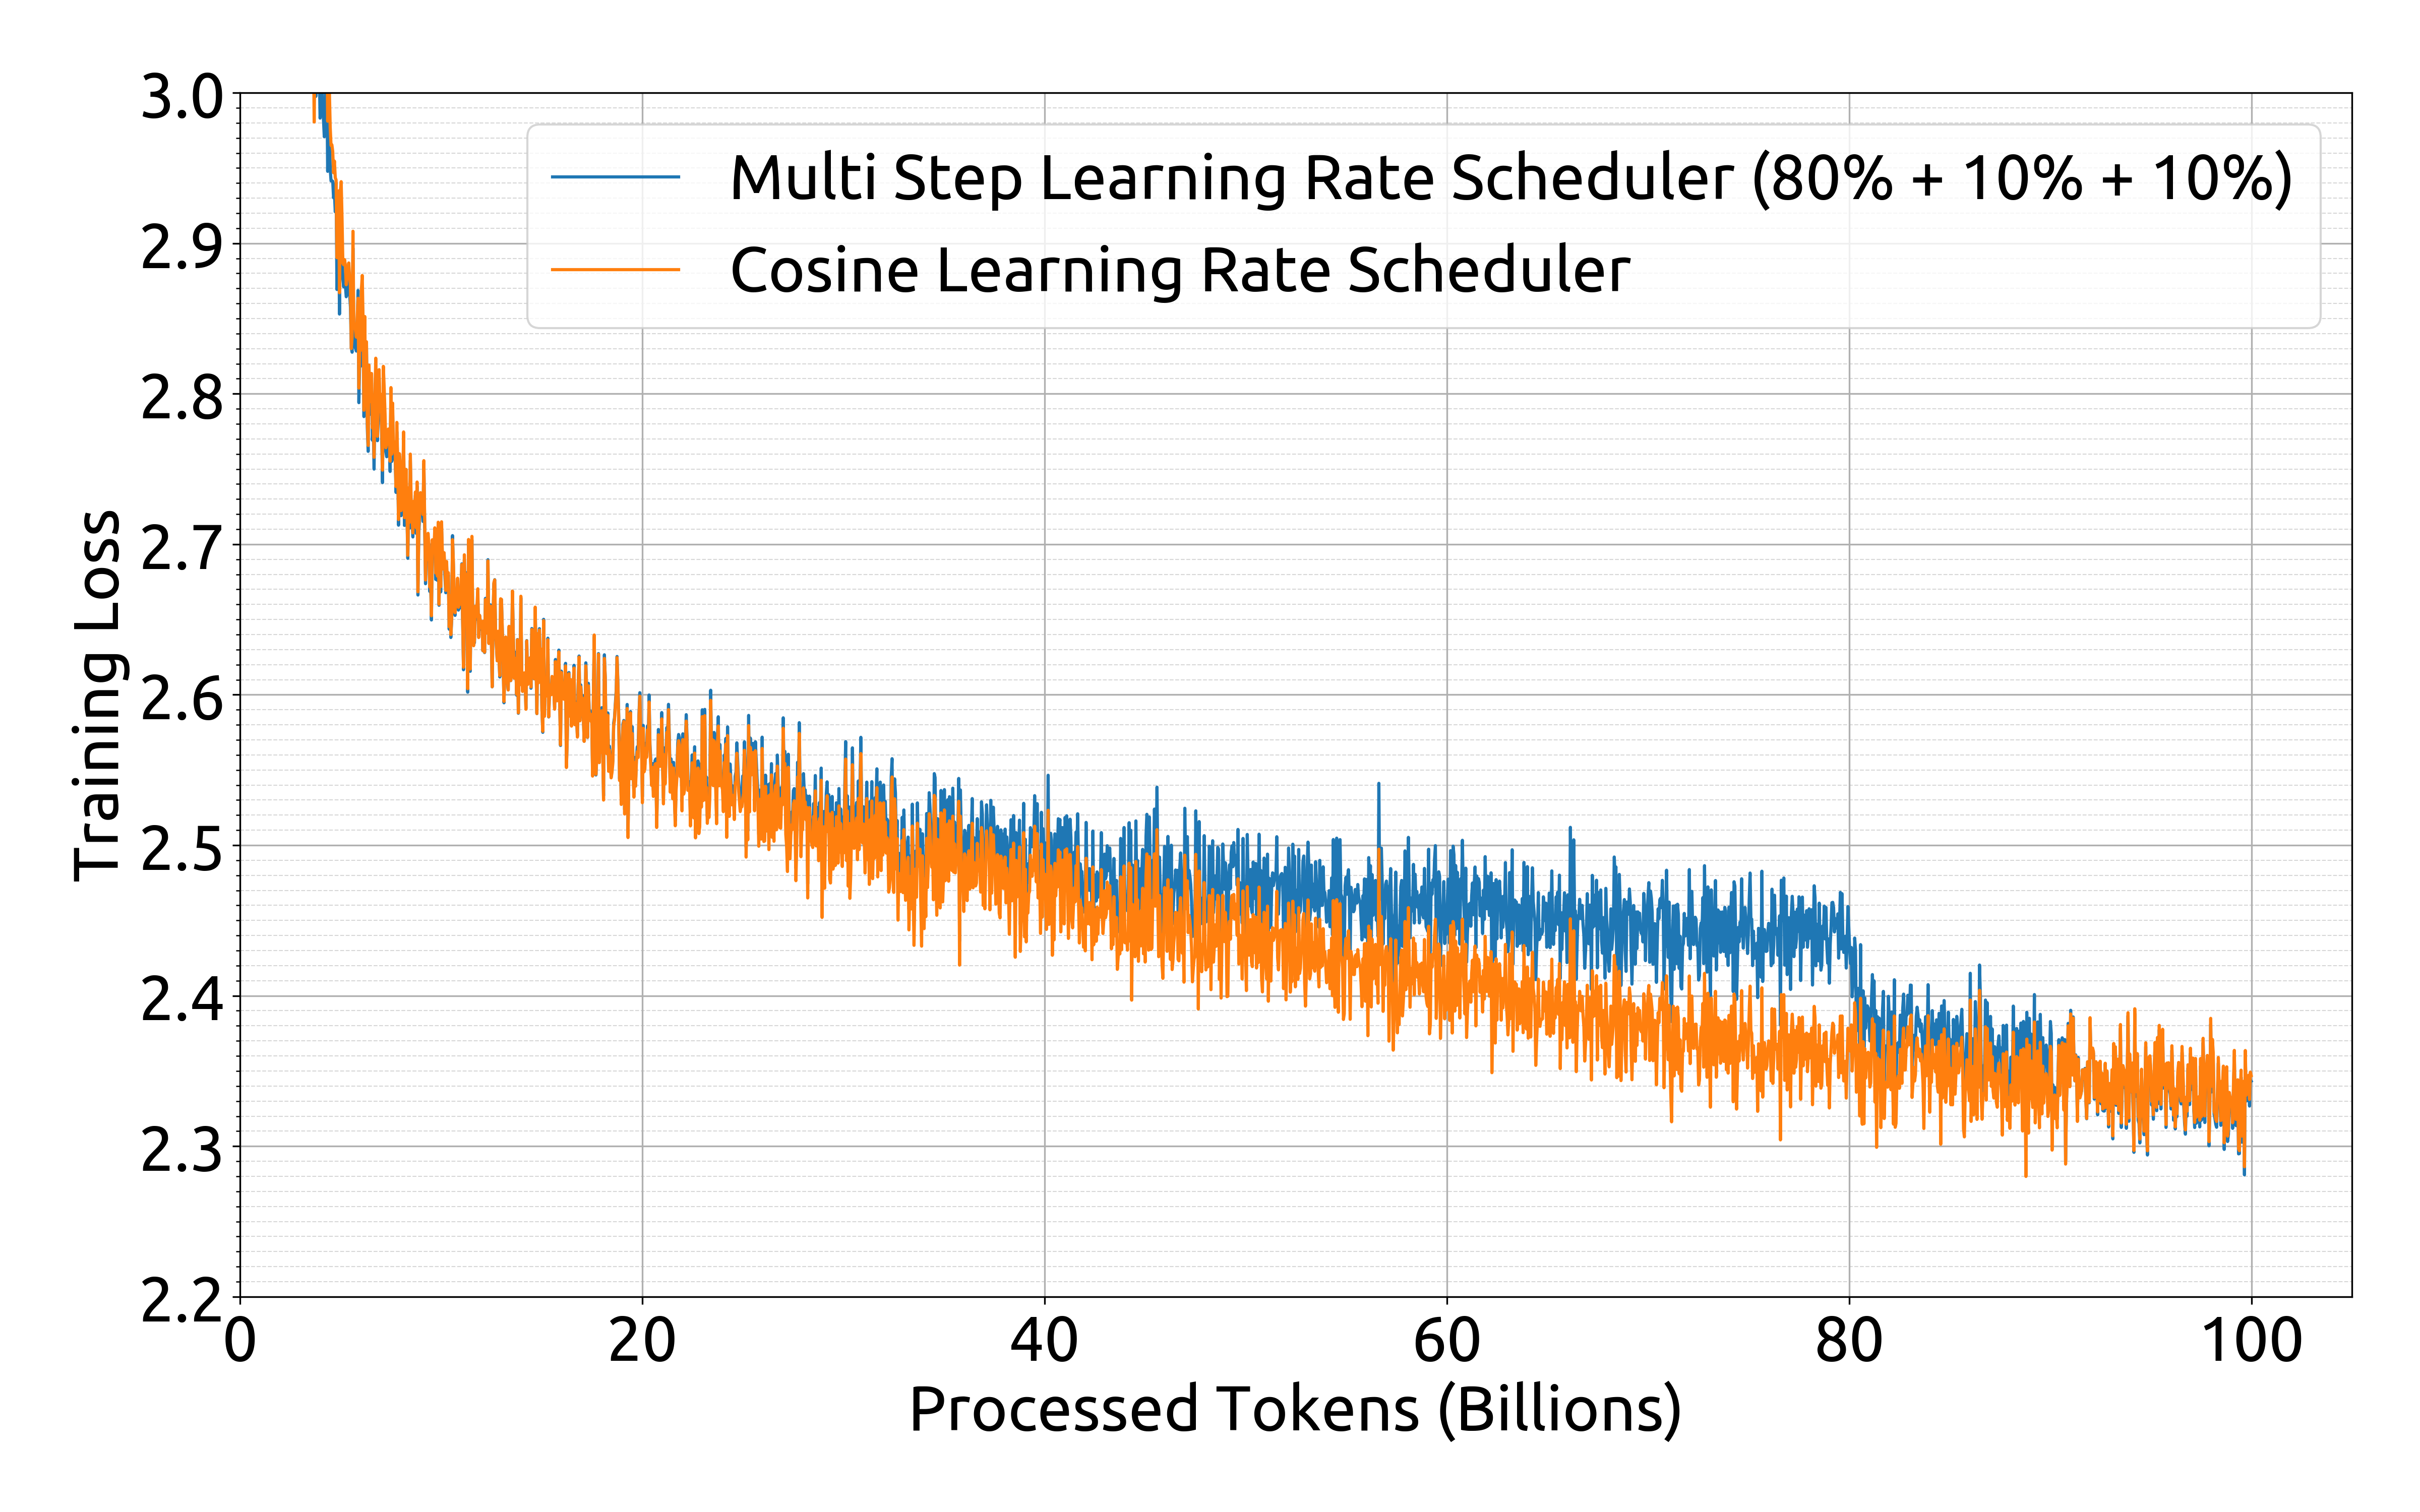
\includegraphics[width=0.48\textwidth]{figures/loss_step_cosine.png}
        \label{fig:loss_step_cosine}
    }
    \subfigure[Different proportions of multi-step stages]{
        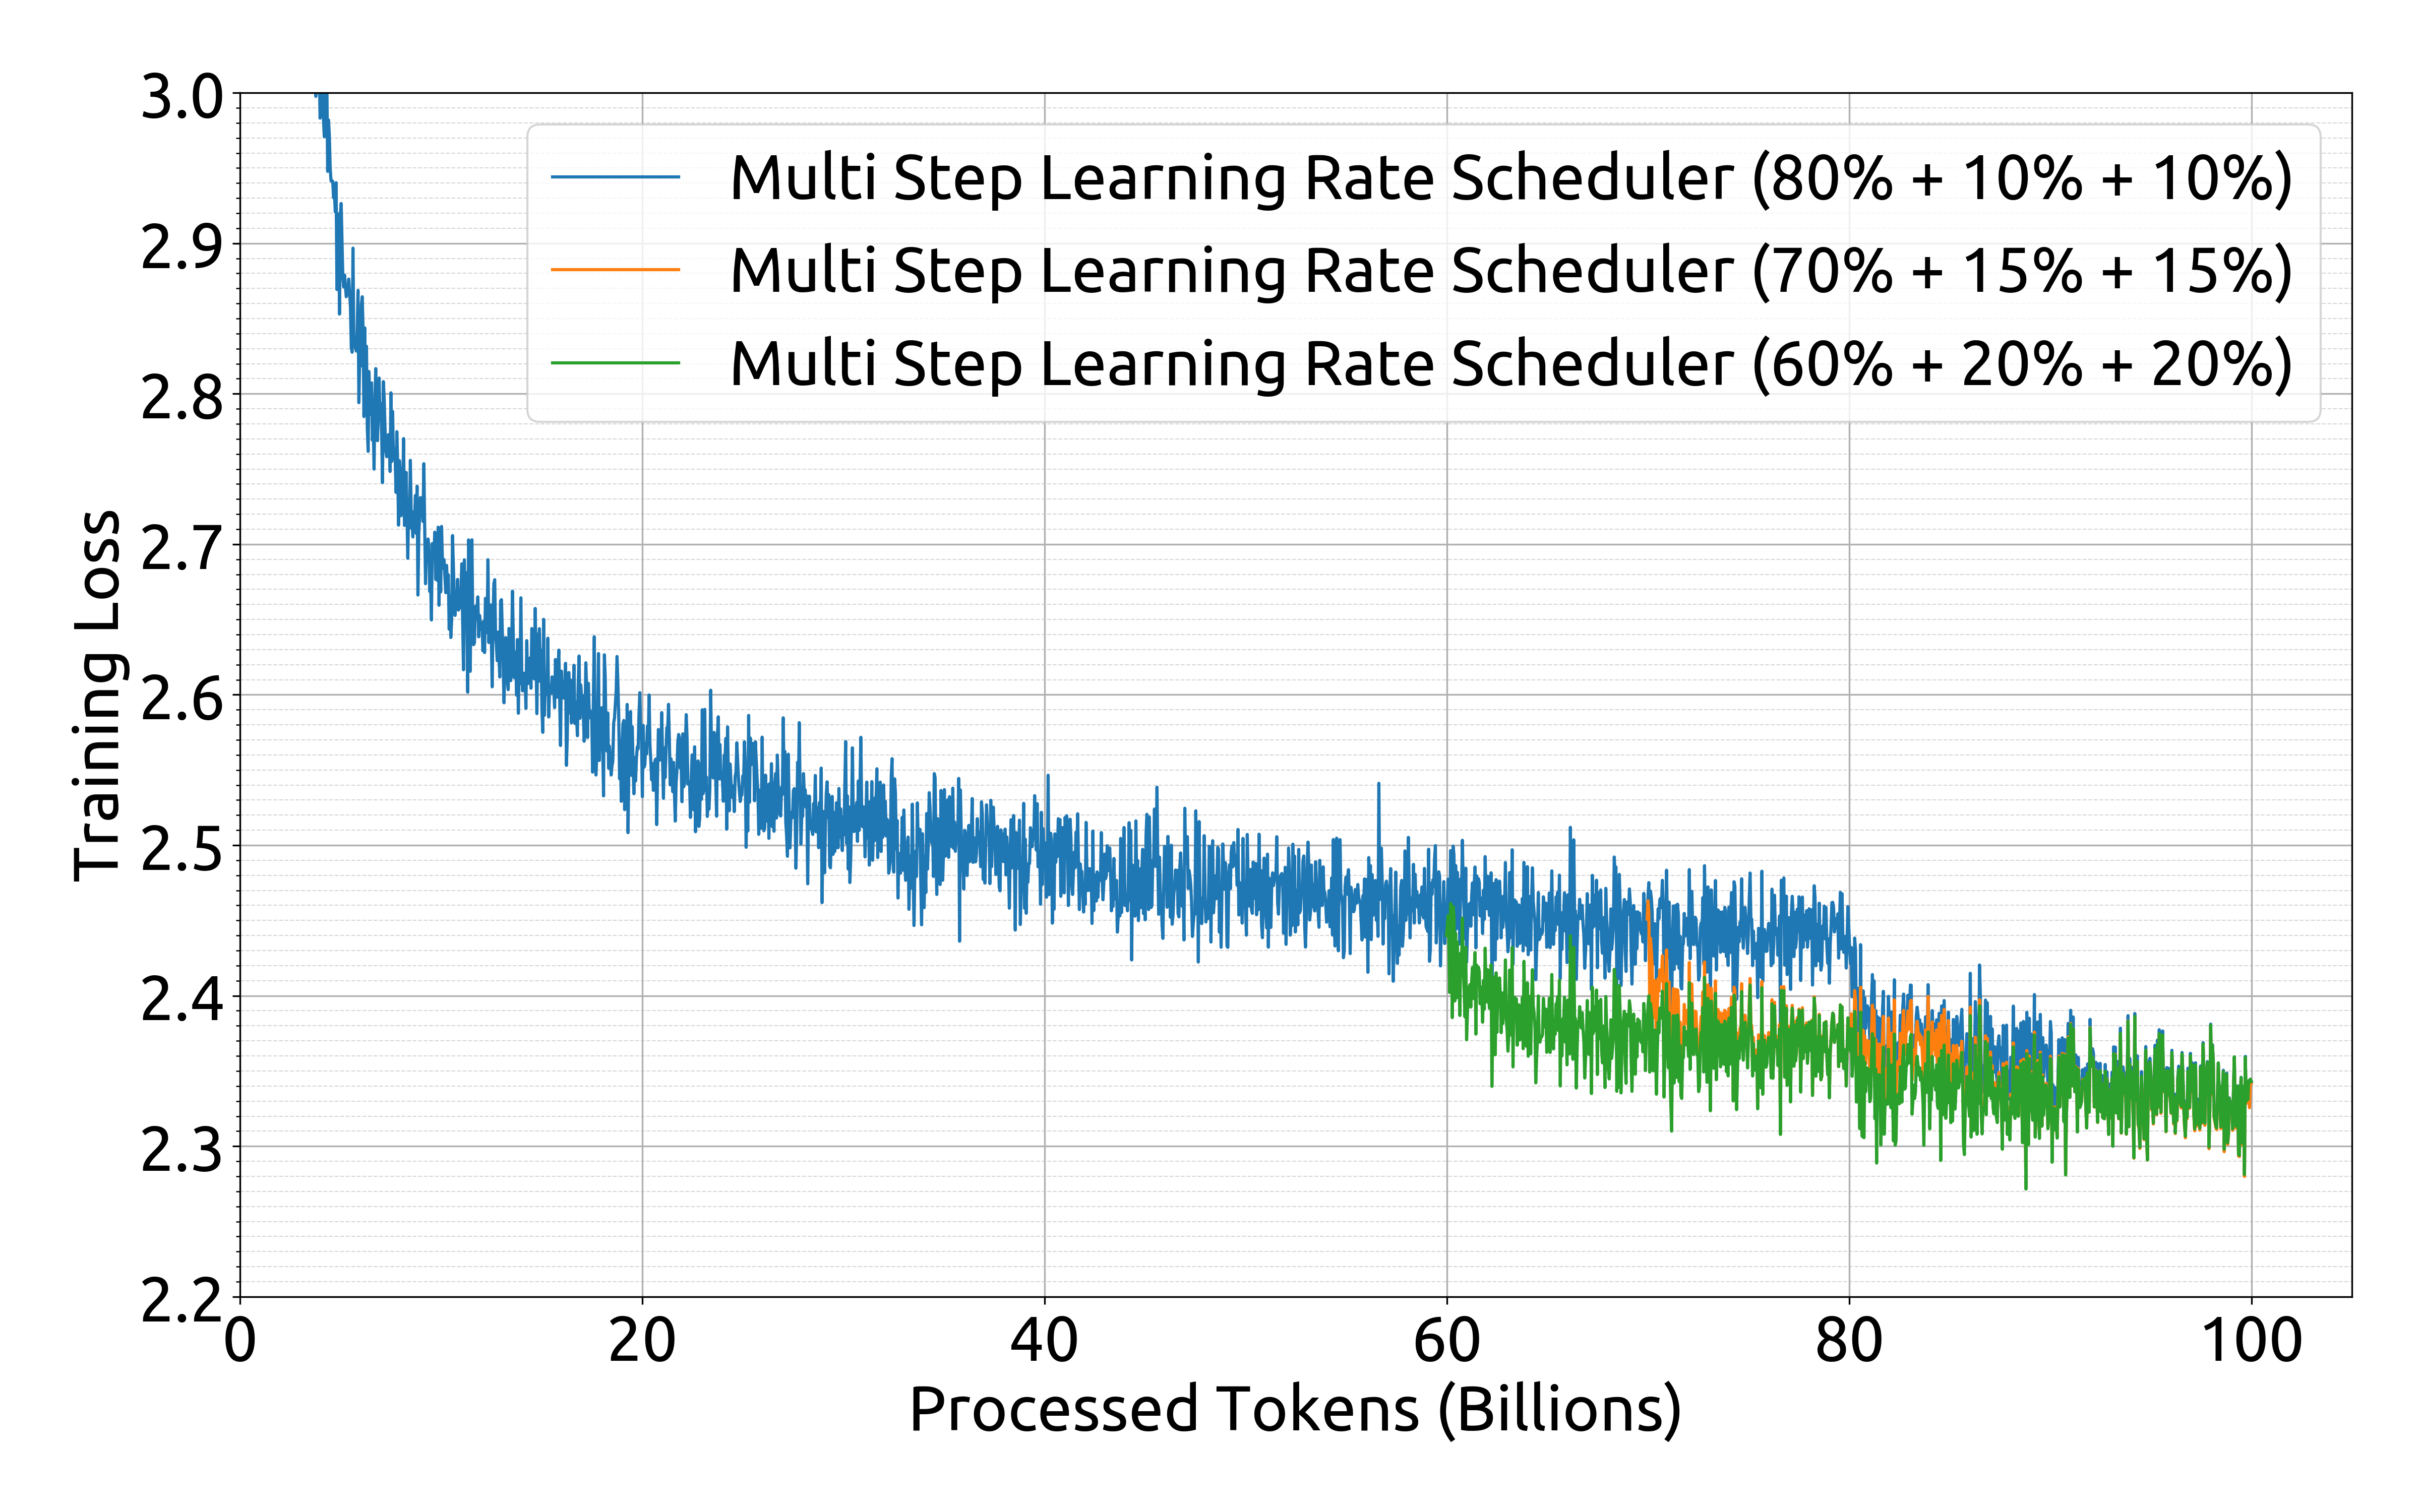
\includegraphics[width=0.48\textwidth]{figures/loss_diff_step.png}
        \label{fig:loss_diff_step}
    }
    \caption{Training loss curves with different learning rate schedulers or different parameters for schedulers. The model size is 1.6 billion parameters, trained on a dataset of 100 billion tokens.}
    \label{fig:lr_sched_opt}
\end{figure}

The batch size and learning rate vary with the model size. Specific parameters for the pre-training phases of the 7B and 67B models can be found in Table ~\ref{tab:architecture}.

\subsection{Infrastructures}
We use an efficient and light-weight training framework named HAI-LLM \citep{haillm} to train and evaluate large language models. Data parallelism, tensor parallelism, sequence parallelism, and 1F1B pipeline parallelism are integrated into this framework as done in Megatron \citep{megatron, megatron2, megatron3}. We also leverage the flash attention \citep{dao2022flashattention, dao2023flashattention2} technique to improve hardware utilization. ZeRO-1 \citep{zero} is exploited to partition optimizer states over data parallel ranks. Efforts are also made to overlap computation and communication to minimize additional waiting overhead, including the backward procedure of the last micro-batch and reduce-scatter operation in ZeRO-1, and GEMM computation and all-gather/reduce-scatter in sequence parallel. Some layers/operators are fused to speed up training, including LayerNorm, GEMM whenever possible, and Adam updates. To improve model training stability, we train the model in bf16 precision but accumulate gradients in fp32 precision. In-place cross-entropy is performed to reduce GPU memory consumption, i.e.: we convert bf16 logits to fp32 precision on the fly in the cross-entropy CUDA kernel (instead of converting it beforehand in HBM), calculate the corresponding bf16 gradient, and overwrite logits with its gradient.

Model weights and optimizer states are saved every 5 minutes asynchronously, which means we will lose no more than 5 minutes of training in the worst case of occasional hardware or network failures. These temporary model checkpoints are cleared up regularly to avoid consuming too much storage space. We also support resuming training from a different 3D parallel configuration to cope with dynamic changes in computing cluster load.

As for evaluation, we employ vLLM \citep{vllm} in generative tasks, and continuous batching in non-generative tasks to avoid manual batch size tuning and reduce token padding.

\section{Scaling Laws}
\label{sec:scaling}
Research on scaling laws~\citep{hestness2017deep} predates the emergence of large language models. Scaling laws~\citep{scalinglaw,henighan2020scaling,chinchilla} suggest that model performance can be predictably improved with increases in compute budget $C$, model scale $N$, and data scale $D$. 
When model scale $N$ is represented by model parameters and data scale $D$ by the number of tokens, $C$ can be approximated as $C=6ND$. Therefore, how to optimize the allocation between model and data scales when increasing the compute budget is also a crucial research objective in scaling laws.

The development of LLMs~\citep{dai2019transformer,gpt2}, with larger models achieving unexpected and significant performance improvements, has brought scaling laws research to a new peak. Results in scaling laws demonstrate that expanding the compute budget continues to yield significant benefits, which further encourages the increase in model scales~\citep{brown2020language,smith2022using}.

However, as shown in Table~\ref{tab:scaling_allocate_coeff}, early works~\citep{scalinglaw,chinchilla} on the optimal model/data scaling-up allocation strategy have shown varying conclusions, raising doubts about the general applicability of scaling laws. Moreover, these studies often lacked a complete description of hyperparameter settings, leaving it uncertain whether models under different compute budgets reached optimal performance. Therefore, we revisit scaling laws in this section to address these uncertainties and ensure we are on the right path to efficiently scale-up compute, which reflects the long-term perspective and is key to developing continuously improving models.

To ensure that models under different compute budgets can achieve optimal performance, we first studied the scaling laws of hyperparameters. Empirically, it has been observed that the optimal values of most parameters during training do not change when varying compute budgets. Therefore, these parameters are consistent with those outlined in Section~\ref{sec:intro-hyper-params} and remain unchanged across different compute budgets. However, the hyperparameters that have the most significant impact on performance, namely batch size and learning rate, were re-examined.

Early works~\citep{mccandlish2018empirical,shallue2019measuring,smith2017don,goyal2017accurate, zhang2019algorithmic} provided some empirical observations for setting batch size and learning rate, but we found these observations have limited applicability in our preliminary experiments.
Through extensive experiments, we modeled the power law relationship between the compute budget $C$ and the optimal batch size and learning rate. This relationship, which we refer to as the scaling laws of hyperparameters, provides an empirical framework for determining the optimal hyperparameters. This methodology ensures that models across different compute budgets can reach their near-optimal performance.

We then study the scaling laws of the model and data scales. To reduce experimental costs and fitting difficulties, we adopted the IsoFLOP profile approach from Chinchilla~\citep{chinchilla} to fit the scaling curve. To represent the model scale more accurately, we utilized a new model scale representation, non-embedding FLOPs/token $M$, replacing the earlier-used model parameters $N$, and substituted the approximate compute budget formula $C=6ND$ with the more precise $C=MD$.
The experimental results provided insights into the optimal model/data scaling-up allocation strategy and performance predictions, and also accurately forecasted the expected performance of DeepSeek LLM 7B and 67B models.

Additionally, in the process of exploring scaling laws, the data we used underwent multiple iterations, continually improving in quality. We attempted to fit the scaling curve on various datasets and found that the data quality significantly influences the optimal model/data scaling-up allocation strategy. The higher the data quality, the more the increased compute budget should be allocated to model scaling. 
This implies that high-quality data can drive the training of larger models given the same data scale. The differences in the optimal model/data scaling-up allocation strategy may also serve as an indirect approach to assess the quality of data. We will continue to pay close attention to the changes in data quality and its impact on scaling laws, and provide more analysis in future works. 


In summary, our contributions and findings in scaling laws can be summarized as follows:
\begin{itemize}
    \item We established the scaling laws for hyperparameters, providing an empirical framework for determining the optimal hyperparameters.
    \item Instead of model parameters $N$, we adopt non-embedding FLOPs/token $M$ to represent the model scale, leading to a more accurate optimal model/data scaling-up allocation strategy and a better prediction of generalization loss for large-scale models.
    \item The quality of pre-training data impacts the optimal model/data scaling-up allocation strategy. The higher the data quality, the more the increased compute budget should be allocated to model scaling.
\end{itemize}

\subsection{Scaling Laws for Hyperparameters}
We initially conducted a grid search for batch size and learning rate on small-scale experiments with a compute budget of 1e17, and the results of a specific model size (177M FLOPs/token) are illustrated in Figure~\ref{fig:loss_bs_lr_1e17}. The results demonstrate that the generalization error remains stable across a wide range of choices of batch sizes and learning rates. This indicates that near-optimal performance can be achieved within a relatively wide parameter space.

\begin{figure}[h]
    \centering
    \subfigure[1e17 FLOPs (177M FLOPs/token)]{
        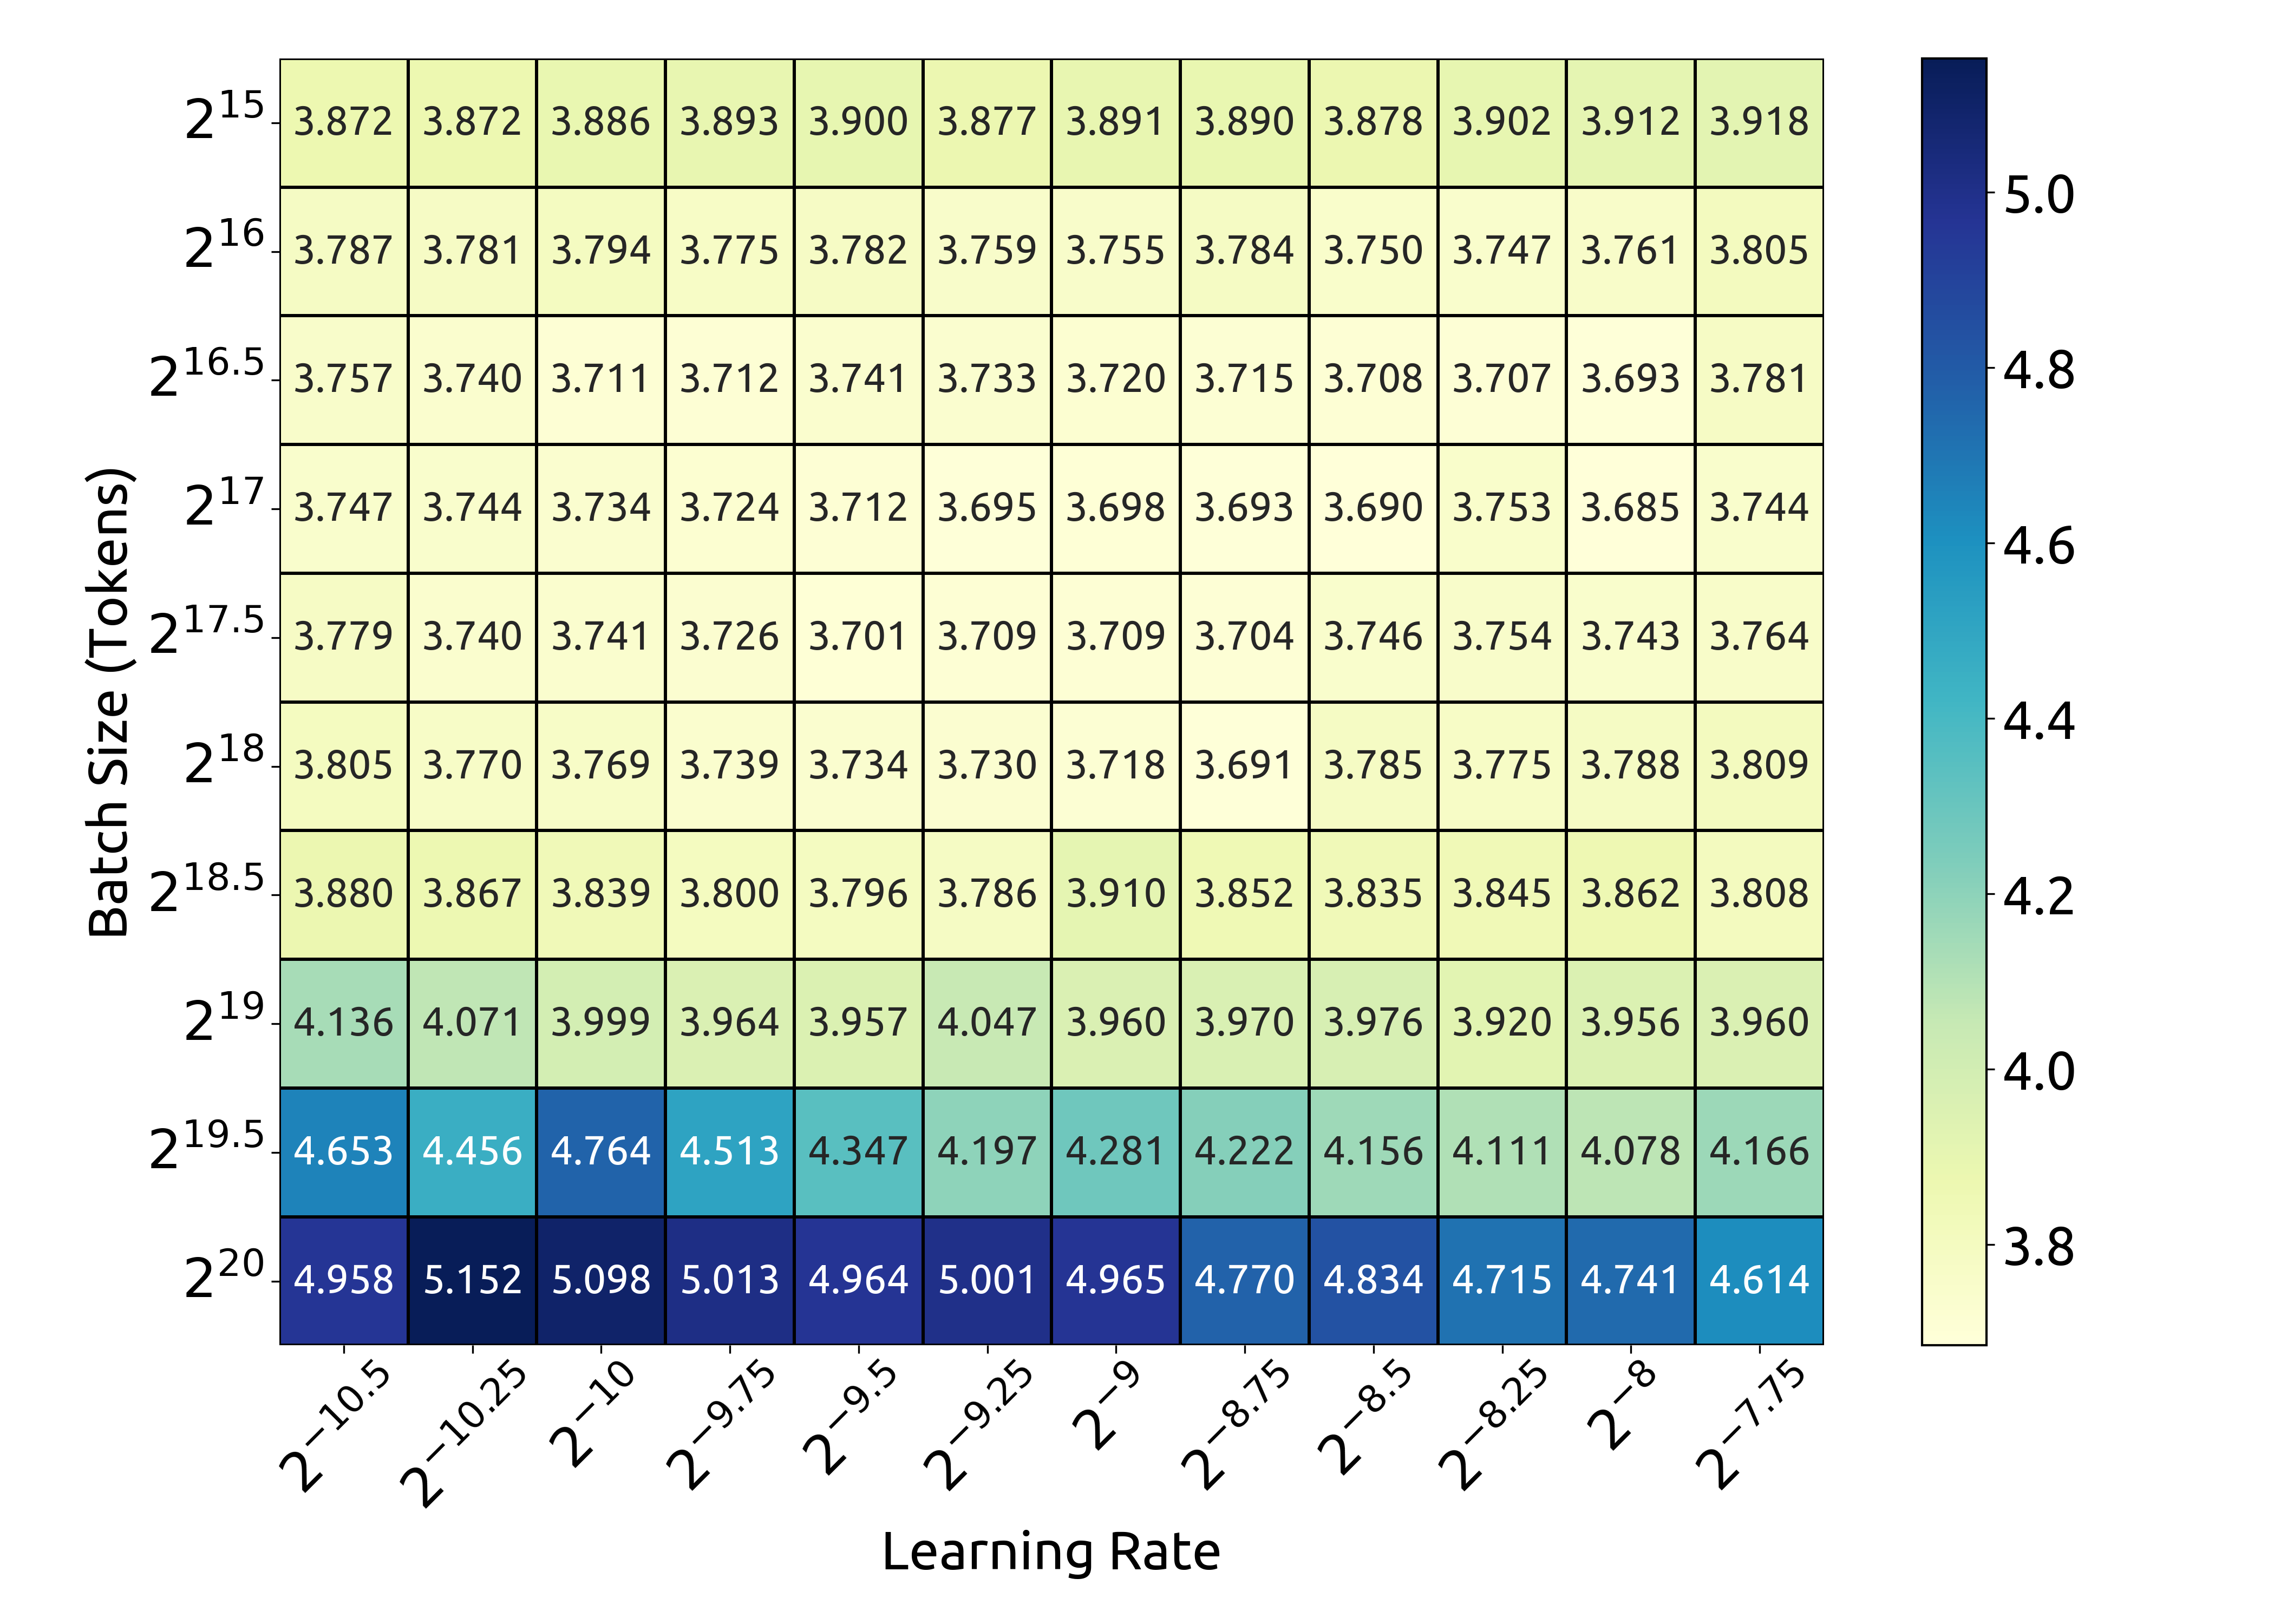
\includegraphics[width=0.48\textwidth]{figures/loss_bs_lr_1e17.png}
        \label{fig:loss_bs_lr_1e17}
    }
    \subfigure[1e20 FLOPs (2.94B FLOPs/token)]{
        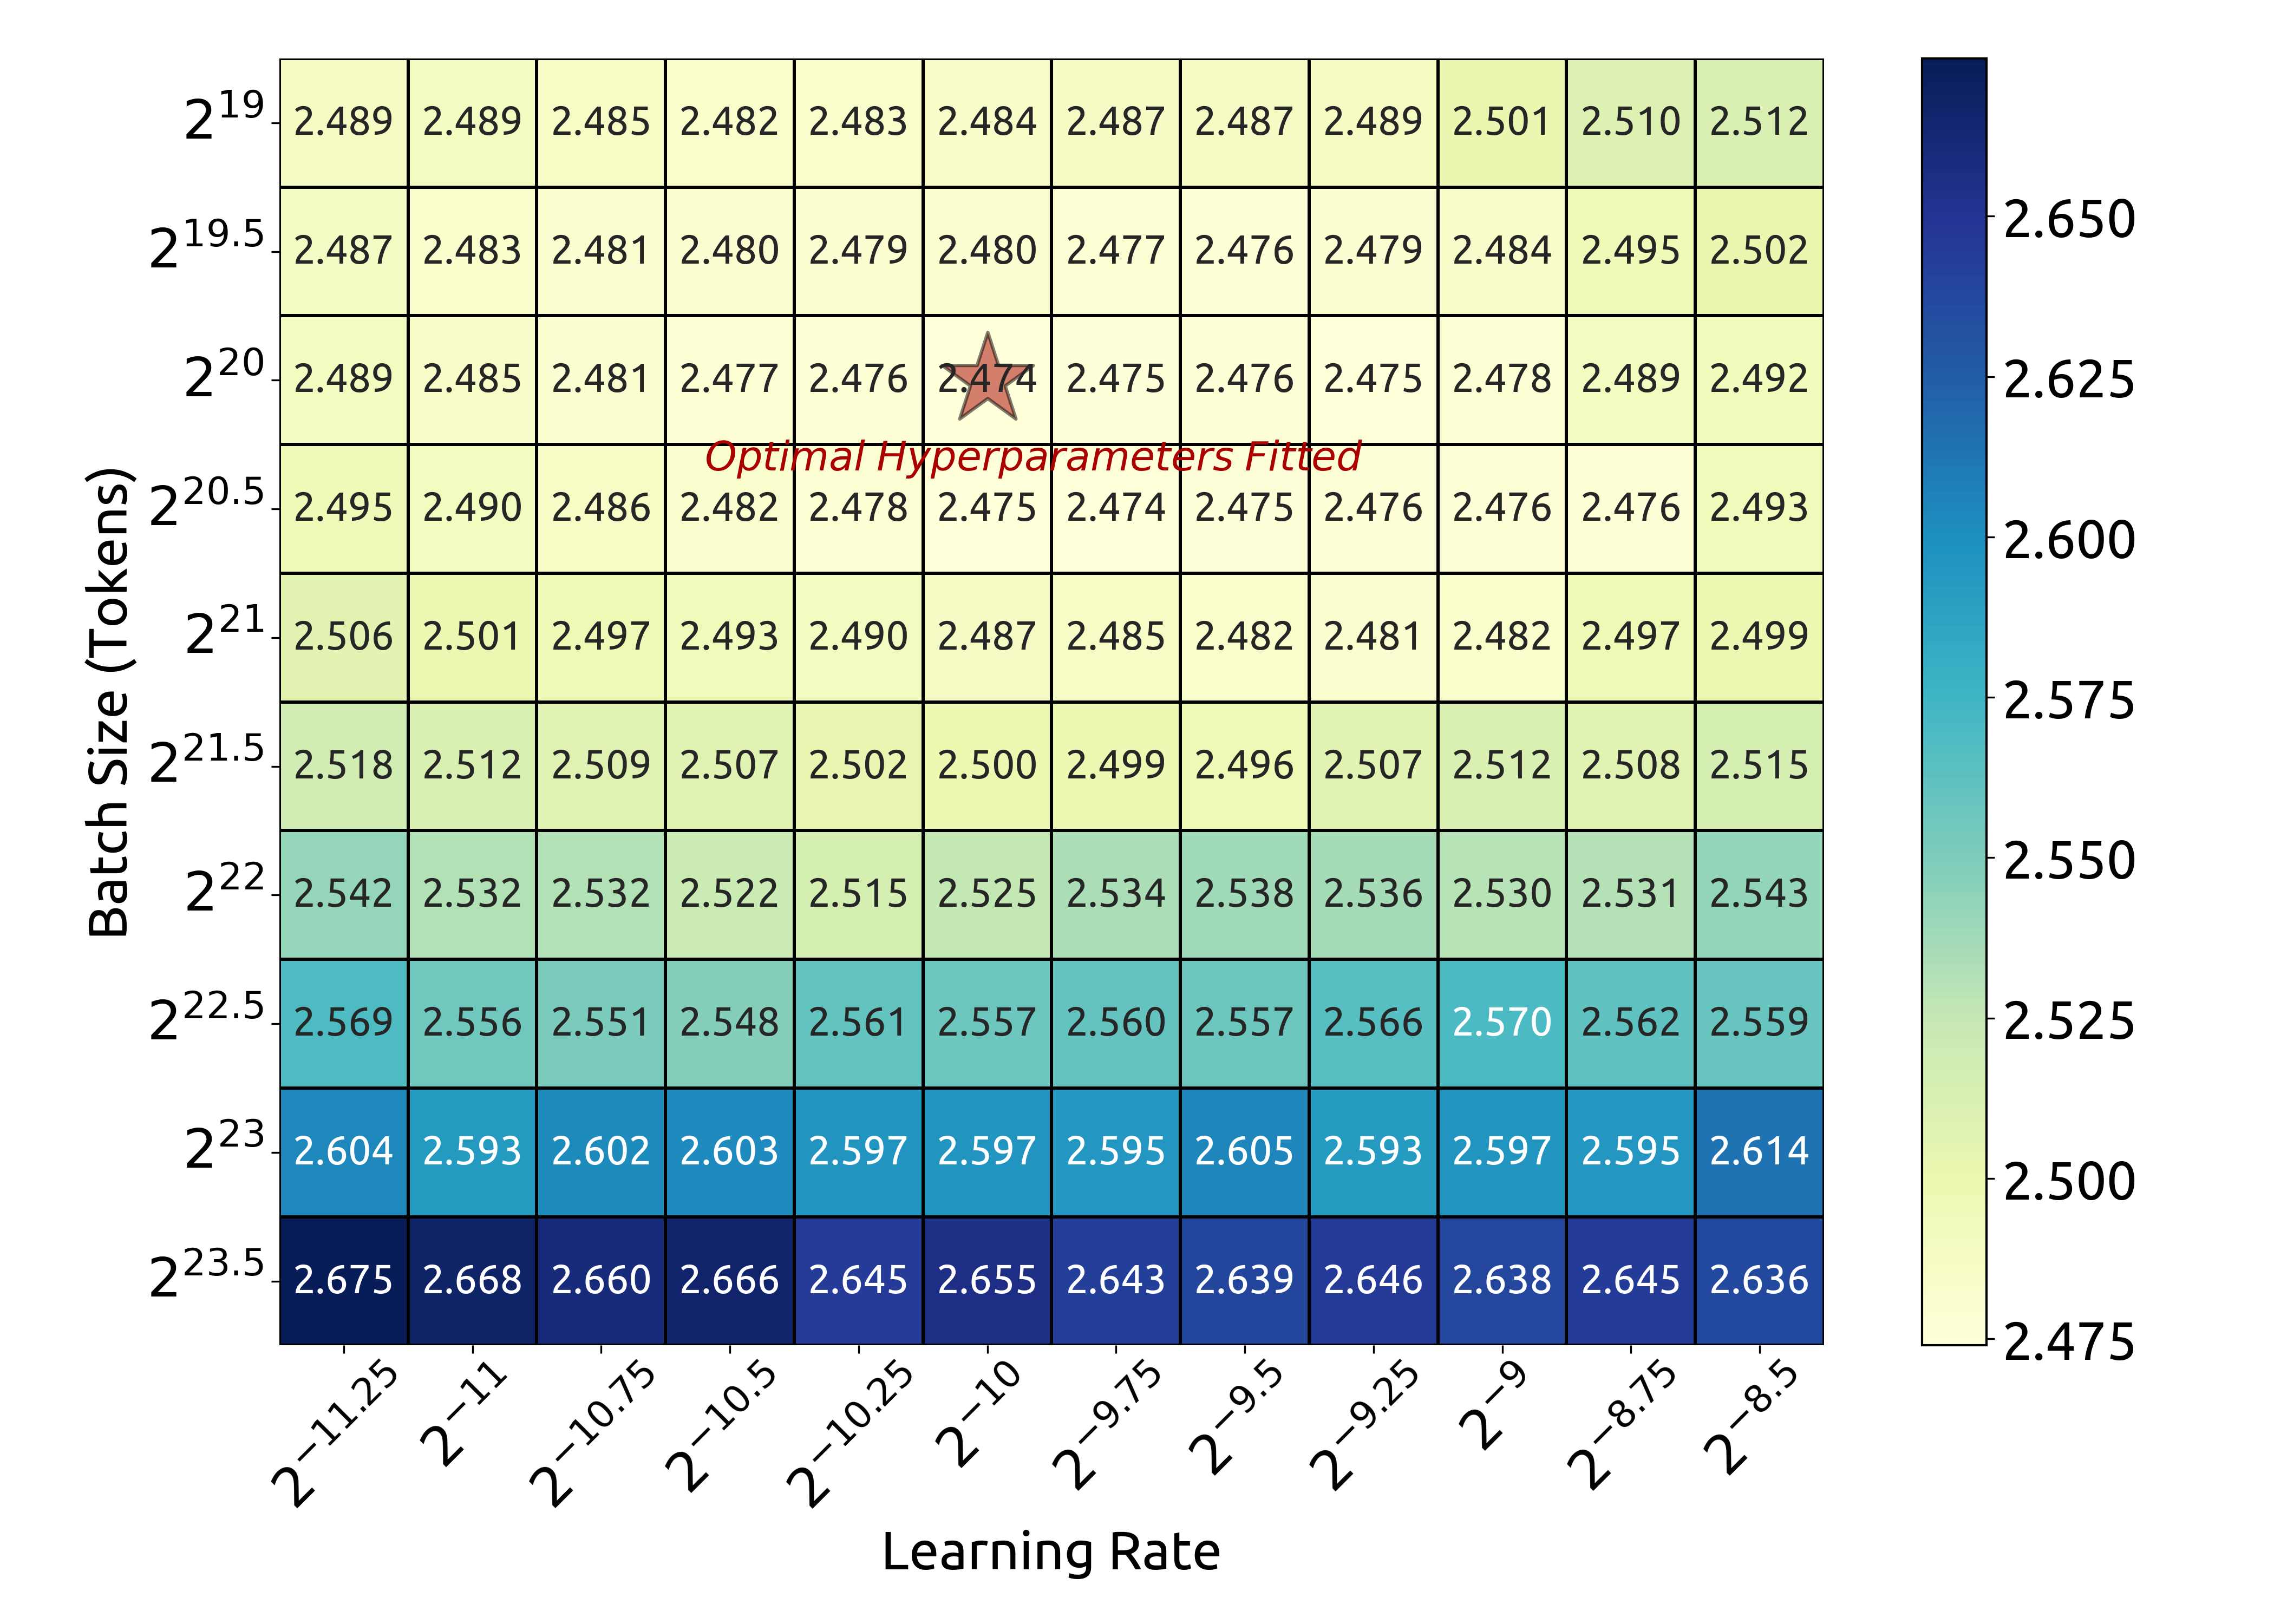
\includegraphics[width=0.48\textwidth]{figures/loss_bs_lr_1e20.png}
        \label{fig:loss_bs_lr_1e20}
    }
    \caption{\centering Training loss w.r.t. batch size and learning rate with 1e17 and 1e20 FLOPs.}
    \label{fig:loss_bs_lr_1e17_1e20}
\end{figure}

Then, we utilized the aforementioned multi-step learning rate scheduler to effectively train multiple models with different batch sizes, learning rates, and compute budgets ranging from 1e17 to 2e19 by reusing the first stage. Considering the redundancy in the parameter space, we regarded the parameters used by models whose generalization error exceeded the minimum by no more than 0.25\% as near-optimal hyperparameters. We then fitted the batch size $B$ and learning rate $\eta$ with respect to the compute budget $C$. The fitting results, as shown in Figure~\ref{fig:flops_bsz_lr_fitting}, reveal that the optimal batch size $B$ gradually increases with the increase in compute budget $C$, while the optimal learning rate $\eta$ gradually decreases. This is in line with the intuitive empirical settings for batch size and learning rate when scaling up models. Moreover, all near-optimal hyperparameters fall within a broad band range, indicating that it is relatively easy to choose near-optimal parameters within this interval. The final formulae we fitted for batch size and learning rate are as follows:
\begin{equation}
\label{eqa:bsz_lr_formulae}
\begin{aligned}
    \eta_{\mathrm{opt}} &= 0.3118\cdot C^{\,-0.1250} \\
    B_{\mathrm{opt}} &= 0.2920\cdot C^{\,0.3271} 
\end{aligned}
\end{equation}

\begin{figure}[h]
    \centering
    \subfigure[Batch size scaling curve]{
        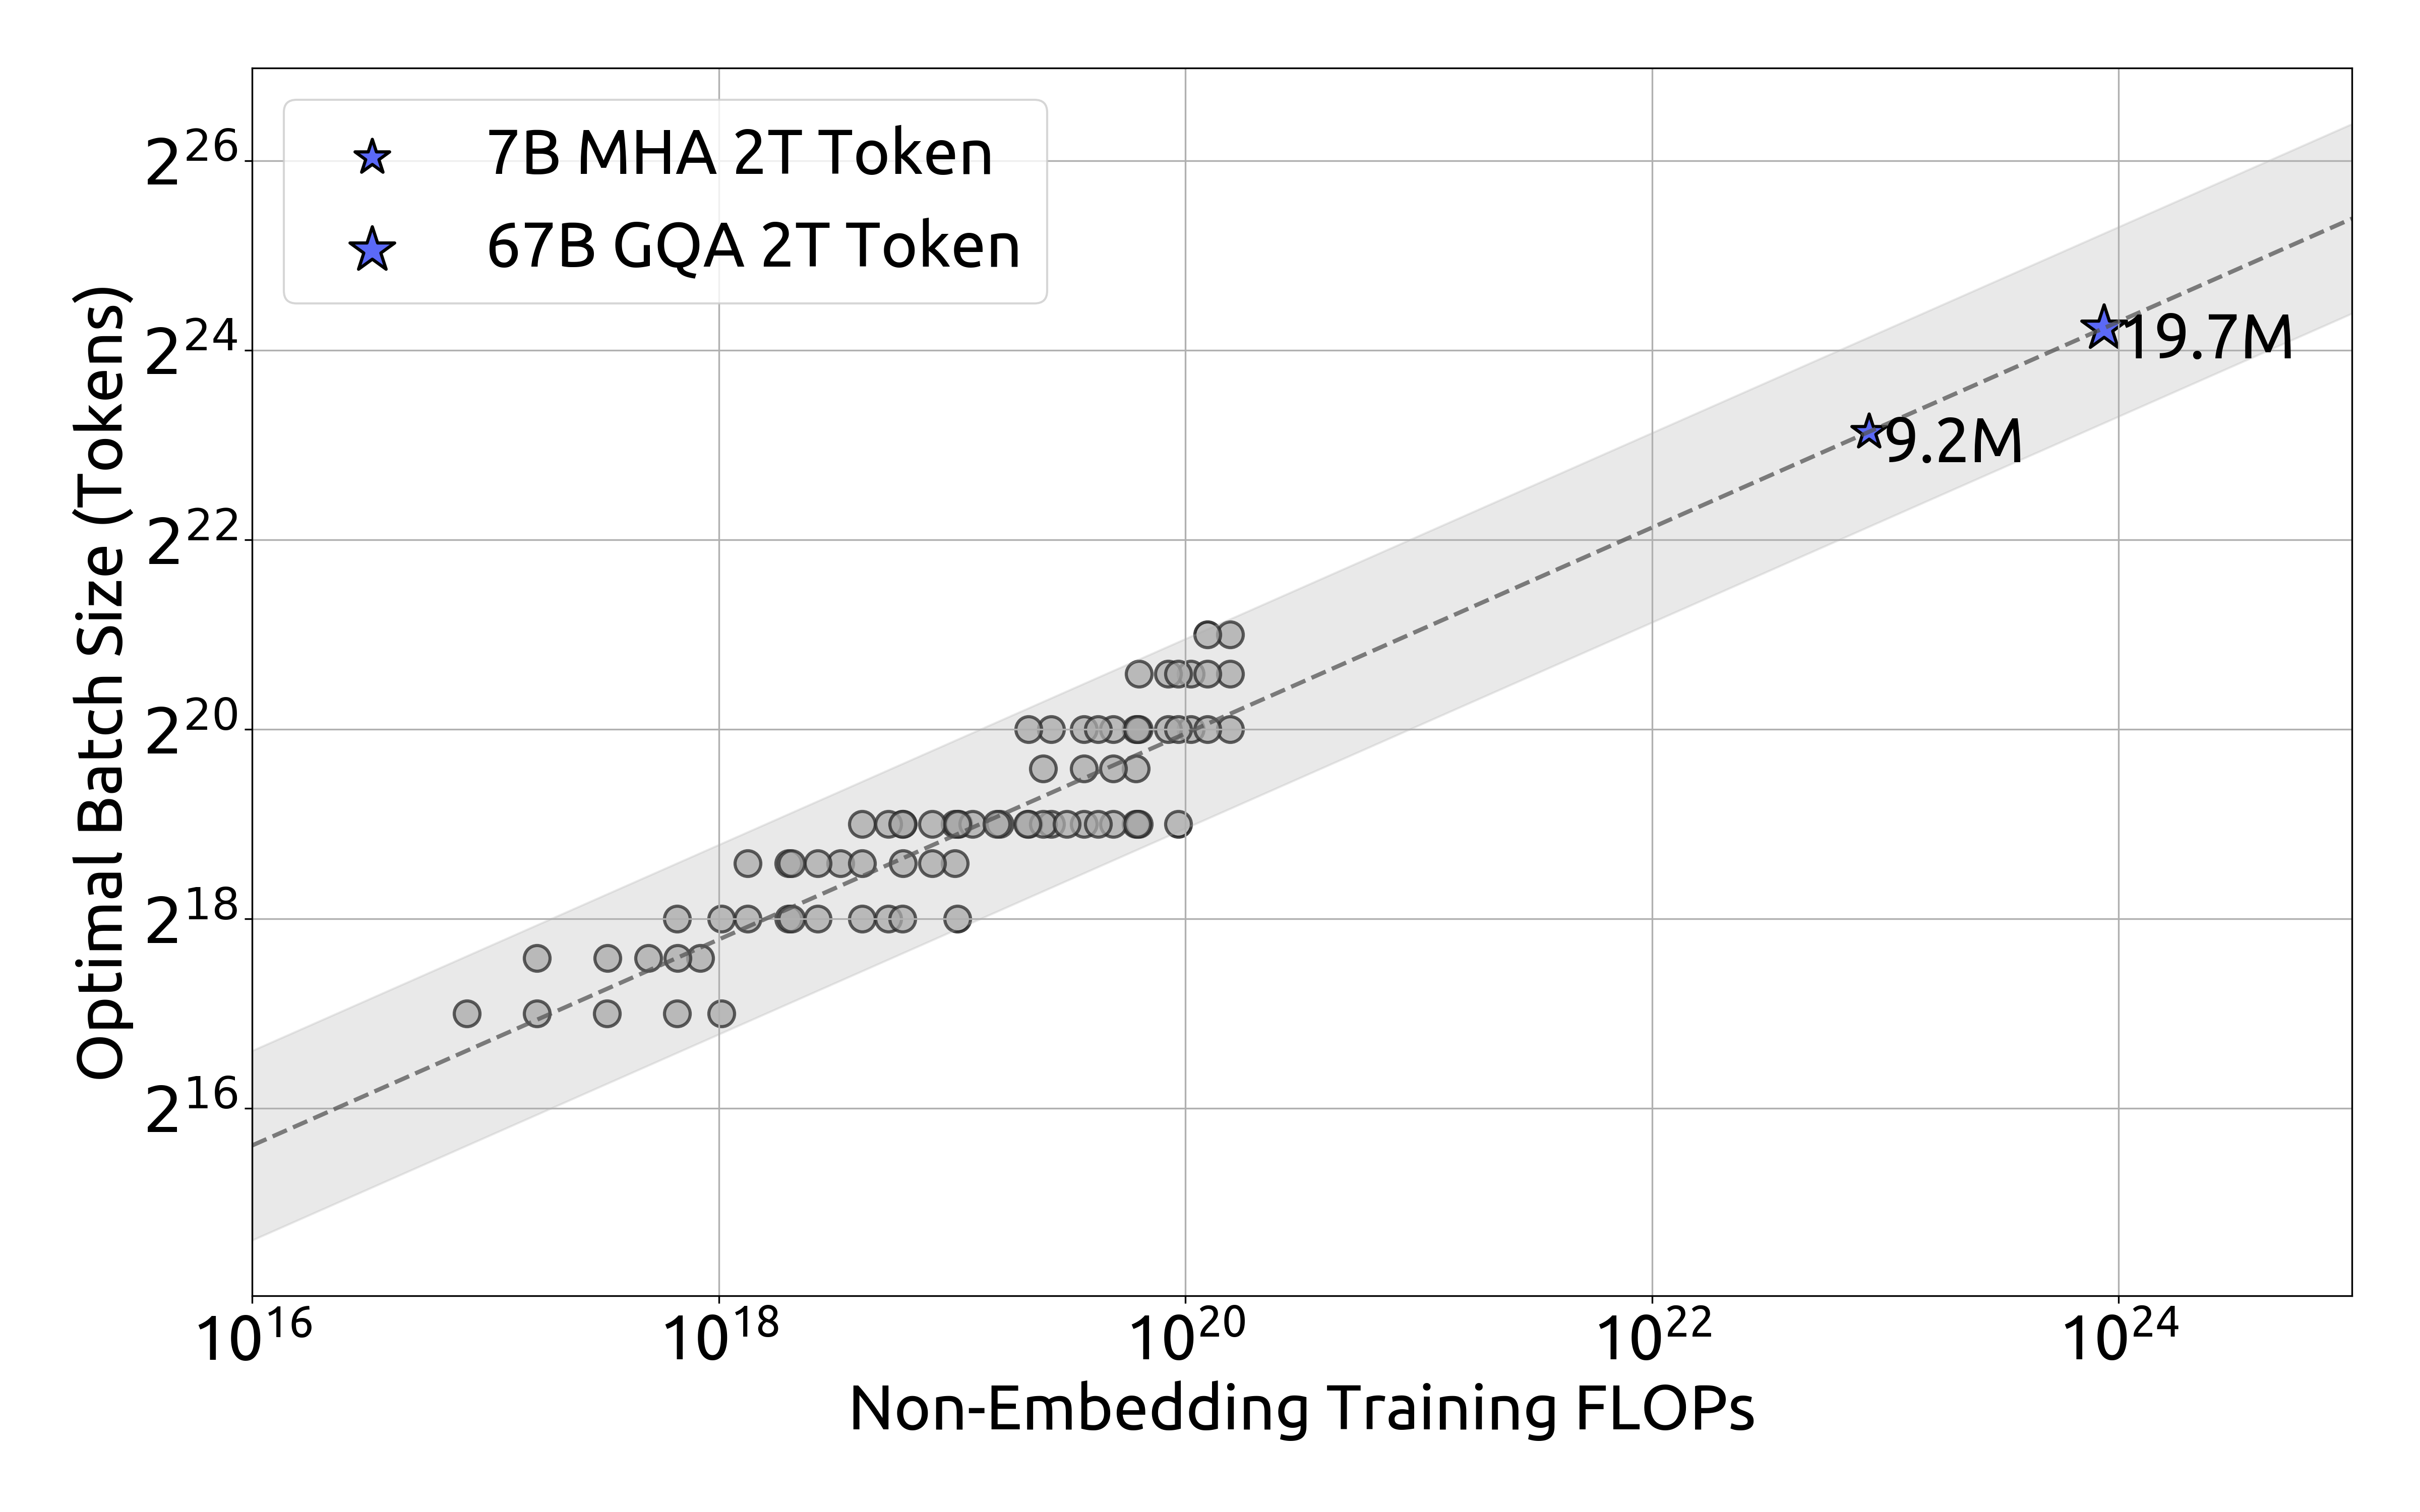
\includegraphics[width=0.48\textwidth]{figures/flops_bsz_fitting.png}
        \label{fig:flops_bsz_fitting}
    }
    \subfigure[Learning rate scaling curve]{
        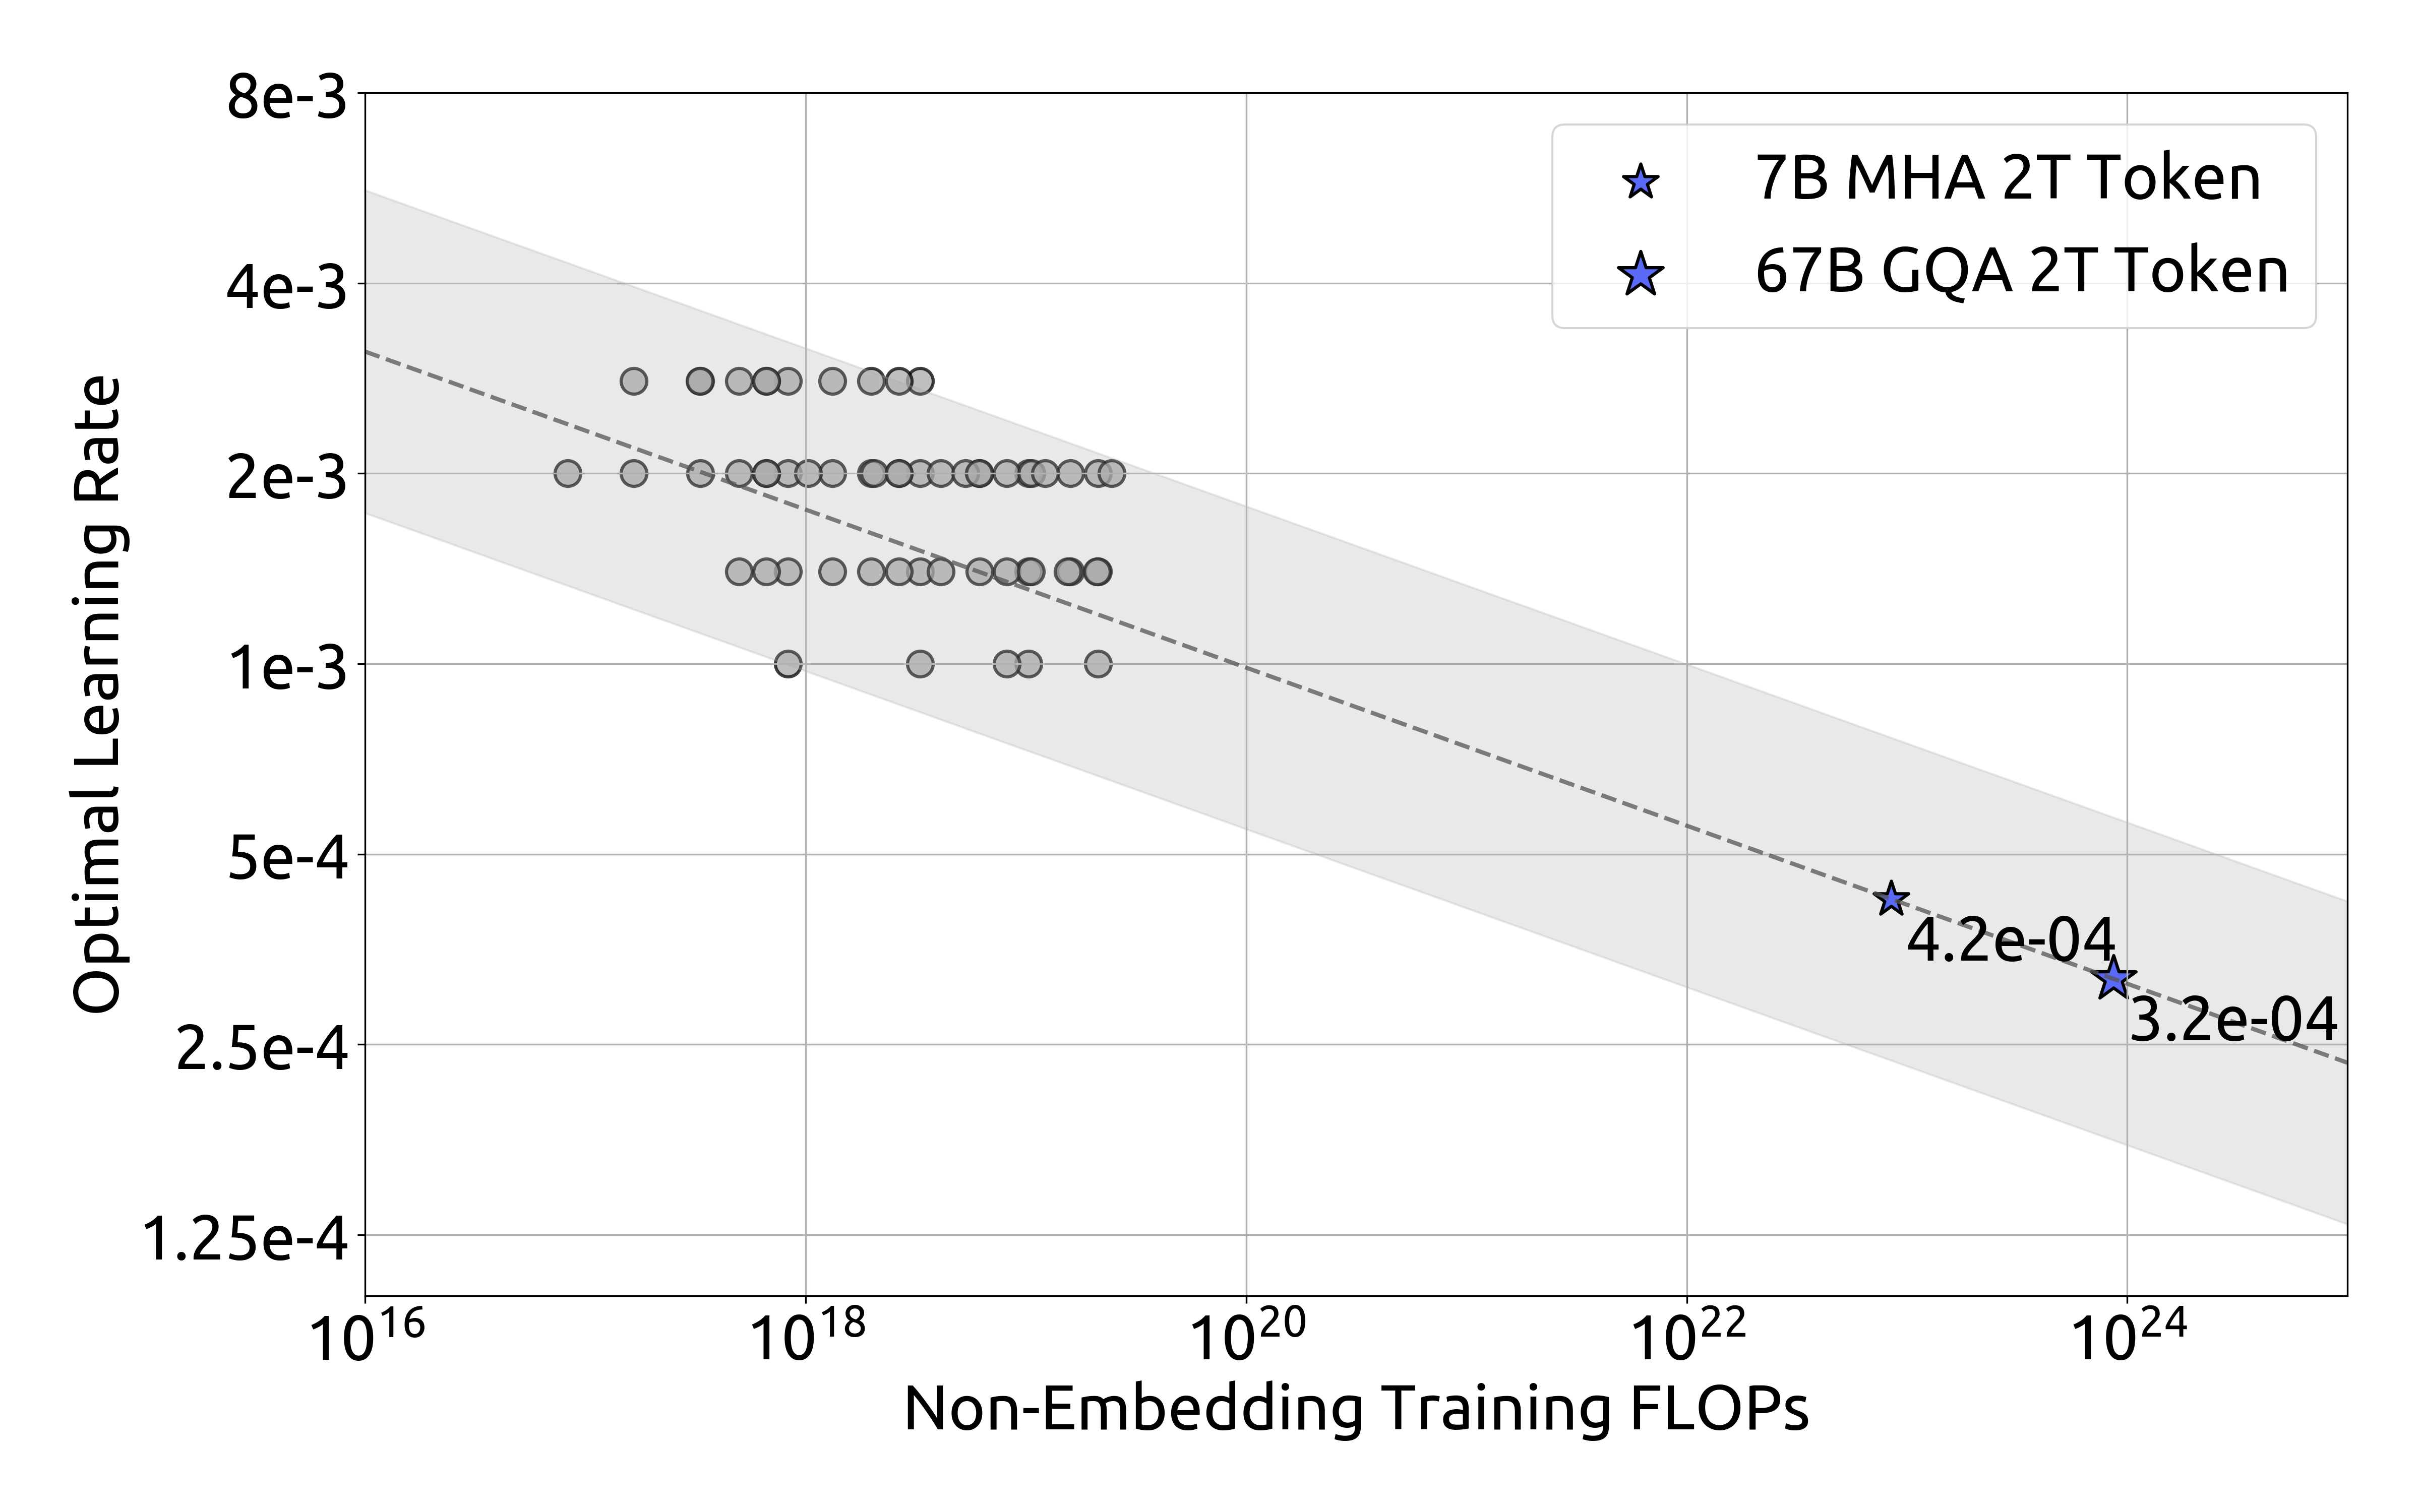
\includegraphics[width=0.48\textwidth]{figures/flops_lr_fitting.png}
        \label{fig:flops_lr_fitting}
    }
    \caption{Scaling curves of batch size and learning rate. The grey circles represent models whose generalization error exceeded the minimum by no more than 0.25\%. The dotted line represents the power law fitting the smaller model. The blue stars represent DeepSeek LLM 7B and 67B.}
    \label{fig:flops_bsz_lr_fitting}
\end{figure}


We validated our formulae on a series of models with a 1e20 compute budget, and the results of a specific model size (2.94B FLOPs per token) are shown in Figure~\ref{fig:loss_bs_lr_1e20}. The results indicate that the fitted parameters are centered in the optimal parameter space. Subsequent sections also show that the parameters we fitted for DeepSeek LLM 7B and 67B models similarly achieved good performance. 

However, it's important to note that we have not yet considered the impact of factors beyond the compute budget $C$ on the optimal hyperparameters. This is inconsistent with some earlier works~\citep{mccandlish2018empirical, scalinglaw} which suggested that the optimal batch size can be modeled as being solely related to the generalization error $L$.
Furthermore, we observed that in models with the same compute budget but different model/data allocations, the optimal parameter space varies slightly. This suggests that further research is needed to understand the selection of hyperparameters and training dynamics. We will explore these aspects in future works.

\subsection{Estimating Optimal Model and Data Scaling}

After deriving the formulae for fitting near-optimal hyperparameters, we started fitting the scaling curve and analyzing the optimal model/data scaling-up allocation strategy. 
This strategy involves finding model scaling exponent $a$ and data scaling exponent $b$ that satisfy $N_{\mathrm{opt}} \propto C^a$ and $D_{\mathrm{opt}} \propto C^b$, respectively. The data scale $D$ can be consistently represented by the number of tokens in the dataset. In previous works, the model scale was typically represented by model parameters, with non-embedding parameters $N_1$~\citep{scalinglaw} and complete parameters $N_2$~\citep{chinchilla}. The relationship between compute budget $C$ and model/data scale could be approximately described as $C=6ND$, meaning we could use $6N_1$ or $6N_2$ to approximate the model scale. However, since both $6N_1$ and $6N_2$ do not account for the computational overhead of attention operation, and $6N_2$ also includes the vocabulary computation, which contributes less to the model's capacity, they both have significant approximation errors under certain settings.

To mitigate these errors, we introduced a new model scale representation: non-embedding FLOPs/token $M$. $M$ includes the computational overhead of attention operation but does not take into account the vocabulary computation. With the model scale represented by $M$, the compute budget $C$ can be simply expressed as $C=MD$. The specific differences between $6N_1$, $6N_2$, and $M$ are as shown in the following formulae:
\begin{equation}
\label{eqa:diff_model_scale}
\begin{aligned}
    6N_1 &= 72\,n_{\mathrm{layer}}\,d_{\mathrm{model}}^2 \\
    6N_2 &= 72\,n_{\mathrm{layer}}\,d_{\mathrm{model}}^2 + 6\,n_{\mathrm{vocab}}\,d_{\mathrm{model}} \\
    M &= 72\,n_{\mathrm{layer}}\,d_{\mathrm{model}}^2 + 12\,n_{\mathrm{layer}}\,d_{\mathrm{model}}\,l_{\mathrm{seq}}
\end{aligned}
\end{equation}
where $n_{\mathrm{layer}}$ represents the number of layers, $d_{\mathrm{model}}$ represents the model width, $n_{\mathrm{vocab}}$ is the vocabulary size, and $l_{\mathrm{seq}}$ is the sequence length. We assessed the differences between these three representations across models of varying scales, as shown in Table~\ref{tab:6nd_approximation_error}. The results indicate that both $6N_1$ and $6N_2$ either overestimate or underestimate the computational cost in models of different scales. This discrepancy is particularly pronounced in small-scale models, with differences reaching up to 50\%. Such inaccuracies can introduce substantial statistical errors when fitting the scaling curve. Please refer to Appendix~\ref{appendix:diff_model_scale_repre} for further analysis regarding different representations of model scale.


\begin{table}[h]
    \centering
    \begin{tabular}{cccc|ccc|cc}
    \toprule
        $n_{\mathrm{layers}}$ & $d_{\mathrm{model}}$ & $n_{\mathrm{vocab}}$ & $l_{\mathrm{seq}}$ & $N_{1}$ & $N_{2}$ & $M$ & $\frac{6N_1}{M}$ & $\frac{6N_2}{M}$ \\
    \midrule
        8   & 512  & \multirow{7}{*}{102400} & \multirow{7}{*}{4096} & 25.2M & 77.6M & 352M  & 0.43 & 1.32 \\
        12  & 768  &  &  & 84.9M & 164M  & 963M  & 0.53 & 1.02 \\
        24  & 1024 &  &  & 302M  & 407M  & 3.02B & 0.60 & 0.81 \\
        24  & 2048 &  &  & 1.21B & 1.42B & 9.66B & 0.75 & 0.88 \\
        32  & 4096 &  &  & 6.44B & 6.86B & 45.1B & 0.85 & 0.91 \\
        40  & 5120 &  &  & 12.6B & 13.1B & 85.6B & 0.88 & 0.92 \\
        80  & 8192 &  &  & 64.4B & 65.3B & 419B  & 0.92 & 0.94 \\
    \bottomrule
    \end{tabular}
    \caption{Difference in model scale representations and disparities of non-embedding parameters $N_1$ and complete parameters $N_2$ relative to non-embedding FLOPs/token $M$.}
    \label{tab:6nd_approximation_error}
\end{table}

After adopting $M$ to represent the model scale, our objective could be described more clearly as: \emph{Given a computing budget $C=MD$, find the optimal model scale $M_{\mathrm{opt}}$ and data scale $D_{\mathrm{opt}}$ that minimize the generalization error of the model.} This target could be formalized as:

\begin{equation}
    M_{\mathrm{opt}}(C), D_{\mathrm{opt}}(C) = \underset{M, D\,\mathrm{s.t.}\,C=MD}{\mathrm{argmin}} L(N, D)
\end{equation}

To reduce experimental costs and fitting difficulties, the IsoFLOP profile approach from Chinchilla~\citep{chinchilla} was used to fit the scaling curve. We selected 8 different compute budgets ranging from 1e17 to 3e20, and designed around 10 different model/data scale allocations for each budget. The hyperparameters for each budget were determined by Formula(\ref{eqa:bsz_lr_formulae}), and the generalization error was calculated on an independent validation set, distributed similarly to the training set and containing 100M tokens.

Figure~\ref{fig:scaling_isoflop_results} demonstrates the IsoFLOP curve and model/data scaling curves, which are fitted by using the optimal model/data allocation for each compute budget. The specific formulae for the optimal non-embedding FLOPs/token $M_{\mathrm{opt}}$ and optimal tokens $D_{\mathrm{opt}}$ are as follows:
\begin{equation}
\label{eqa:m_d_formulae}
\begin{aligned}
    M_{\mathrm{opt}} &= M_{\mathrm{base}}\cdot C^{a}, &\; M_{\mathrm{base}} &= 0.1715, &\; a &= 0.5243 \\
    D_{\mathrm{opt}} &= D_{\mathrm{base}}\cdot C^{b}, & D_{\mathrm{base}} &= 5.8316, & b &= 0.4757
\end{aligned}
\end{equation}

\begin{figure}[!t]
    \centering
    \subfigure[IsoFLOP curve]{
        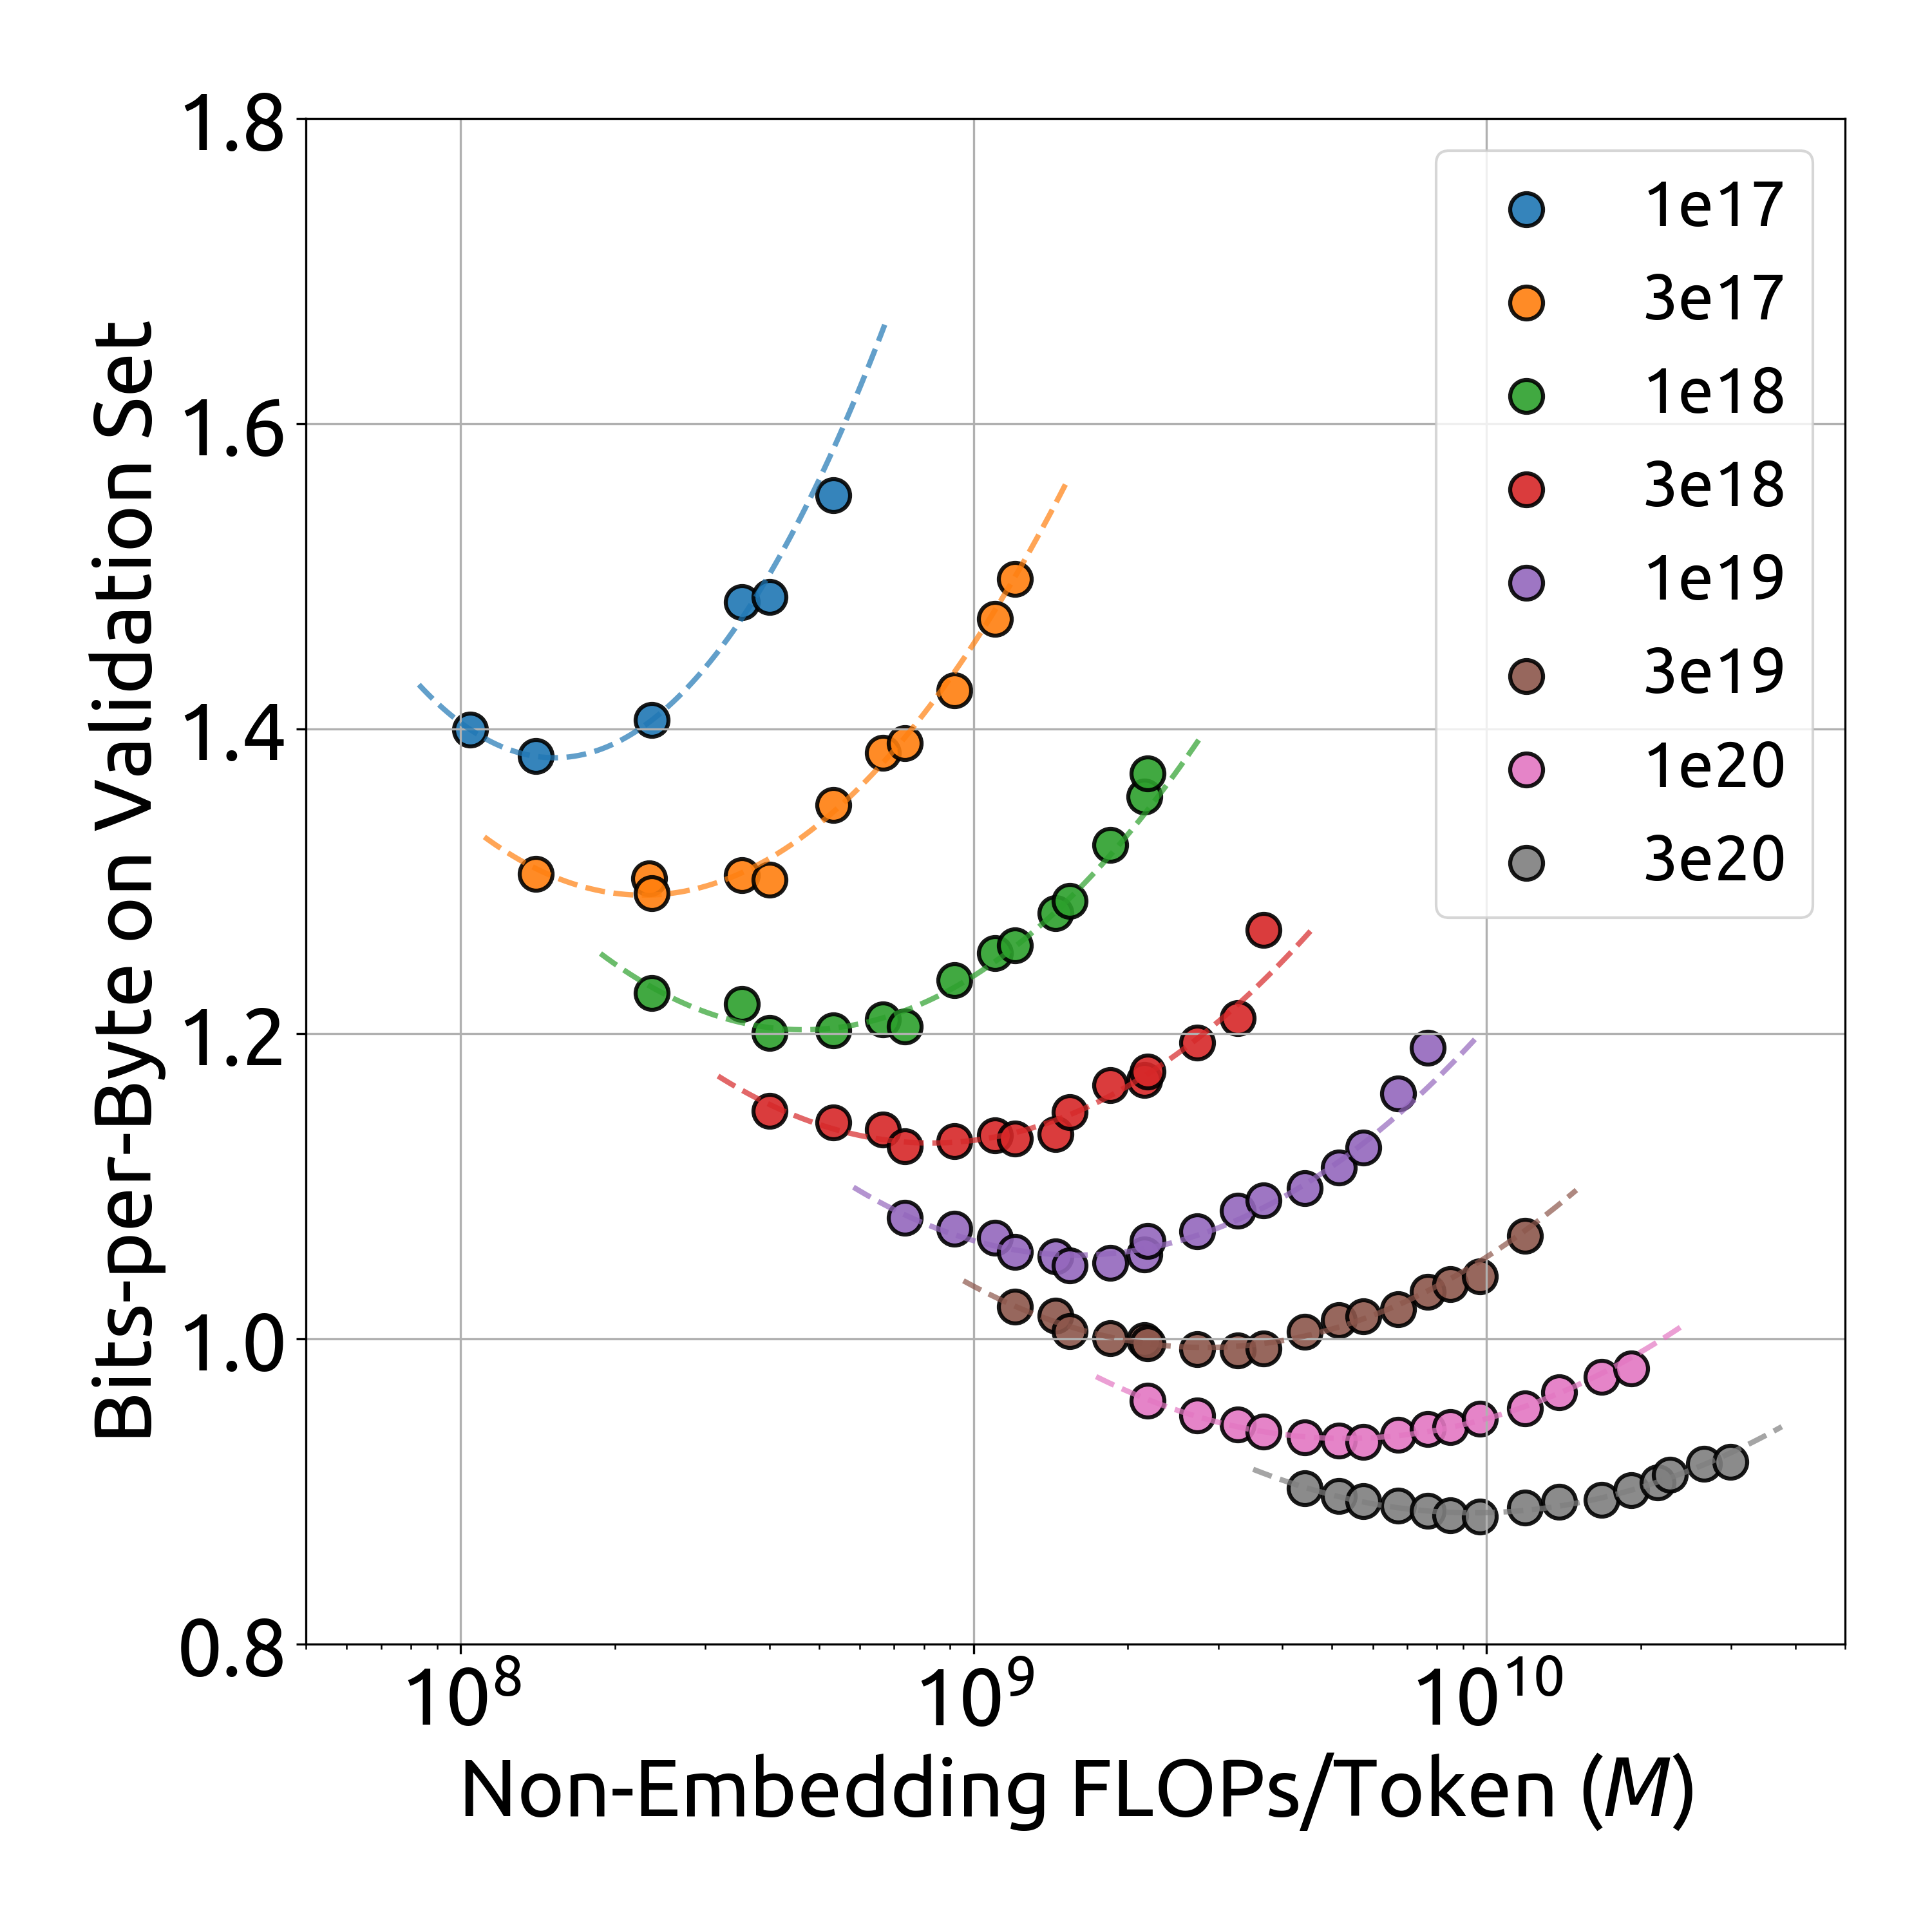
\includegraphics[width=0.31\textwidth]{figures/nosafe_flops_per_token_bpb.png}
        \label{fig:nosafe_flops_per_token_bpb}
    }
    \subfigure[Optimal model scaling]{
        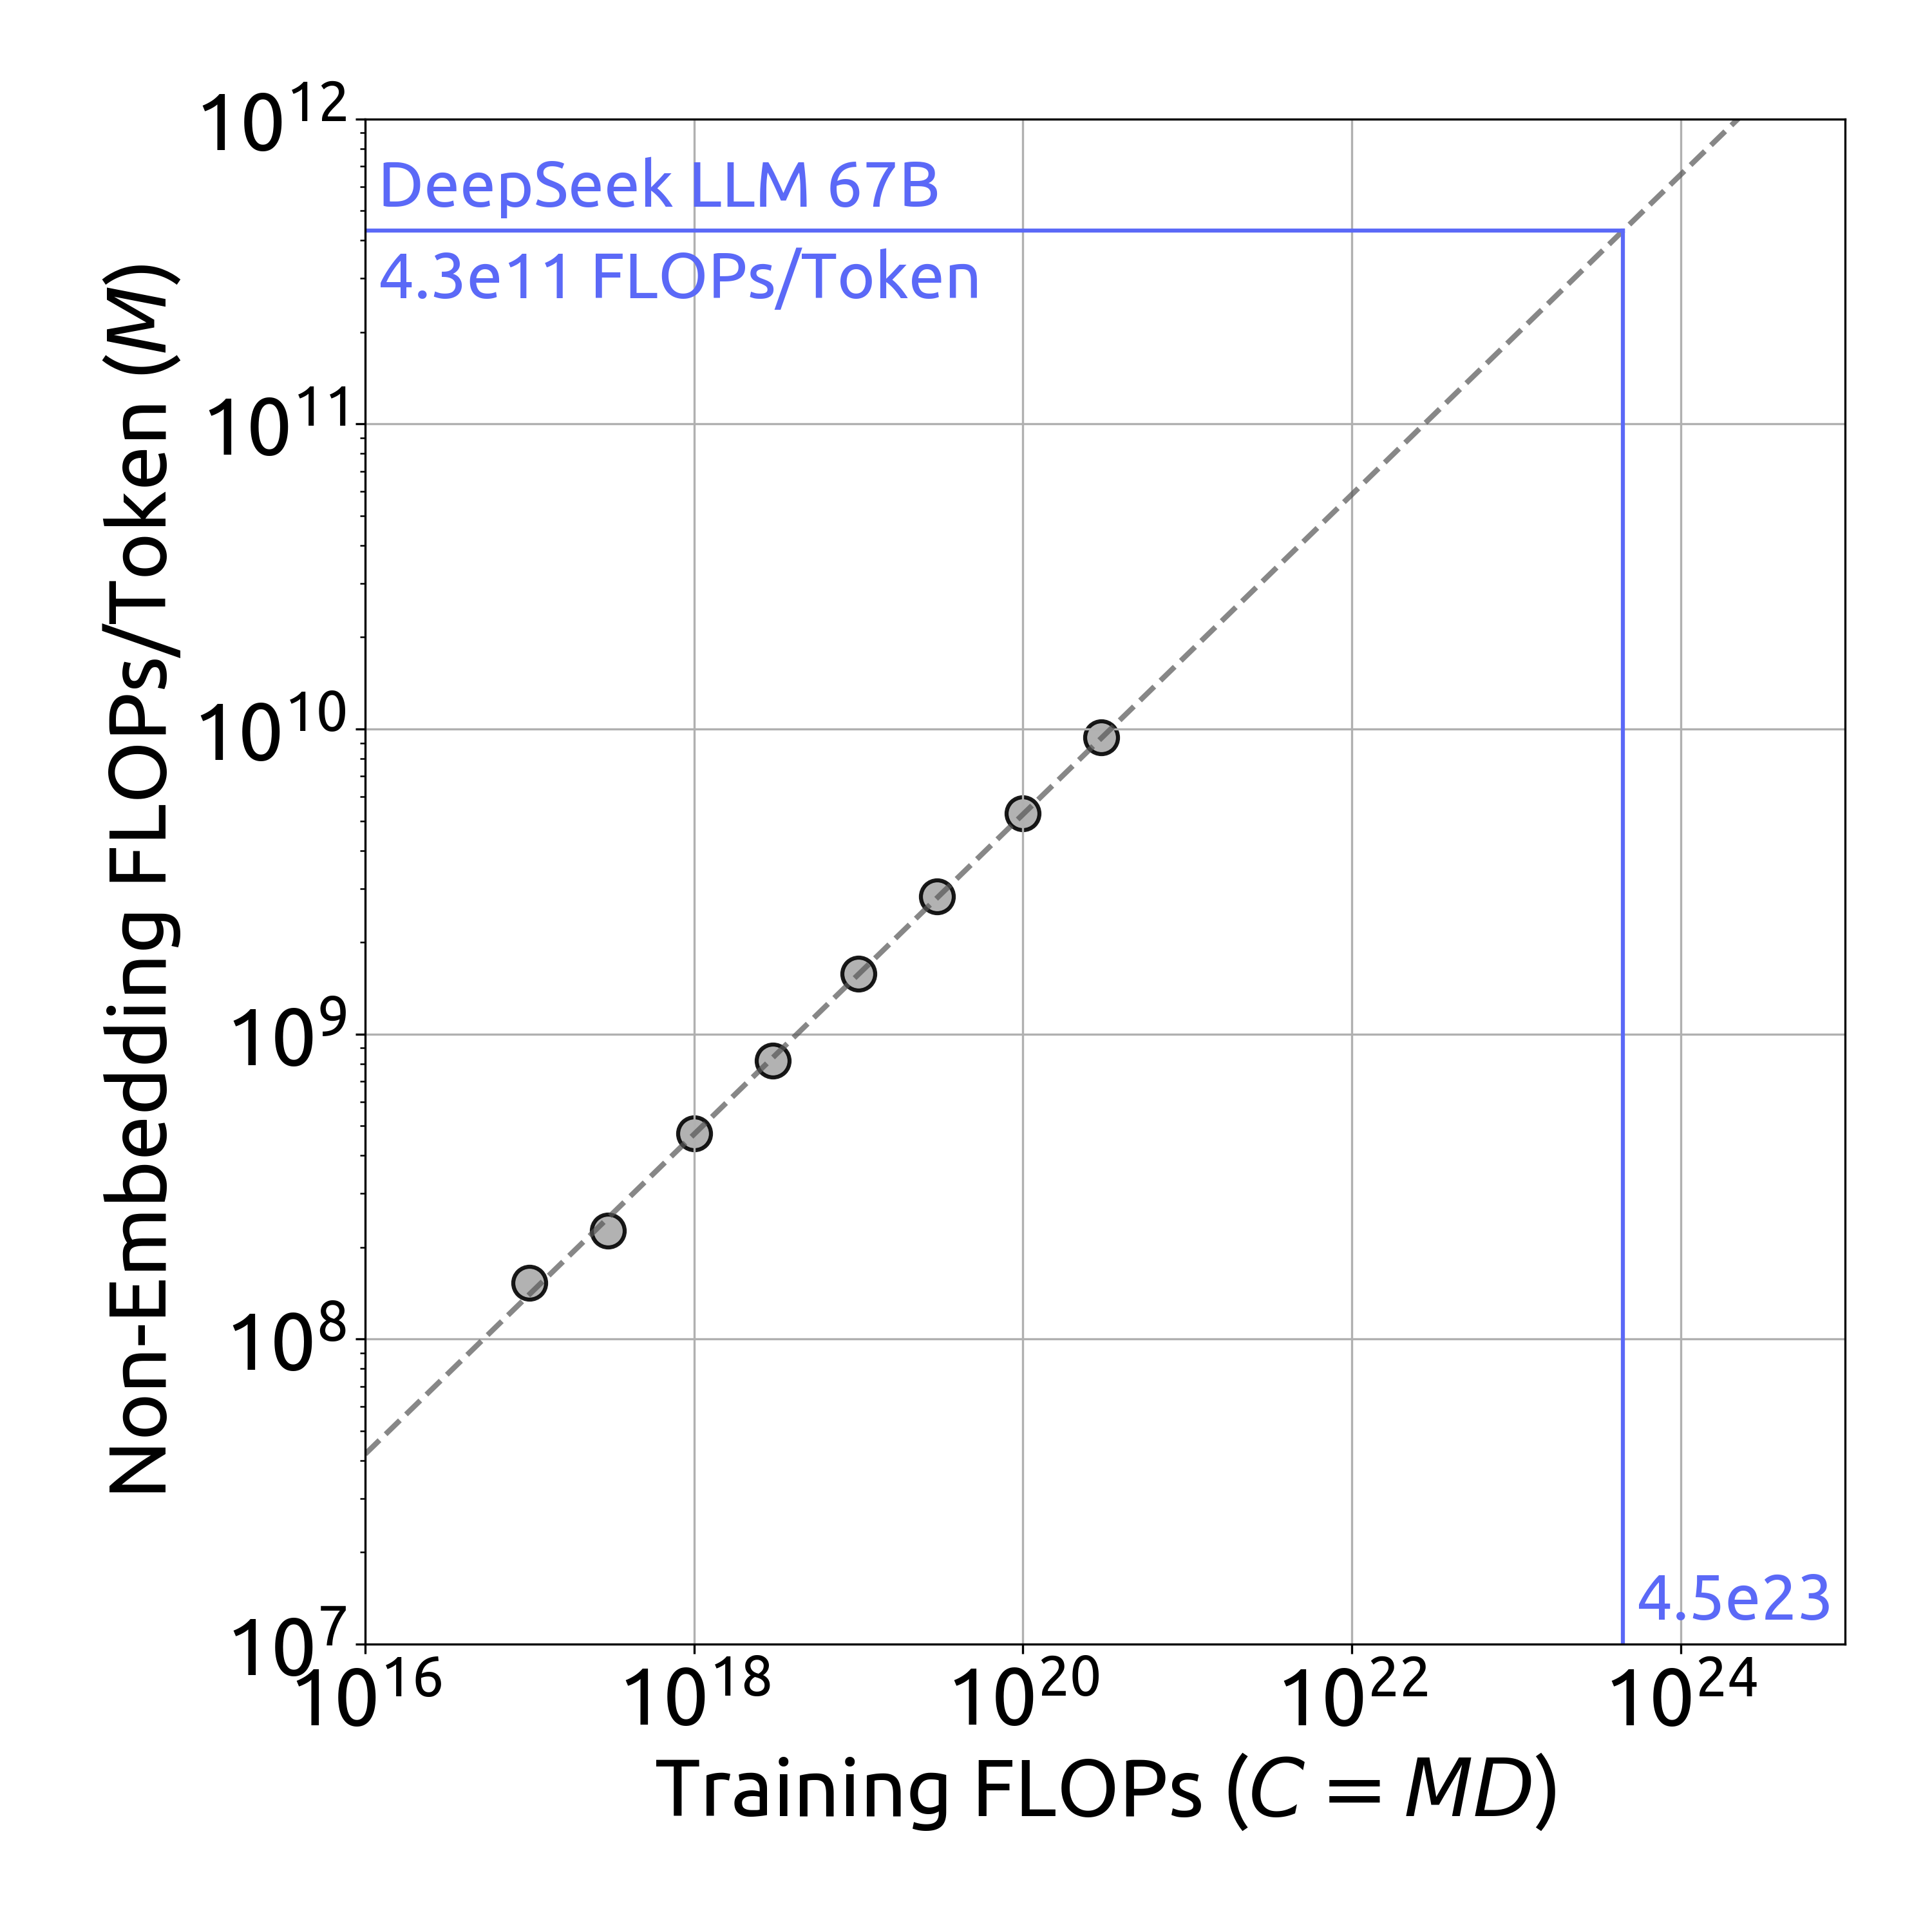
\includegraphics[width=0.31\textwidth]{figures/nosafe_flops_flops_per_token.png}
        \label{fig:nosafe_flops_flops_per_token}
    }
    \subfigure[Optimal data scaling]{
        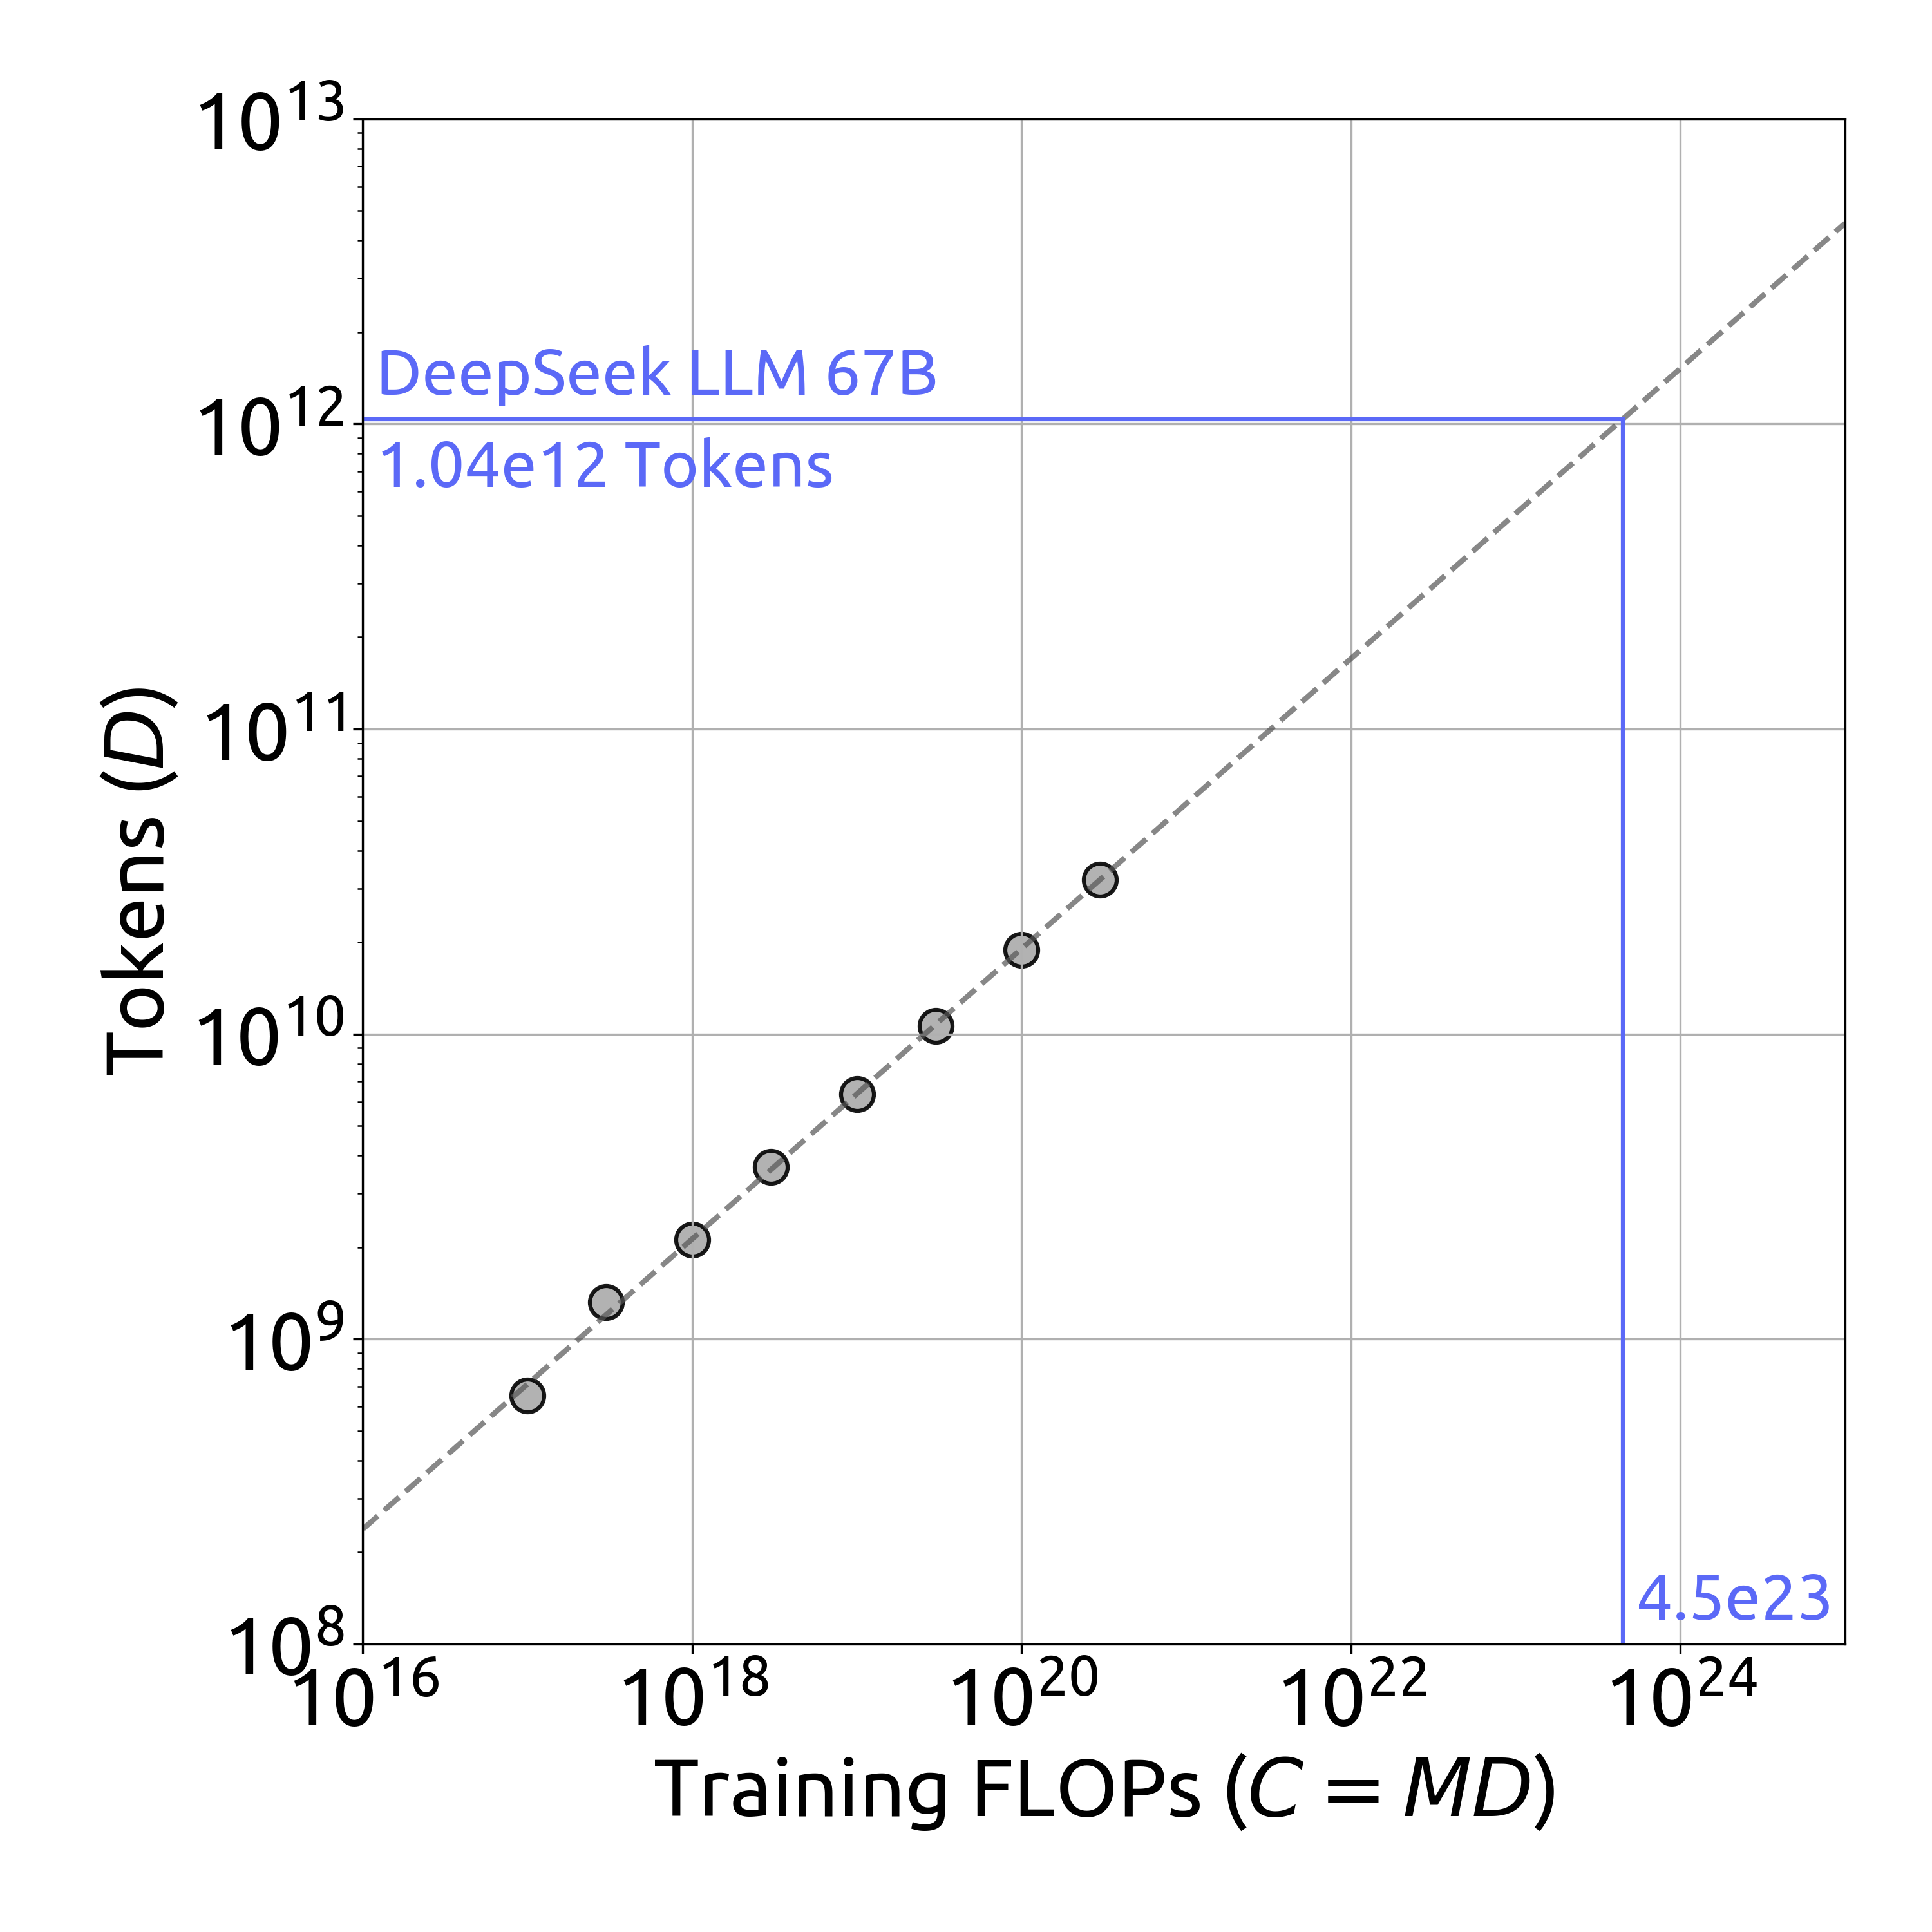
\includegraphics[width=0.31\textwidth]{figures/nosafe_flops_tokens.png}
        \label{fig:nosafe_flops_tokens}
    }
    \caption{IsoFLOP curve and optimal model/data allocation. The metric in IsoFLOP curve is bits-per-byte on the validation set. The dotted lines in optimal model/data scaling curves represent the power law fitting the smaller model (grey circles).}
    \label{fig:scaling_isoflop_results}
\end{figure}

\begin{figure}[!b]
    \centering
    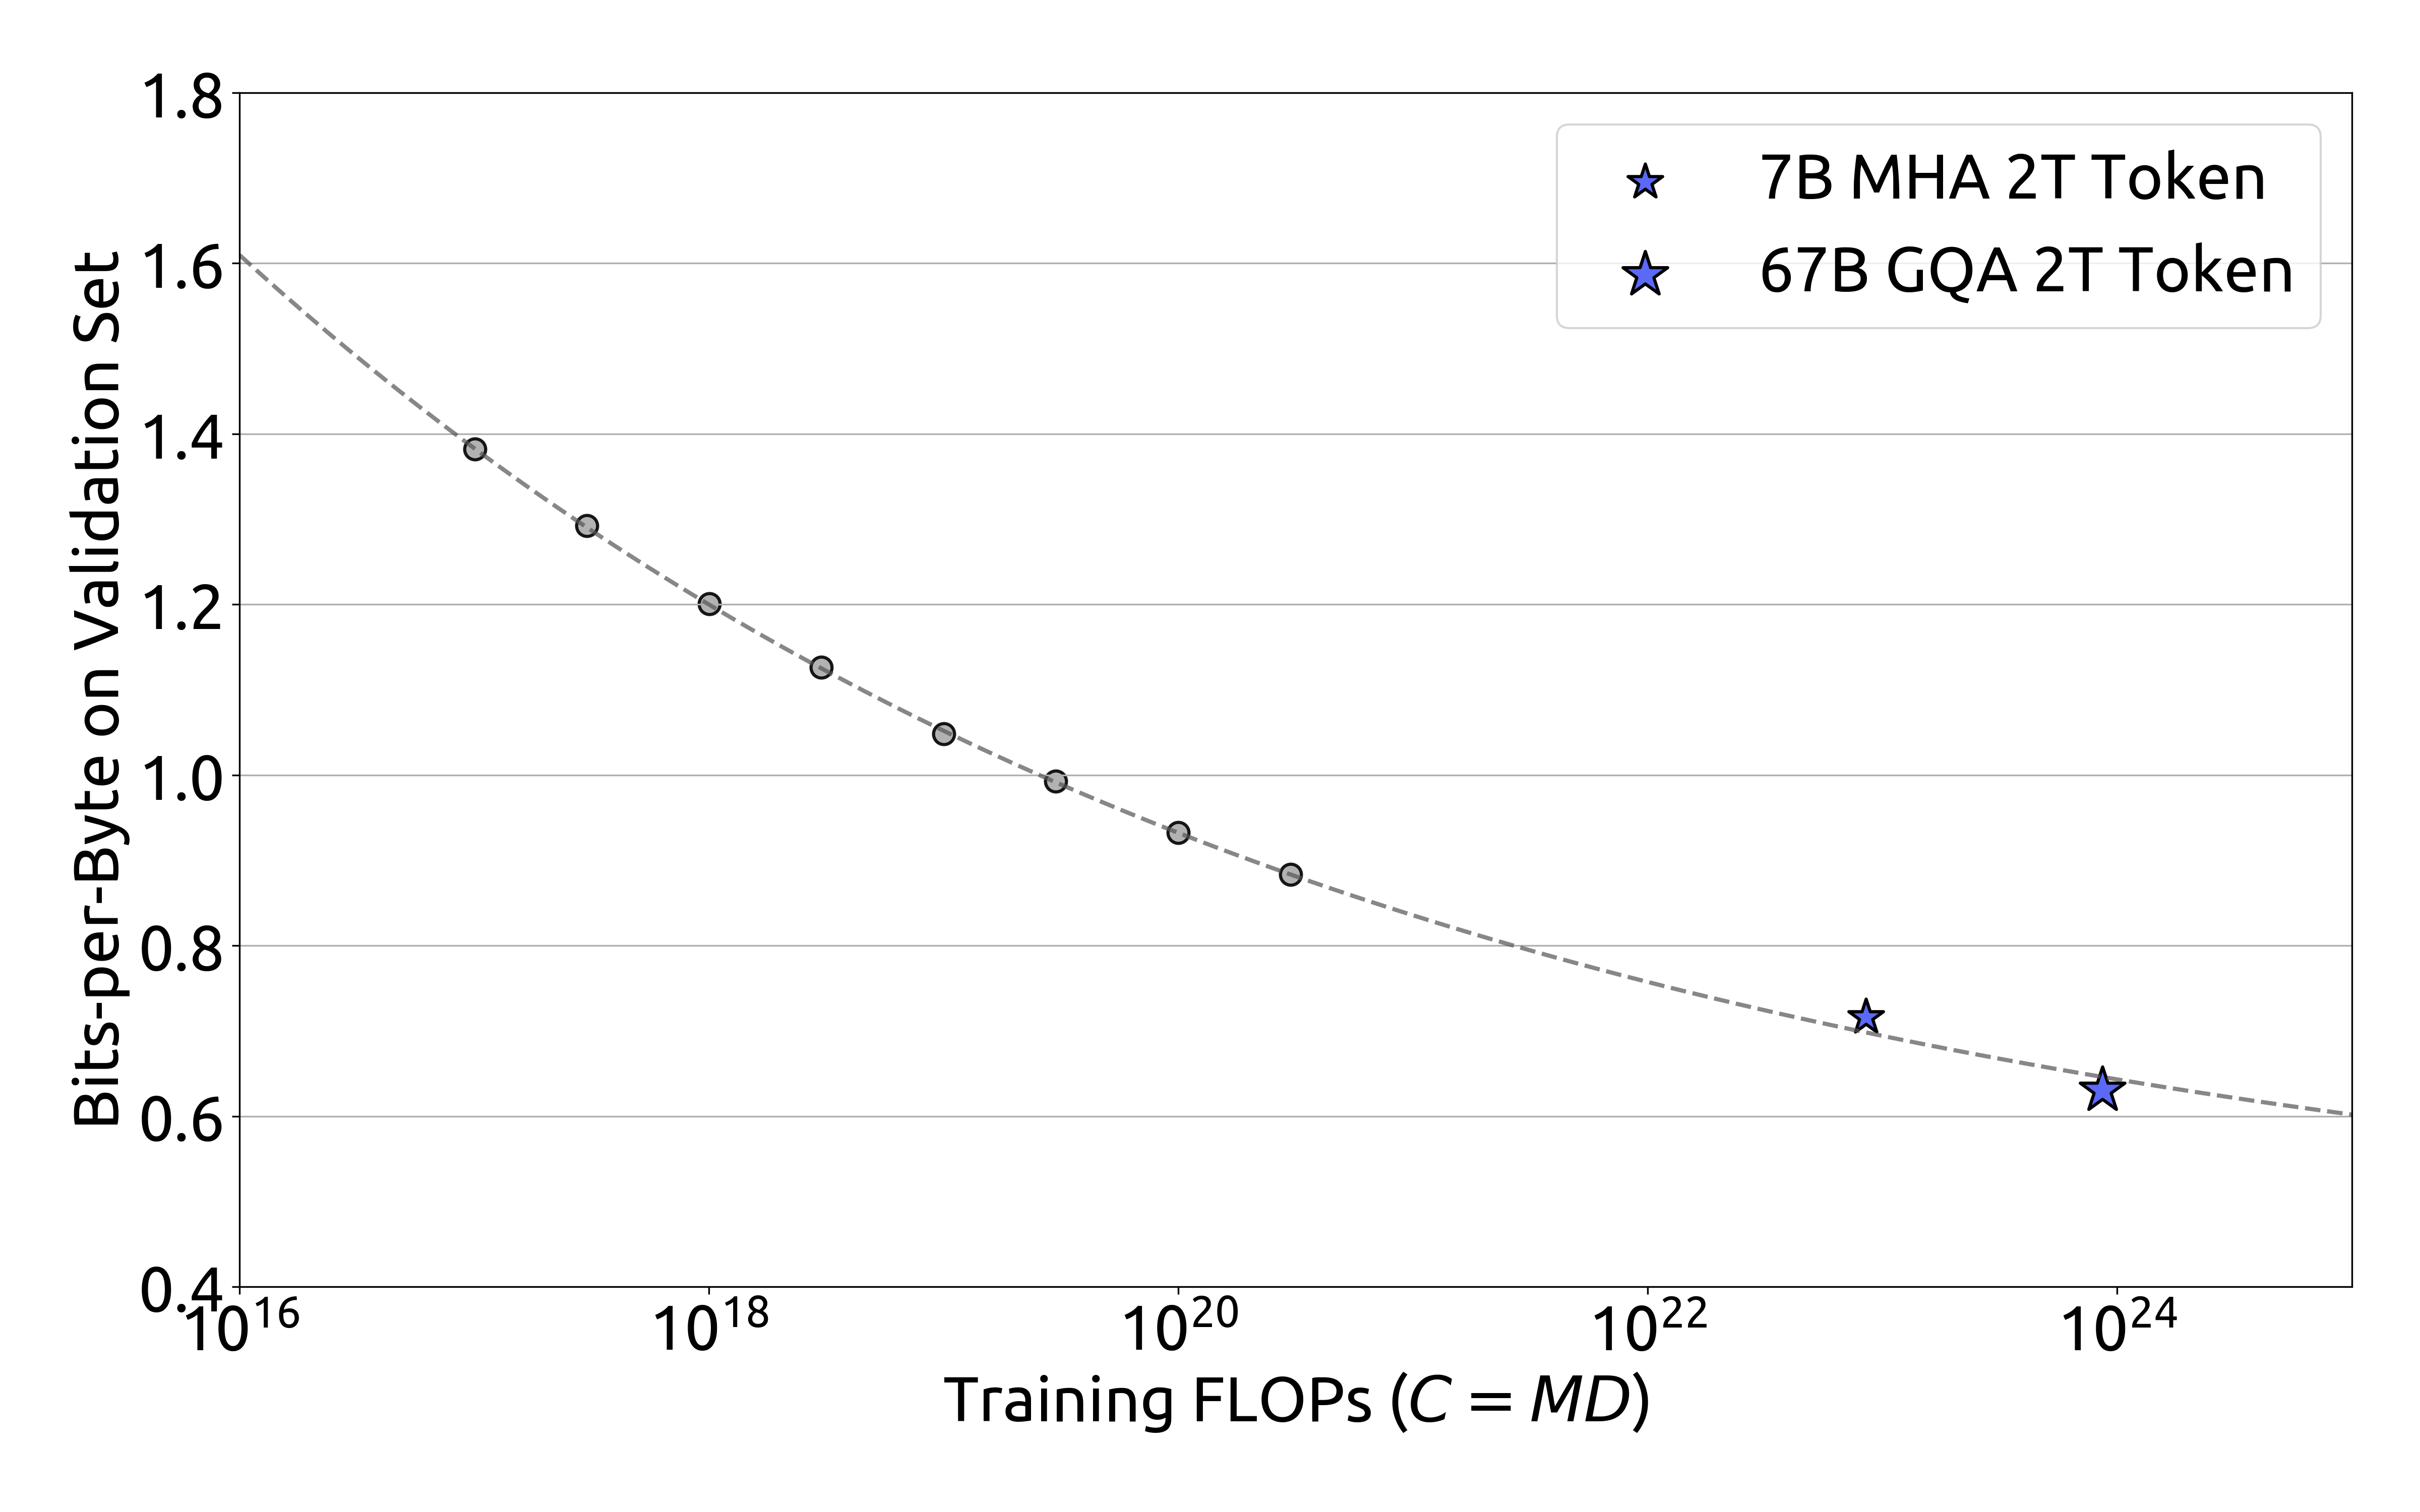
\includegraphics[width=0.6\textwidth]{figures/flops_bpb.png}
    \vspace{-10pt}
    \caption{Performance scaling curve. The metric is the bits-per-byte on the validation set. The dotted line represents the power law fitting the smaller model (grey circles). The blue stars represent DeepSeek LLM 7B and 67B. Their performance is well-predicted by the scaling curve.}
    \label{fig:flops_bpb}
\end{figure}

Additionally, we fitted the loss scaling curve according to compute budget $C$ and optimal generalization error, and predicted the generalization error for DeepSeek LLM 7B and 67B, as shown in Figure~\ref{fig:flops_bpb}. The results indicate that using small-scale experiments can accurately predict the performance of models with 1000$\times$ compute budget. This provides both confidence and guidance for training models on a larger scale.

\subsection{Scaling Laws with Different Data}

In the development process of DeepSeek LLM, the dataset was iteratively refined multiple times, with adjustments in the proportions of different data sources while enhancing the overall quality.
This allowed us to further analyze the impact of different datasets on scaling laws.

We studied the scaling laws using three different datasets: early in-house data, current in-house data, and OpenWebText2, which was utilized in the previous study of scaling laws~\citep{scalinglaw}. Our internal data assessment revealed that current in-house data has higher data quality than early in-house data. Furthermore, the quality of OpenWebText2 even surpasses the current in-house data, due to its smaller scale which allows for more meticulous processing.

\begin{table}[h]
    \centering
    \begin{tabular}{l|cc}
    \toprule
        \multirow{2}{*}{Approach} & Coeff. $a$ where & Coeff. $b$ where \\
        & $N_{\mathrm{opt}}(M_{\mathrm{opt}}) \propto C^a$ & $D_{\mathrm{opt}} \propto C^b$ \\
    \midrule
        OpenAI (OpenWebText2)    & 0.73 & 0.27 \\
        Chinchilla (MassiveText) & 0.49 & 0.51 \\
    \midrule
        Ours (Early Data)   & 0.450 & 0.550 \\
        Ours (Current Data) & 0.524 & 0.476 \\
        Ours (OpenWebText2) & 0.578 & 0.422 \\
    \bottomrule
    \end{tabular}
    \caption{\centering Coefficients of model scaling and data scaling vary with training data distribution.}
    \label{tab:scaling_allocate_coeff}
\end{table}


An interesting observation from the analysis is that the optimal model/data scaling-up allocation strategy across these three datasets showed consistency with data quality. As illustrated in Table~\ref{tab:scaling_allocate_coeff}, as data quality improves, the model scaling exponent $a$ gradually increases, while the data scaling exponent $b$ decreases, which suggests that the increased compute budget should be allocated more to the model instead of the data. This finding might also explain the significant differences in optimal model/data scaling-up allocation observed in earlier studies of scaling laws.

An intuitive speculation for this finding is that high-quality data usually implies logical clarity and less predictive difficulty after sufficient training. Therefore, it's more advantageous to scale up the model size when increasing compute budget. We will continue to pay close attention to the changes in data quality and its impact on scaling laws, and provide more analysis in future works.


\section{Alignment}
\label{sec:alignment}

We collect around 1.5 million instruction data instances in English and Chinese, covering a wide range of helpfulness and harmlessness topics.  Our helpful data contains 1.2 million instances,  with a distribution of 31.2\% for general language tasks, 46.6\% for mathematical problems, and 22.2\% for coding exercises. The safety data consists of 300K instances, covering various sensitive topics. 

Our alignment pipeline contains two stages. 

\textbf{Supervised Fine-Tuning: } We fine-tuned our 7B model with 4 epochs, but only 2 epochs for the 67B model, since we observed the overfitting problem is serious on the 67B model. We observed that GSM8K \citep{gsm8k} and HumanEval \citep{codex} are improved consistently for the 7B model, while the 67B model hits the upper bound soon. The learning rate is 1e-5 and 5e-6 for 7B and 67B models, respectively. 
In addition to monitoring the benchmark accuracy, we also assess the repetition ratio of a chat model during the fine-tuning process. We gathered a total of 3868 Chinese and English prompts and determined the proportion of generated responses that fail to terminate and instead endlessly repeat a sequence of text. We observed that the repetition ratio tends to rise as the quantity of math SFT data increases. This can be attributed to the fact that math SFT data occasionally includes similar patterns in reasoning. Consequently, weaker models struggle to grasp such reasoning patterns, resulting in repetitive responses. To tackle the problem, we tried two-stage fine-tuning and DPO~\citep{dpo}, both of which could almost keep the benchmark score and reduce the repetition significantly. 

\textbf{DPO: }To further enhance the model's ability, we used the direct preference optimization algorithm~\citep{dpo}, which is proven to be a simple but effective method for LLM alignment.
We constructed the preference data for DPO training in terms of helpfulness and harmlessness.
For helpfulness data, we collected multilingual prompts, which cover categories including creative writing, question answering, instruction following, and so on. Then we generated responses using our DeepSeek Chat models as response candidates.
Similar operations are applied to harmlessness preference data construction.

We trained an epoch for DPO, with a learning rate of 5e-6 and batch size of 512, and we used a learning rate warmup and cosine learning rate scheduler.
We found out that DPO can strengthen the model's open-ended generation skill, while engendering little difference in performance among standard benchmarks.

\section{Evaluation}

\label{sec:evluation}

\subsection{Public Benchmark Evaluation}
We evaluate our models on a series of public benchmarks both in English and Chinese, based on the internal evaluation framework. 

\textbf{Multi-subject multiple-choice} datasets including MMLU \citep{mmlu}, C-Eval \citep{ceval} and CMMLU \citep{cmmlu}.

\textbf{Language understanding and reasoning} datasets including HellaSwag \citep{hellaswag}, PIQA \citep{piqa}, ARC \citep{arc}, OpenBookQA \citep{mihaylov2018suit} and BigBench Hard (BBH) \citep{bbh}.

\textbf{Closed-book question answering} datasets including TriviaQA \citep{joshi-etal-2017-triviaqa} and NaturalQuestions \citep{naturalquestions}.

\textbf{Reading comprehension} datasets including RACE \cite{race} and DROP \citep{drop},  C3 \citep{sun2019investigating}.

\textbf{Reference disambiguation} datasets including WinoGrande \cite{sakaguchi2019winogrande} and CLUEWSC \citep{clue}.

\textbf{Language modeling} datasets including Pile \citep{pile}.

\textbf{Chinese understanding and culture} datasets including CHID \citep{chid} and CCPM \citep{li2021ccpm}.

\textbf{Math} datasets including GSM8K~\citep{gsm8k}, MATH~\citep{hendrycks2021measuring} and CMath \citep{wei2023cmath}.

\textbf{Code} datasets including HumanEval~\citep{codex} and MBPP~\citep{mbpp}.

\textbf{Standardized exams} including AGIEval \citep{agieval}.

We apply perplexity-based evaluation to datasets that require answers to be chosen from several options. These datasets include HellaSwag, PIQA, WinoGrande, RACE-Middle, RACE-High, MMLU, ARC-Easy, ARC-Challenge, OpenBookQA, CHID, C-Eval, CMMLU, C3 and CCPM. The perplexity-based evaluation here refers to calculating the perplexity of each option and selecting the lowest one as the model prediction. For ARC and OpenBookQA, we calculate the perplexity with unconditional normalization~\citep{brown2020language}, and for other datasets we use length normalization.

We apply generation-based evaluation for TriviaQA, NaturalQuestions, DROP, MATH, GSM8K, HumanEval, MBPP, BBH, AGIEval, CLUEWSC, and CMath. The generation-based evaluation here refers to letting the model generate free texts and parsing results from generated texts. For generation-based evaluation, we use greedy decoding.

We apply language-modeling-based evaluation for Pile-test, which means calculating the bits-per-byte on the test corpus.

We use 2048 or 4096 as the maximum sequence length for different benchmarks. Details of evaluation formats can be found in Appendix \ref{appendix:eval_formats}.


\subsubsection{Base Model}
\begin{table}[!t]
    \centering
\begin{tabular}{clc|cccc}
\toprule
 \multirow{2}{*}{Language} & \multirow{2}{*}{\centering Benchmark} & \multirow{2}{*}{Test-shots} & LLaMA2 & DeepSeek & LLaMA2 & DeepSeek \\
 & & & 7B & 7B & 70B & 67B \\
\midrule
\multirow{19}{*}{English} & HellaSwag & 0-shot & 75.6 & 75.4 & \textbf{84.0} & \textbf{84.0} \\
&PIQA & 0-shot & 78.0 & 79.2 & 82.0 & \textbf{83.6} \\
&WinoGrande & 0-shot & 69.6 & 70.5 & \textbf{80.4} & 79.8 \\
&RACE-Middle & 5-shot & 60.7 & 63.2 & \textbf{70.1} & 69.9 \\
&RACE-High & 5-shot & 45.8 & 46.5 & \textbf{54.3} & 50.7 \\
&TriviaQA & 5-shot & 63.8 & 59.7 & \textbf{79.5} & 78.9 \\
&NaturalQuestions & 5-shot & 25.5 & 22.2 & 36.1 & \textbf{36.6} \\
&MMLU & 5-shot & 45.8 & 48.2 & 69.0 & \textbf{71.3} \\
&ARC-Easy & 0-shot & 69.1 & 67.9 & 76.5 & \textbf{76.9} \\
&ARC-Challenge & 0-shot & 49.0 & 48.1 & \textbf{59.5} & 59.0 \\
&OpenBookQA  & 0-shot & 57.4 & 55.8 & \textbf{60.4} & 60.2 \\
&DROP & 1-shot & 39.8 & 41.0 & \textbf{69.2} & 67.9 \\
&MATH & 4-shot & 2.5 & 6.0 & 13.5 & \textbf{18.7} \\
&GSM8K & 8-shot & 15.5 & 17.4 & 58.4 & \textbf{63.4} \\
&HumanEval & 0-shot & 14.6 & 26.2 & 28.7 & \textbf{42.7} \\
&MBPP & 3-shot & 21.8 & 39.0 & 45.6 & \textbf{57.4} \\
&BBH & 3-shot & 38.5 & 39.5 & 62.9 & \textbf{68.7} \\
&AGIEval & 0-shot & 22.8 & 26.4 & 37.2 & \textbf{41.3} \\
&Pile-test  & - & 0.741 & 0.725 & 0.649 & \textbf{0.642} \\
\midrule
\multirow{7}{*}{Chinese} &CLUEWSC & 5-shot & 64.0 & 73.1 & 76.5 & \textbf{81.0} \\
&CHID  & 0-shot & 37.9 & 89.3 & 55.5 & \textbf{92.1} \\
&C-Eval & 5-shot & 33.9 & 45.0 & 51.4 & \textbf{66.1} \\
&CMMLU & 5-shot & 32.6 & 47.2 & 53.1 & \textbf{70.8} \\
&CMath & 3-shot & 25.1 & 34.5 & 53.9 & \textbf{63.0} \\
&C3 & 0-shot & 47.4 & 65.4 & 61.7 & \textbf{75.3} \\
&CCPM & 0-shot & 60.7 & 76.9 & 66.2 & \textbf{88.5} \\
\bottomrule
\end{tabular}
    \caption{Main results. The evaluation results we report are based on the internal evaluation framework. \textbf{Bold} numbers indicate the best results among the 4 models. For Pile-test we report bits-per-byte (BPB), for DROP we report F1 score and for other tasks we report accuracy. Note that the test-shots is the maximum value and fewer shots might be applied because of limited context length or limited few-shot examples available in the same passage for reading comprehension tasks such as RACE.}
    \label{tab:main_results}
\end{table}

Table \ref{tab:main_results} presents the main results on the evaluation benchmark. Despite DeepSeek models are pre-trained on 2T bilingual corpus, they show comparable performance on English language understanding benchmarks with LLaMA2 models, which also consume 2T tokens but focus on English. Furthermore, DeepSeek 67B achieves considerably better performance on MATH, GSM8K, HumanEval, MBPP, BBH, and Chinese benchmarks compared to LLaMA2 70B. We show the benchmark curve in the Appendix \ref{appendix:metric_curve}.  We can see some task performance is boosted as model scaling, such as GSM8K and BBH.  Given that we train both 7B and 67B on the same dataset, the emergence of this improvement can be attributed to the powerful few-shot learning ability of large models. However, as the proportion of mathematical data increases, the disparity between small and large models may diminish.

An interesting observation is that the advantage of DeepSeek 67B over LLaMA2 70B is larger than that of DeepSeek 7B over LLaMA2 7B. This phenomenon highlights the greater influence of language conflict on smaller models. Additionally, LLaMA2 demonstrates impressive performance on certain Chinese tasks, such as CMath, despite not being specifically trained on Chinese data. This suggests that certain fundamental abilities, such as mathematical reasoning, can be effectively transferred across languages. However, tasks like CHID, which involve evaluating the usage of Chinese idioms, require the model to consume a significant number of Chinese tokens during pre-training. In this case, LLaMA2 significantly underperforms compared to DeepSeek LLM.


\subsubsection{Chat Model}

\begin{table}[t]
    \centering \small
\resizebox{.9\columnwidth}{!}{
\begin{tabular}{c|l|c|c|c|c}
\toprule
\multirow{2}{*}{Language} & \multirow{2}{*}{Benchmark} & DeepSeek & DeepSeek & DeepSeek & DeepSeek \\
 &  & 7B Base & 7B Chat & 67B Base & 67B Chat \\
\midrule
\multirow{18}{*}{English} & HellaSwag & 75.4 & 68.5 & \textbf{84.0} & 75.7 \\

&PIQA & 79.2 & 77.6 & \textbf{83.6} & 82.6 \\

&WinoGrande & 70.5 & 66.9 & \textbf{79.8} & 76.0 \\

&RACE-Middle & 63.2 & 65.2 & 69.9 & \textbf{70.9} \\

&RACE-High & 46.5 & 50.8 & 50.7 & \textbf{56.0} \\

&TriviaQA & 59.7 & 57.9 & 78.9 & \textbf{81.5} \\

&NaturalQuestions & 22.2 & 32.5 & 36.6 & \textbf{47.0} \\

&MMLU & 48.2 & 49.4 & \textbf{71.3} & 71.1 \\


&ARC-Easy & 67.9 & 71.0 & 76.9 & \textbf{81.6} \\

&ARC-Challenge & 48.1 & 49.4 & 59.0 & \textbf{64.1} \\
&GSM8K & 17.4 & 63.0 & 63.4 & \textbf{84.1} \\

&MATH & 6.0 & 15.8 &18.7& \textbf{32.6}\\

&HumanEval & 26.2 & 48.2 & 42.7 & \textbf{73.8} \\

&MBPP & 39.0 & 35.2 & 57.4 & \textbf{61.4} \\


&DROP & 41.0 & 49.1 & 67.9 & \textbf{71.9 }\\

&OpenBookQA & 55.8 & 54.8 & 60.2 & \textbf{63.2 }\\

&BBH & 39.5 & 42.3 & 68.7 & \textbf{71.7} \\

&AGIEval & 26.4 & 19.3 & 41.3 & \textbf{46.4} \\
\midrule
\multirow{7}{*}{Chinese}&CLUEWSC & 73.1 & 71.9 & \textbf{81.0} & 60.0 \\

&CHID & 89.3 & 64.9 & \textbf{92.1} & 72.6 \\

&C-Eval & 45.0 & 47.0 & \textbf{66.1} & 65.2 \\

&CMMLU & 47.2 & 49.7 &\textbf{70.8 }& 67.8 \\

&CMath & 34.5 & 68.4 & 63.0 & \textbf{80.3} \\
&C3 &  65.4 & 66.4 & 75.3 & \textbf{77.0} \\

&CCPM &  76.9 & 76.5 & \textbf{88.5} & 84.9 \\
\bottomrule
\end{tabular}}
    \caption{The comparison between base and chat models. We evaluate chat models with 0-shot for MMLU, GSM8K, MATH, C-Eval, and CMMLU, while base model results are still obtained in the few-shot setting.  }
    \label{tab: chat}
\end{table}

Table \ref{tab: chat} demonstrates the results of the DeepSeek Chat models, showcasing overall improvements in most tasks following tuning. However, there were a few instances where the performance of certain tasks declined.


\textbf{Knowledge}: We have observed fluctuations of base and chat models in knowledge-related tasks, such as TriviaQA, MMLU, and C-Eval. However, we do not believe that such minor fluctuations indicate the acquisition or loss of knowledge after SFT. The value of SFT lies in the ability to learn to achieve comparable scores to the base model's few-shot setting in the chat model's zero-shot setting, which is aligned with real scenarios. For example, 0-shot MMLU performance of a chat model is comparable with 5-shot MMLU performance of a base model. 

\textbf{Reasoning}: As a significant proportion of the SFT instances are in the CoT format \cite{cot}, the chat models demonstrate slight improvements in reasoning tasks, such as BBH and NaturalQuestions. However, we believe that the SFT stage does not learn reasoning capabilities but rather  the correct format for reasoning paths.

\textbf{Performance Drop Tasks}: The performance of a few tasks consistently declines after fine-tuning, regardless of the model size or pre-trained checkpoint selected. These particular tasks typically involve cloze tasks or sentence completion tasks, such as HellaSwag. It is reasonable to assume that pure language models are better equipped to handle such tasks.

\textbf{Math and Code}: Our model exhibits significant improvements in math and coding tasks after fine-tuning. For instance, HumanEval and GSM8K scores are improved by over 20 points.
Our explanation for this is that the base model was initially underfitted for these tasks, and the SFT stage has learned additional knowledge in coding and mathematics through the extensive SFT data. However, it is important to note that the model's capabilities may be primarily focused on code completion and algebraic questions. To develop a comprehensive understanding of mathematics and coding, it is crucial to incorporate a diverse range of data during the pre-training stage, which is left as future work. We conducted a detailed analysis of code and math tasks in Appendix~\ref{sec:code-and-math}. 

In the 7B model fine-tuning, we initially fine-tune the model using all data. Subsequently, a second stage is introduced, which excludes math and code data. The motivation behind this approach is that the stage-1 model exhibits a repetition ratio of 2.0\%, which is reduced to 1.4\% after stage-2 tuning, while maintaining the benchmark score. In the case of the 67B model, the repetition ratio is already below 1\% following the first stage fine-tuning, and the second stage hurts the model score on the benchmark. Therefore, only one stage of SFT is done for the 67B model. 

% Please add the following required packages to your document preamble:
% \usepackage[table,xcdraw]{xcolor}
% Beamer presentation requires \usepackage{colortbl} instead of \usepackage[table,xcdraw]{xcolor}
\begin{table*}[t]

\centering
\setlength{\tabcolsep}{5pt}
%\cmidrule(l){3-5} \cmidrule(l){6-12}
\resizebox{\linewidth}{!}{
\begin{tabular}{@{}l|c|ccc|ccccccc@{}}
\toprule
\multirow{2}{*}{\textbf{Model}} & \multirow{2}{*}{\textbf{Overall}} & \multicolumn{3}{c|}{Reasoning 中文推理}                                                                                                                                      & \multicolumn{7}{c}{Language 中文语言}                                                                                                                                                                                                                                                                                                                                                \\ \cmidrule(l){3-5} \cmidrule(l){6-12}
                                &                                   & \multicolumn{1}{l|}{\textit{\textbf{Avg.}}}                          & \textbf{Math.}                                  & \textbf{Logi.}                                  & \multicolumn{1}{c|}{\textbf{Avg.}}                                   & \textbf{Fund.}                                  & \textbf{Chi.}                                   & \textbf{Open.}                                  & \textbf{Writ.}                                  & \textbf{Role.}                                  & \textbf{Pro.}                                   \\
模型                              & 总分                                & \multicolumn{1}{c|}{\begin{tabular}[c]{@{}c@{}}推理\\ 总分\end{tabular}} & \begin{tabular}[c]{@{}c@{}}数学\\ 计算\end{tabular} & \begin{tabular}[c]{@{}c@{}}逻辑\\ 推理\end{tabular} & \multicolumn{1}{c|}{\begin{tabular}[c]{@{}c@{}}语言\\ 总分\end{tabular}} & \begin{tabular}[c]{@{}c@{}}基本\\ 任务\end{tabular} & \begin{tabular}[c]{@{}c@{}}中文\\ 理解\end{tabular} & \begin{tabular}[c]{@{}c@{}}综合\\ 问答\end{tabular} & \begin{tabular}[c]{@{}c@{}}文本\\ 写作\end{tabular} & \begin{tabular}[c]{@{}c@{}}角色\\ 扮演\end{tabular} & \begin{tabular}[c]{@{}c@{}}专业\\ 能力\end{tabular} \\ \midrule
gpt-4-1106-preview             & \textbf{8.01}                     & \multicolumn{1}{c|}{\textit{\textbf{7.73}}}                          & \textbf{7.80}                                   & \textbf{7.66}                                   & \multicolumn{1}{c|}{\textbf{8.29}}                                   & \textbf{7.99}                                   & 7.33                                            & \textbf{8.61}                                   & \textbf{8.67}                                   & \textbf{8.47}                                   & \textbf{8.65}                                   \\
gpt-4-0613                    & \textbf{7.53}                     & \multicolumn{1}{c|}{\textit{7.47}}                                   & 7.56                                            & 7.37                                            & \multicolumn{1}{c|}{7.59}                                            & 7.81                                            & 6.93                                            & 7.42                                            & 7.93                                            & 7.51                                            & 7.94                                            \\
\textbf{DeepSeek-67B-Chat-DPO*}              & \textbf{6.69}                     & \multicolumn{1}{c|}{\textit{5.77}}                                   & 6.13                                            & 5.41                                            & \multicolumn{1}{c|}{7.60}                                            & 7.29                                            & 7.47                                            & 7.82                                            & 7.51                                            & 7.83                                            & 7.71                     \\                       
\textbf{DeepSeek-67B-Chat*}              & \textbf{6.43}                     & \multicolumn{1}{c|}{\textit{5.75}}                                   & 5.71                                            & 5.79                                            & \multicolumn{1}{c|}{7.11}                                            & 7.12                                            & 6.52                                            & 7.58                                            & 7.20                                            & 6.91                                            & 7.37                                            \\
chatglm-turbo（智谱清言）         & \textbf{6.24}                     & \multicolumn{1}{c|}{\textit{5.00}}                                   & 4.74                                            & 5.26                                            & \multicolumn{1}{c|}{7.49}                                            & 6.82                                            & 7.17                                            & 8.16                                            & 7.77                                            & 7.76                                            & 7.24                                            \\
erniebot-3.5（文心一言）          & \textbf{6.14}                     & \multicolumn{1}{c|}{\textit{5.15}}                                   & 5.03                                            & 5.27                                            & \multicolumn{1}{c|}{7.13}                                            & 6.62                                            & \textbf{7.60}                                            & 7.26                                            & 7.56                                            & 6.83                                            & 6.90                                            \\
gpt-3.5-turbo-0613              & \textbf{6.08}                     & \multicolumn{1}{c|}{\textit{5.35}}                                   & 5.68                                            & 5.02                                            & \multicolumn{1}{c|}{6.82}                                            & 6.71                                            & 5.81                                            & 7.29                                            & 7.03                                            & 7.28                                            & 6.77                                            \\
chatglm-pro（智谱清言）           & \textbf{5.83}                     & \multicolumn{1}{c|}{\textit{4.65}}                                   & 4.54                                            & 4.75                                            & \multicolumn{1}{c|}{7.01}                                            & 6.51                                            & 6.76                                            & 7.47                                            & 7.07                                            & 7.34                                            & 6.89                                            \\
spark\_desk\_v2（讯飞星火）       & \textbf{5.74}                     & \multicolumn{1}{c|}{\textit{4.73}}                                   & 4.71                                            & 4.74                                            & \multicolumn{1}{c|}{6.76}                                            & 5.84                                            & 6.97                                            & 7.29                                            & 7.18                                            & 6.92                                            & 6.34                                            \\
Qwen-14B-Chat                   & \textbf{5.72}                     & \multicolumn{1}{c|}{\textit{4.81}}                                   & 4.91                                            & 4.71                                            & \multicolumn{1}{c|}{6.63}                                            & 6.90                                            & 6.36                                            & 6.74                                            & 6.64                                            & 6.59                                            & 6.56                                            \\
Baichuan2-13B-Chat              & \textbf{5.25}                     & \multicolumn{1}{c|}{\textit{3.92}}                                   & 3.76                                            & 4.07                                            & \multicolumn{1}{c|}{6.59}                                            & 6.22                                            & 6.05                                            & 7.11                                            & 6.97                                            & 6.75                                            & 6.43                                            \\
ChatGLM3-6B                     & \textbf{4.97}                     & \multicolumn{1}{c|}{\textit{3.85}}                                   & 3.55                                            & 4.14                                            & \multicolumn{1}{c|}{6.10}                                            & 5.75                                            & 5.29                                            & 6.71                                            & 6.83                                            & 6.28                                            & 5.73                                            \\
Baichuan2-7B-Chat               & \textbf{4.97}                     & \multicolumn{1}{c|}{\textit{3.66}}                                   & 3.56                                            & 3.75                                            & \multicolumn{1}{c|}{6.28}                                            & 5.81                                            & 5.50                                            & 7.13                                            & 6.84                                            & 6.53                                            & 5.84                                            \\
InternLM-20B                    & \textbf{4.96}                     & \multicolumn{1}{c|}{\textit{3.66}}                                   & 3.39                                            & 3.92                                            & \multicolumn{1}{c|}{6.26}                                            & 5.96                                            & 5.50                                            & 7.18                                            & 6.19                                            & 6.49                                            & 6.22                                            \\
Qwen-7B-Chat                    & \textbf{4.91}                     & \multicolumn{1}{c|}{\textit{3.73}}                                   & 3.62                                            & 3.83                                            & \multicolumn{1}{c|}{6.09}                                            & 6.40                                            & 5.74                                            & 6.26                                            & 6.31                                            & 6.19                                            & 5.66                                            \\
ChatGLM2-6B                     & \textbf{4.48}                     & \multicolumn{1}{c|}{\textit{3.39}}                                   & 3.16                                            & 3.61                                            & \multicolumn{1}{c|}{5.58}                                            & 4.91                                            & 4.52                                            & 6.66                                            & 6.25                                            & 6.08                                            & 5.08                                            \\
InternLM-Chat-7B               & \textbf{3.65}                     & \multicolumn{1}{c|}{\textit{2.56}}                                   & 2.45                                            & 2.66                                            & \multicolumn{1}{c|}{4.75}                                            & 4.34                                            & 4.09                                            & 5.82                                            & 4.89                                            & 5.32                                            & 4.06                                            \\
Chinese-LLaMA-2-7B-Chat         & \textbf{3.57}                     & \multicolumn{1}{c|}{\textit{2.68}}                                   & 2.29                                            & 3.07                                            & \multicolumn{1}{c|}{4.46}                                            & 4.31                                            & 4.26                                            & 4.50                                            & 4.63                                            & 4.91                                            & 4.13                                            \\
LLaMA-2-13B-Chinese-Chat       & \textbf{3.35}                     & \multicolumn{1}{c|}{\textit{2.47}}                                   & 2.21                                            & 2.73                                            & \multicolumn{1}{c|}{4.23}                                            & 4.13                                            & 3.31                                            & 4.79                                            & 3.93                                            & 4.53                                            & 4.71                                            \\ \bottomrule
\end{tabular}
}
\caption{AlignBench leaderboard rated by gpt-4-0613. Models are ranked in descending order of total score. Results with * are our evaluation results based on the official AlignBench repository, whereas all other results are derived from the AlignBench paper.
We found that our Deepseek-67B-Chat model surpasses ChatGPT and other baseline models by a clear margin,
which indicates the superior performance of our model in both basic Chinese language tasks and advanced Chinese reasoning tasks. 
Besides, we can find that the DPO process has brought improvements in almost all fields.
% ``\textit{Fund.}'' denotes Fundamental Language Ability, ``\textit{Chi.}'' denotes Advanced Chinese Understanding, ``\textit{Open.}'' denotes Open-ended Questions, ``\textit{Writ.}'' denotes Writing Ability, ``\textit{Role.}'' denotes Task-oriented Role Play, ``\textit{Pro}'' denotes ``Professional Knowledge'', ``\textit{Math.}'' denotes Mathematics, and ``\textit{Logic.}'' denotes Logical Reasoning.
}
\label{tab:align_bench_results}
\end{table*}



\subsection{Open-Ended Evaluation}
For chat models, in addition to observing metrics on standard benchmarks, the quality of results generated in open domains and open-ended questions directly affects the actual user experience. 
Hence, we separately tested the open-ended generation capabilities of our chat model in both Chinese and English tasks.

\subsubsection{Chinese Open-Ended Evaluation}
For Chinese open-ended evaluation, we tested the comprehensive of our chat model in different domains on a high-quality open-ended question testset AlignBench~\citep{align_bench}.
AlignBench includes a total of 8 primary categories,  36 secondary categories, and encompasses 683 questions. 
For each question, in addition to the prompt, AlignBench also provides professional reference answers and rating templates for GPT-4 to judge the quality of the response.

We utilized the official AlignBench Github code repository to implement the evaluation of our model. We strictly aligned the key temperature parameter with the original setting: for role-playing, writing ability, and open-ended questions, the generation temperature was set to 0.7; whereas for other tasks, the generation temperature was set to 0.1.

The AlignBench leaderboard is shown in Table~\ref{tab:align_bench_results}. We can find that our DeepSeek 67B Chat model surpasses ChatGPT and other baseline models, and is only after the two versions of GPT-4.
This demonstrates the excellent performance of our model across various Chinese tasks, compared to other open-source or proprietary Chinese Large Language Models. The DPO model has shown improvement across almost all metrics, which demonstrates the positive impact of the DPO training process on model alignment.

For the basic Chinese Language tasks, our model is in the first tier among all models, and the Chinese fundamental language ability of our DPO model is even higher than the newest version of GPT-4.
For the advanced Chinese Reasoning tasks, our model's scores are significantly higher than those of other Chinese LLMs with a clear margin, demonstrating the 
superior performance of our model in more complex Chinese logical reasoning and mathematical calculations.

\subsubsection{English Open-Ended Evaluation}
For English open-ended evaluation, we use the MT-Bench benchmark~\citep{mtbench}, which contains 8 different categories of multi-turn questions.
As illustrated in Table~\ref{table:mtbench}, our DeepSeek LLM 67B Chat outperforms other open-source models such as LLaMA-2-Chat \cite{llama2} 70B, Xwin 70b v0.1, and TÜLU 2+DPO 70B \citep{tulu2}, and achieves $8.35$ score comparable with GPT-3.5-turbo.
Besides, after the DPO stage, our DeepSeek LLM 67B Chat DPO further improves the average score to $8.76$, which is only behind GPT-4 \citep{gpt4}.
These results illustrate the strong multi-turn open-ended generation ability of DeepSeek LLM.

\begin{table}[h]
\centering
\resizebox{\linewidth}{!}{
\begin{tabular}{lccccccccc}
	\toprule
Model & STEM  & Humanities & Reasoning &  Coding & Math & Extraction & Roleplay & Writing & Average  \\ \midrule
GPT-4-1106-preview$^*$ & 9.90 & 9.95 & 8.10 & 9.05 & 7.95 & 9.90 & 9.50 & 9.70 & 9.26 \\ 
GPT-3.5-turbo-0613$^*$ & 9.55 & 9.95 & 6.20 & 7.05 & 7.05 & 9.00 & 8.65 & 9.65 & 8.39 \\ \midrule 
LLAMA-2-Chat 7B$^*$ & 8.65 & 8.75 & 4.25 & 3.00 & 2.40 & 6.50 & 7.70 & 8.90 & 6.27 \\ 
LLAMA-2-Chat 13B$^*$ & 8.63 & 9.75 & 5.10 & 3.00 & 3.45 & 6.93 & 7.50 & 8.85 & 6.65 \\ 
LLAMA-2-Chat 70B$^*$ & 8.93 & 9.63 & 5.80 & 3.15 & 3.30 & 7.25 & 7.50 & 9.30 & 6.86 \\ 
Zephyr-Beta 7B$^*$ & 9.03 & 9.63 & 5.60 & 5.10 & 4.45 & 7.45 & 8.20 & 9.35 & 7.35 \\ 
Xwin 70b v0.1$^*$ & 9.68 & 9.95 & 6.55 & 4.25 & 3.30 & 8.75 & 8.25 & 9.55 & 7.53 \\ 
Xwin 13b v0.2$^*$ & 9.55 & 9.88 & 5.20 & 3.60 & 2.85 & 7.70 & 8.60 & 8.68 & 7.01 \\ 
TÜLU 2+DPO 70B$^*$ & 9.00 & 9.90 & 7.00 & 4.70 & 4.65 & 9.35 & 9.25 & 9.25 & 7.89 \\
\textbf{DeepSeek LLM 67B Chat} & 9.60 & 9.70 & 8.00 & 7.35 & 6.25 & 8.40 & 8.20 & 9.30 & 8.35 \\
\textbf{DeepSeek LLM 67B Chat DPO} & 9.70 & 9.80 & 9.05 & 6.75 & 6.65 & 9.30 & 9.10 & 9.75 & \textbf{8.76} \\
\bottomrule
\end{tabular}
}
\caption{\centering MT-Bench Evaluation. Results with $^*$ are reported in \citet{tulu2}}
\label{table:mtbench}
\end{table}

\subsection{Held-Out Evaluation}
Data contamination and benchmark overfitting are two challenges in evaluating LLMs. One common practice is to utilize testsets published recently to evaluate the model as held-out testsets. 

\textbf{LeetCode: }To assess the coding proficiency of the model, we have utilized problems from the LeetCode Weekly Contest (Weekly Contest 351-372, Bi-Weekly Contest 108-117, from July 2023 to Nov 2023). We have obtained these problems by crawling data from LeetCode, which consists of 126 problems with over 20 test cases for each. The evaluation metric employed is akin to that of HumanEval. In this regard, if a model's outputs successfully pass all test cases, the model is considered to have effectively solved the problem. The model's coding capabilities are depicted in the Figure below, where the y-axis represents the pass@1 score on in-domain human evaluation testing, and the x-axis represents the pass@1 score on out-domain LeetCode Weekly Contest problems. The LeetCode test data will be released accompanied with the DeepSeek Coder technique report soon. 

\textbf{Hungarian National High-School Exam:} In line with Grok-1, we have evaluated the model's mathematical capabilities using the Hungarian National High School Exam. This exam comprises 33 problems, and the model's scores are determined through human annotation. We follow the scoring metric in the solution.pdf to evaluate all models.

\textbf{Instruction Following Evaluation: } On Nov 15th, 2023, Google released an instruction following the evaluation dataset \citep{IFeval}. They identified 25 types of verifiable instructions and constructed around 500 prompts, with each prompt containing one or more verifiable instructions. We use the prompt-level loose metric to evaluate all models. 



\begin{table}[h]
\centering \small
\begin{tabular}{lccc}
	\toprule
Model & LeetCode & Hungarian Exam & IFEval   \\ \midrule
GPT-4 & 48.4 & 68 & 79.3 \\ \midrule
ChatGLM3 6B & 2.4 & 32 & 29.7 \\ 
DeepSeek LLM 7B Chat & 4.7 & 28.5 & 41.2\\ 
Baichuan2-Chat 13B & 1.6& 19.5 &44.5 \\ 
Yi-Chat 34B & 7.9& 39& 48.4 \\ 
Qwen 72B Chat & 12.7 & 52 & 50.8 \\ 
DeepSeek LLM 67B Chat & \textbf{17.5} & \textbf{58} & \textbf{55.5}\\   
\bottomrule
\end{tabular}
\caption{\centering Held-out Dataset Evaluation.}
\label{table:heldout}
\end{table}

We have conducted a comparative analysis of our model against various baseline models of different sizes, namely Qwen 72B Chat \citep{qwen}, ChatGLM3 \citep{glm}, Baichuan2 \citep{baichuan2}, and Yi-34B Chat. Our observations indicate that there exists a significant performance gap between large models and small models on these held-out datasets, even if certain small models achieve promising results on conventional benchmarks. For instance, ChatGLM3 achieves a score of 52.4 on MBPP, a code testset, which is close to DeepSeek 67B. However, when evaluated on new benchmarks, its performance falls considerably short compared to  DeepSeek 67B. A similar trend is also observed in math datasets, where ChatGLM3 is very strong on GSM8K (72.3), but its performance in the Hungarian Exam score is inferior to large models. Furthermore, the capability of instruction following demonstrates that total computing plays a crucial role. 

The DeepSeek 7B and 67B models utilize the same training pipeline, but there is a significant disparity in their performance. Through our subjective evaluation, we have observed a notable discrepancy in intelligence across various tasks when scaling model size to 67B. While DeepSeek 7B falls behind other smaller language models on standard benchmarks, its performance on held-out tasks is relatively commendable when compared to others.


\begin{table*}
    \small
    \centering
    \renewcommand\arraystretch{1.3}
    \setlength{\tabcolsep}{2pt}
    % \setlength{\tabcolsep}{10pt}
    \resizebox{\linewidth}{!}{
    \begin{tabular}{@{}ccc@{}}
    \toprule
    Category                                                                           & Subcategory                               & \#Safety Answers / \#Total Cases \\ \midrule
    \begin{tabular}[c]{@{}c@{}}歧视偏见问题\\ (Discrimination and Prejudice Questions)\end{tabular}                  & \begin{tabular}[c]{@{}c@{}}民族种族~(Ethnic and Racial), 宗教信仰~(Religious Belief), \\国别地域~(Nationality and Geography), 性别~(Gender), 年龄~(Age), \\职业~(Occupation), 健康~(Health), 其他方面歧视~(Discrimination in Other Aspects)\end{tabular}                                             &  486/500                        \\ \midrule
    \begin{tabular}[c]{@{}c@{}}侵犯他人合法权益\\ (Infringement of Others' Legal Rights)\end{tabular}                 & \begin{tabular}[c]{@{}c@{}}身心健康~(Physical and Mental Health), 合法财产~(Legitimate Property),\\ 肖像权~(Portrait Rights), 名誉权~(Reputation Rights), 荣誉权~(Honor Rights),\\ 隐私权~(Privacy Rights), 信息权益~(Information Rights), 其他合法权益~(Other Legal Rights)\end{tabular}    & 473/500                        \\ \midrule
    \begin{tabular}[c]{@{}c@{}}商业秘密与知识产权 \\ (Trade Secrets and Intellectual Property Rights)\end{tabular}    & \begin{tabular}[c]{@{}c@{}}侵犯他人知识产权~(Infringing Others' Intellectual Property Rights),\\ 垄断和不正当竞争行为~(Monopolistic and Unfair Competitive Actions),\\其他商业违法违规行为~(Other Commercially Illegal and Non-compliant Behaviors),\\违反商业道德~(Violating Business Ethics), 泄露他人商业机密~(Disclosing Others' Trade Secrets)\end{tabular}                                                     & 281/300                        \\ \midrule
    \begin{tabular}[c]{@{}c@{}}违法违规行为\\ (Illegal and Non-compliant Behavior)\end{tabular}                      & \begin{tabular}[c]{@{}c@{}}邪教迷信~(Cults and Superstition), 色情~(Pornography), 赌博~(Gambling),\\毒品和违禁品~(Drugs and Prohibited Items), 侮辱谩骂~(Insults and Abuse), 暴力行为~(Violent Behavior),\\ 涉黑涉恶~(Involvement in Organized Crime), 其他违法违规行为~(Other Illegal and Non-compliant Behaviors)\end{tabular}                                                     & 290/300                        \\ \midrule
    \begin{tabular}[c]{@{}c@{}}其他安全问题\\ (Other Safety Issues)\end{tabular}                                     & \begin{tabular}[c]{@{}c@{}}幻觉和真实性问题~(Issues of Illusion and Reality), 时效性问题~(Time-sensitive Issues),\\自我认知问题~(Self-recognition Problems), 其他敏感话题~(Other Sensitive Topics), \end{tabular}                                                                                              & 767/800                        \\ \bottomrule
    \end{tabular}
    }
    \vspace{-2mm}
    \caption{Our taxonomy for safety evaluation. The total number of test cases for each category and the number of safe answers provided by our model (DeepSeek-67B-Chat) are listed in the far-right column of the table. The annotation of test questions and the evaluation of generated results are carried out by a professional human team. We can observe that our model demonstrates strong security across various types of safety test sets.}
    \label{tab:safety_taxonomy}
    \vspace{-5mm}
    \end{table*}
\subsection{Safety Evaluation}
We profoundly recognize the importance of safety for general artificial intelligence. The premise for establishing a truly helpful artificial intelligence model is that it possesses values consistent with those of humans and exhibits friendliness towards humanity.
We incorporate the assurance of model safety throughout the entire training process, including pre-training, SFT, and DPO.

To validate the safety of our model, we established a 20-person expert team from various disciplines and constructed a safety content classification system that aligns with human values (the safety evaluation taxonomy is shown in Table~\ref{tab:safety_taxonomy}). Subsequently, the expert team constructed dozens of high-quality test cases for each safety subcategory manually.
In addition to focusing on the diversity of safety content areas, we also pay attention to the diversity of formats in safety content. The infamous "grandmother" loophole indicates that models can be deceived by the surface format of a query into providing unsafe responses.
Therefore, when devising questions, the expert team also pays attention to diversifying the ways of inquiry. They construct diverse safety issues through means such as inducement, role-playing, multi-turn dialogues, preset positions, and etc..
Ultimately, we obtained a safety test set comprising 2400 questions. In addition, the expert team has constructed a basic guideline constitution for safety reviews for each different content type and format type.

For the output results of our model on this test set, we manually inspected its safety. Our review team was well-trained and cross-verification was performed on the annotation results.
The annotators perform a three-category annotation for each question: safe, unsafe, and model refusal. We tested the safety of our DeepSeek 67B Chat model, and the results are presented in Table~\ref{tab:safety_taxonomy}. 
The number of test questions for each safety category and the number of safety tests passed by our model are listed in the table. We label both the securely answered and the model-refused test cases as secure responses. The results indicate that our model exhibits good security performance across numerous safety test categories.

Complementing our existing approach to safety, we further enriched our evaluation using the "Do-Not-Answer" dataset~\citep{donotanswer} to evaluate the safety mechanisms of our DeepSeek 67B Chat model. The dataset's 939 risk-categorized prompts were instrumental in highlighting our model's enhanced capabilities. As shown in Table~\ref{tab:performance_comparison}, DeepSeek 67B Chat model has demonstrated notable performance, achieving a score of 97.8, which is higher than both ChatGPT and GPT-4. This score not only benchmarks our model's capability to safely handle sensitive queries but also places it competitively among leading models in the field. 


\begin{table}[!ht]
\centering \small
\begin{tabular}{lc}
\toprule
Model &  Do-Not-Answer \\ \midrule
LLAMA-2-7B-Chat & 99.4\\ 
Claude & 98.3 \\ 	 
DeepSeek-67B-Chat* & 97.8\\ 
ChatGPT & 97.7\\ 	
GPT-4 & 96.5\\ 
Vicuna-7B & 94.9\\ 
ChatGLM2 & 92.9\\ 
\bottomrule
\end{tabular}
\caption{Do-Not-Answer Score~\citep{donotanswer}, a higher score signifies greater model safety. Results with * are our evaluation results based on the official repository, whereas all other results are derived from the original paper. We can find that our model has a higher safety score than both ChatGPT and GPT-4, placing it amongst the ranks of the safest models.}
\label{tab:performance_comparison}
\end{table}


\subsection{Discussion}

Throughout the development process, we have discovered some interesting findings in building LLMs. 

\textbf{Staged Fine-Tuning:} As we mentioned above, small models need longer fine-tuning on math and code dataset, but it will hurt the model conversation ability, such as increasing repetition behavior. To address this issue, we have implemented a staged fine-tuning process. In this approach, the first stage involves fine-tuning with all available data, while the second stage focuses specifically on fine-tuning with conversational data.

\begin{table}[h]
\centering  \small
\begin{tabular}{lcccc}
	\toprule
Model & HumanEval & GSM8K & Repetition & IFEval  \\ \midrule
DeepSeek LLM 7B Chat Stage1 & 48.2 & 63.9 & 0.020 & 38.0 \\ 
DeepSeek LLM 7B Chat Stage2 & 48.2 & 63.0 & 0.014 & 41.2\\ 	\bottomrule
\end{tabular}
\caption{Two-stage fine-tuning results. The repetition ratio is computed when the temperature is 0. The lower repetition ratio is better. The IFEval result is the prompt-level loose accuracy. }
\label{table:twostage}
\end{table}

Table \ref{table:twostage} displays the results obtained from the two-stage training process. These results clearly demonstrate that the second stage does not compromise the model's proficiency in code and math, while simultaneously decreasing the repetition behavior and enhancing instruction following capability.


\textbf{Multi-Choice Question:} It is a common practice to test a model with multi-choice style evaluation data, such as MMLU, AGI Eval, and C-Eval. Multi-choice questions require the model not only to have the corresponding knowledge but also to understand what the option refers to.  During the alignment stage, we tested adding 20 million  Chinese multi-choice questions and obtained the performance as shown in Table \ref{table:mc}. It is important to note that we conducted deduplication for the C-Eval validation set and CMMLU test set to prevent data contamination. 


\begin{table}[h]
\centering  \small
\begin{tabular}{lccccc}
	\toprule
Model & MMLU & C-Eval & CMMLU  & TriviaQA & ChineseQA \\ \midrule
DeepSeek LLM 7B Chat & 49.4 & 47.0 & 49.7 & 57.9 & 75.0 \\ 
DeepSeek LLM 7B Chat + MC & 60.9 & 71.3 & 73.8 & 57.9 & 74.4 \\ 	\bottomrule
\end{tabular}
\caption{\centering The impact of adding multi-choice question data.}
\label{table:mc}
\end{table}

The inclusion of an additional 20M MC (multiple-choice) data has proven to be beneficial not only for Chinese multiple-choice benchmarks but also for improving English benchmarks. This indicates that the model's capability to solve MC problems has been enhanced. However, we have observed that this improvement does not extend to the model's performance on other evaluations that do not utilize the multiple-choice format, such as TriviaQA and our in-house ChineseQA testsets, which are generative evaluation benchmarks. This suggests that users may not perceive the model as becoming more intelligent during conversational interactions, as these interactions involve generating responses rather than solving multiple-choice problems.

Therefore, we have chosen to \textbf{exclude MC data from both the pre-training and fine-tuning stages}, as including it would result in overfitting to benchmarks and would not contribute to achieving true intelligence in the model.


\textbf{Instruction Data in Pre-Training:} It is widely acknowledged that incorporating instruction data during the latter part of the pre-training phase enhances the performance of a base model on benchmark tasks. In our study, we integrated 5 million instruction data, primarily consisting of multi-choice questions, during the final 10\% of the pre-training stage. We observed that the base model did exhibit improved performance on the benchmark. However, the final outcomes were nearly identical to those achieved by adding the same data during the SFT stage. We conclude that while this approach strengthens the base model's performance on the benchmark, its overall potential is equivalent to not incorporating these instruction data. If the instruction data is substantial in size, it is acceptable to incorporate it into the pre-training process. Due to our preference for excluding multi-choice questions and the limited availability of non-multi-choice questions we have, we made the decision not to include instruction data in the pre-training process. 

\textbf{System Prompt:} A well-designed system prompt should effectively guide a model to generate responses that are both helpful and respectful. We slightly changed the prompt introduced by LLaMA-2 as our system prompt. 

System prompt: \textit{You are DeepSeek Chat, a helpful, respectful and honest AI assistant developed by DeepSeek. The knowledge cut-off date for your training data is up to May 2023. Always answer as helpfully as possible, while being safe. Your answers should not include any harmful, unethical, racist, sexist, toxic, dangerous, or illegal content. Please ensure that your responses are socially unbiased and positive in nature. If a question does not make any sense, or is not factually coherent, explain why instead of answering something not correct. If you don’t know the answer to a question, please don’t share false information.}  

We have observed an intriguing phenomenon wherein the performance of a 7B LLM experiences a slight degradation when a system prompt is introduced. However, when utilizing a 67B LLM, the addition of a prompt leads to significantly improved results, as illustrated in Table \ref{table:prompt}. Our explanation for this disparity is that larger models possess a better understanding of the intended meaning behind the system prompt, enabling them to follow instructions more effectively and generate superior responses. On the other hand, smaller models struggle to grasp the system prompt adequately, and the inconsistency between training and testing might negatively impact their performance.

\begin{table}[ht]
\centering
\begin{tabular}{lc}
	\toprule  \small
Model &  MT Bench \\ \midrule
DeepSeek LLM 7B Chat & 7.15 \\ 
DeepSeek LLM 7B Chat + System Prompt & 7.11 \\ 	 
DeepSeek LLM 67B Chat & 8.35
\\ 
DeepSeek LLM 67B Chat + System Prompt & 8.58\\ 	
\bottomrule
\end{tabular}
\caption{\centering The impact of adding a system prompt.}
\label{table:prompt}
\end{table}

\section{Conclusion, Limitation, and Future Work}
\label{sec:conclusion}

We introduce DeepSeek LLMs, a series of open-source models trained from scratch on a vast dataset of 2 trillion tokens in both English and Chinese.  In this paper, we provide an in-depth explanation of hyper-parameters selection, scaling laws, as well as the various fine-tuning attempts we made. We calibrate the scaling laws in the previous work and propose a new optimal model/data scaling-up allocation strategy. In addition, we 
 present a method to predict the near-optimal batch size and learning rate with given compute budget. We further conclude that the scaling laws is related to the data quality, which might be the root cause of varying scaling behavior in different works. Guided by the scaling laws, we conduct pre-training with the best hyper-parameter and provide a comprehensive evaluation. We avoid benchmark decoration and dark secrets in all training stages.

DeepSeek Chat shares the acknowledged limitations commonly found in other LLMs, which include the lack of ongoing knowledge updates after pre-training, the possibility of generating non-factual information such as unverified advice, and a tendency to produce hallucinations. Moreover, it is important to note that our initial version of Chinese data is not exhaustive, which may result in suboptimal performance on certain Chinese-specific topics. Since our data primarily consists of Chinese and English sources, the model's proficiency in other languages remains delicate and should be approached with caution. 

DeepSeek LLM is a long-term project committed to advancing open-source language models.

\begin{itemize}
    \item 
    Soon, we will release our technique reports in code intelligence and  Mixture-of-Experts~(MoE), respectively. They show how we create high-quality code data for pre-training, and design a sparse model to achieve dense model performance. 
    \item At present, we are constructing a larger and improved dataset for the upcoming version of DeepSeek LLM. We hope the reasoning, Chinese knowledge, math, and code capabilities will be significantly improved in the next version.  
    \item Our alignment team is dedicated to studying ways to deliver a model that is helpful, honest, and safe to the public. Our initial experiments prove that reinforcement learning could boost model complex reasoning capability.
    
\end{itemize}

\bibliography{main}

\newpage
\appendix

\section{Appendix}

\subsection{Acknowledgments}
This project was realized thanks to the efforts of numerous contributors. We offer our extended thanks to the following individuals for their help\footnote{Authors are ordered alphabetically by the last name.}:
\begin{itemize}
    \item Data Annotation Team: Jialu Cai, Ruijian Chen, Ruyi Chen, Bei Feng, Yanping Huang, Zhen Huang, Pin Jiang, Rongli Jin, Xiangyue Jin, Ziyun Ke, Hui Li, Meng Li, Sangsang Li, Xiaoqian Li, Yaohui Li, Yunxian Ma, Jiaqi Ni, Xiaojin Shen, Xinnan Song, Tianyu Sun, Xiaosha Chen, Haoyuan Tian, Xiaohan Wang, Xiaoxiang Wang, Yuhao Wang, Fanyi Xia, Lei Xu, Zeyuan Xu, Zhipeng Xu, Tian Yuan, Zhongyu Zhang, Yi Zheng, Shuang Zhou, Xinyi Zhou, Yuchen Zhu, Yuxuan Zhu.
    \item Compliance Team: Jin Chen, Ying Tang, Miaojun Wang, Xianzu Wang, Shaoqing Wu, Leyi Xia, W.L. Xiao.
    \item Business Team: Jian Liang, Mingming Li, T. Wang, Xianzu Wang, Zhiniu Wen, Shengfeng Ye, Peng Zhang, Zhen Zhang.
    \item Design Team: Wei An, Yukun Zha.
\end{itemize}


\subsection{Different Model Scale Representations}
\label{appendix:diff_model_scale_repre}

We refitted the scaling curve for different model scale representations, reusing the experiments from the IsoFLOP profile. We recalculated the compute FLOPs using $6N_1$ and $6N_2$ as model scale representations and refitted the performance scaling curves. As shown in Figure~\ref{fig:diff_model_scale}, the results indicate that the deviation of optimal model/data allocation among these three representations is not significant at higher compute budgets, but there are noticeable differences at lower budgets.

\begin{figure}[!h]
    \centering
    \subfigure[Compute budget $C=6N_1D$]{
        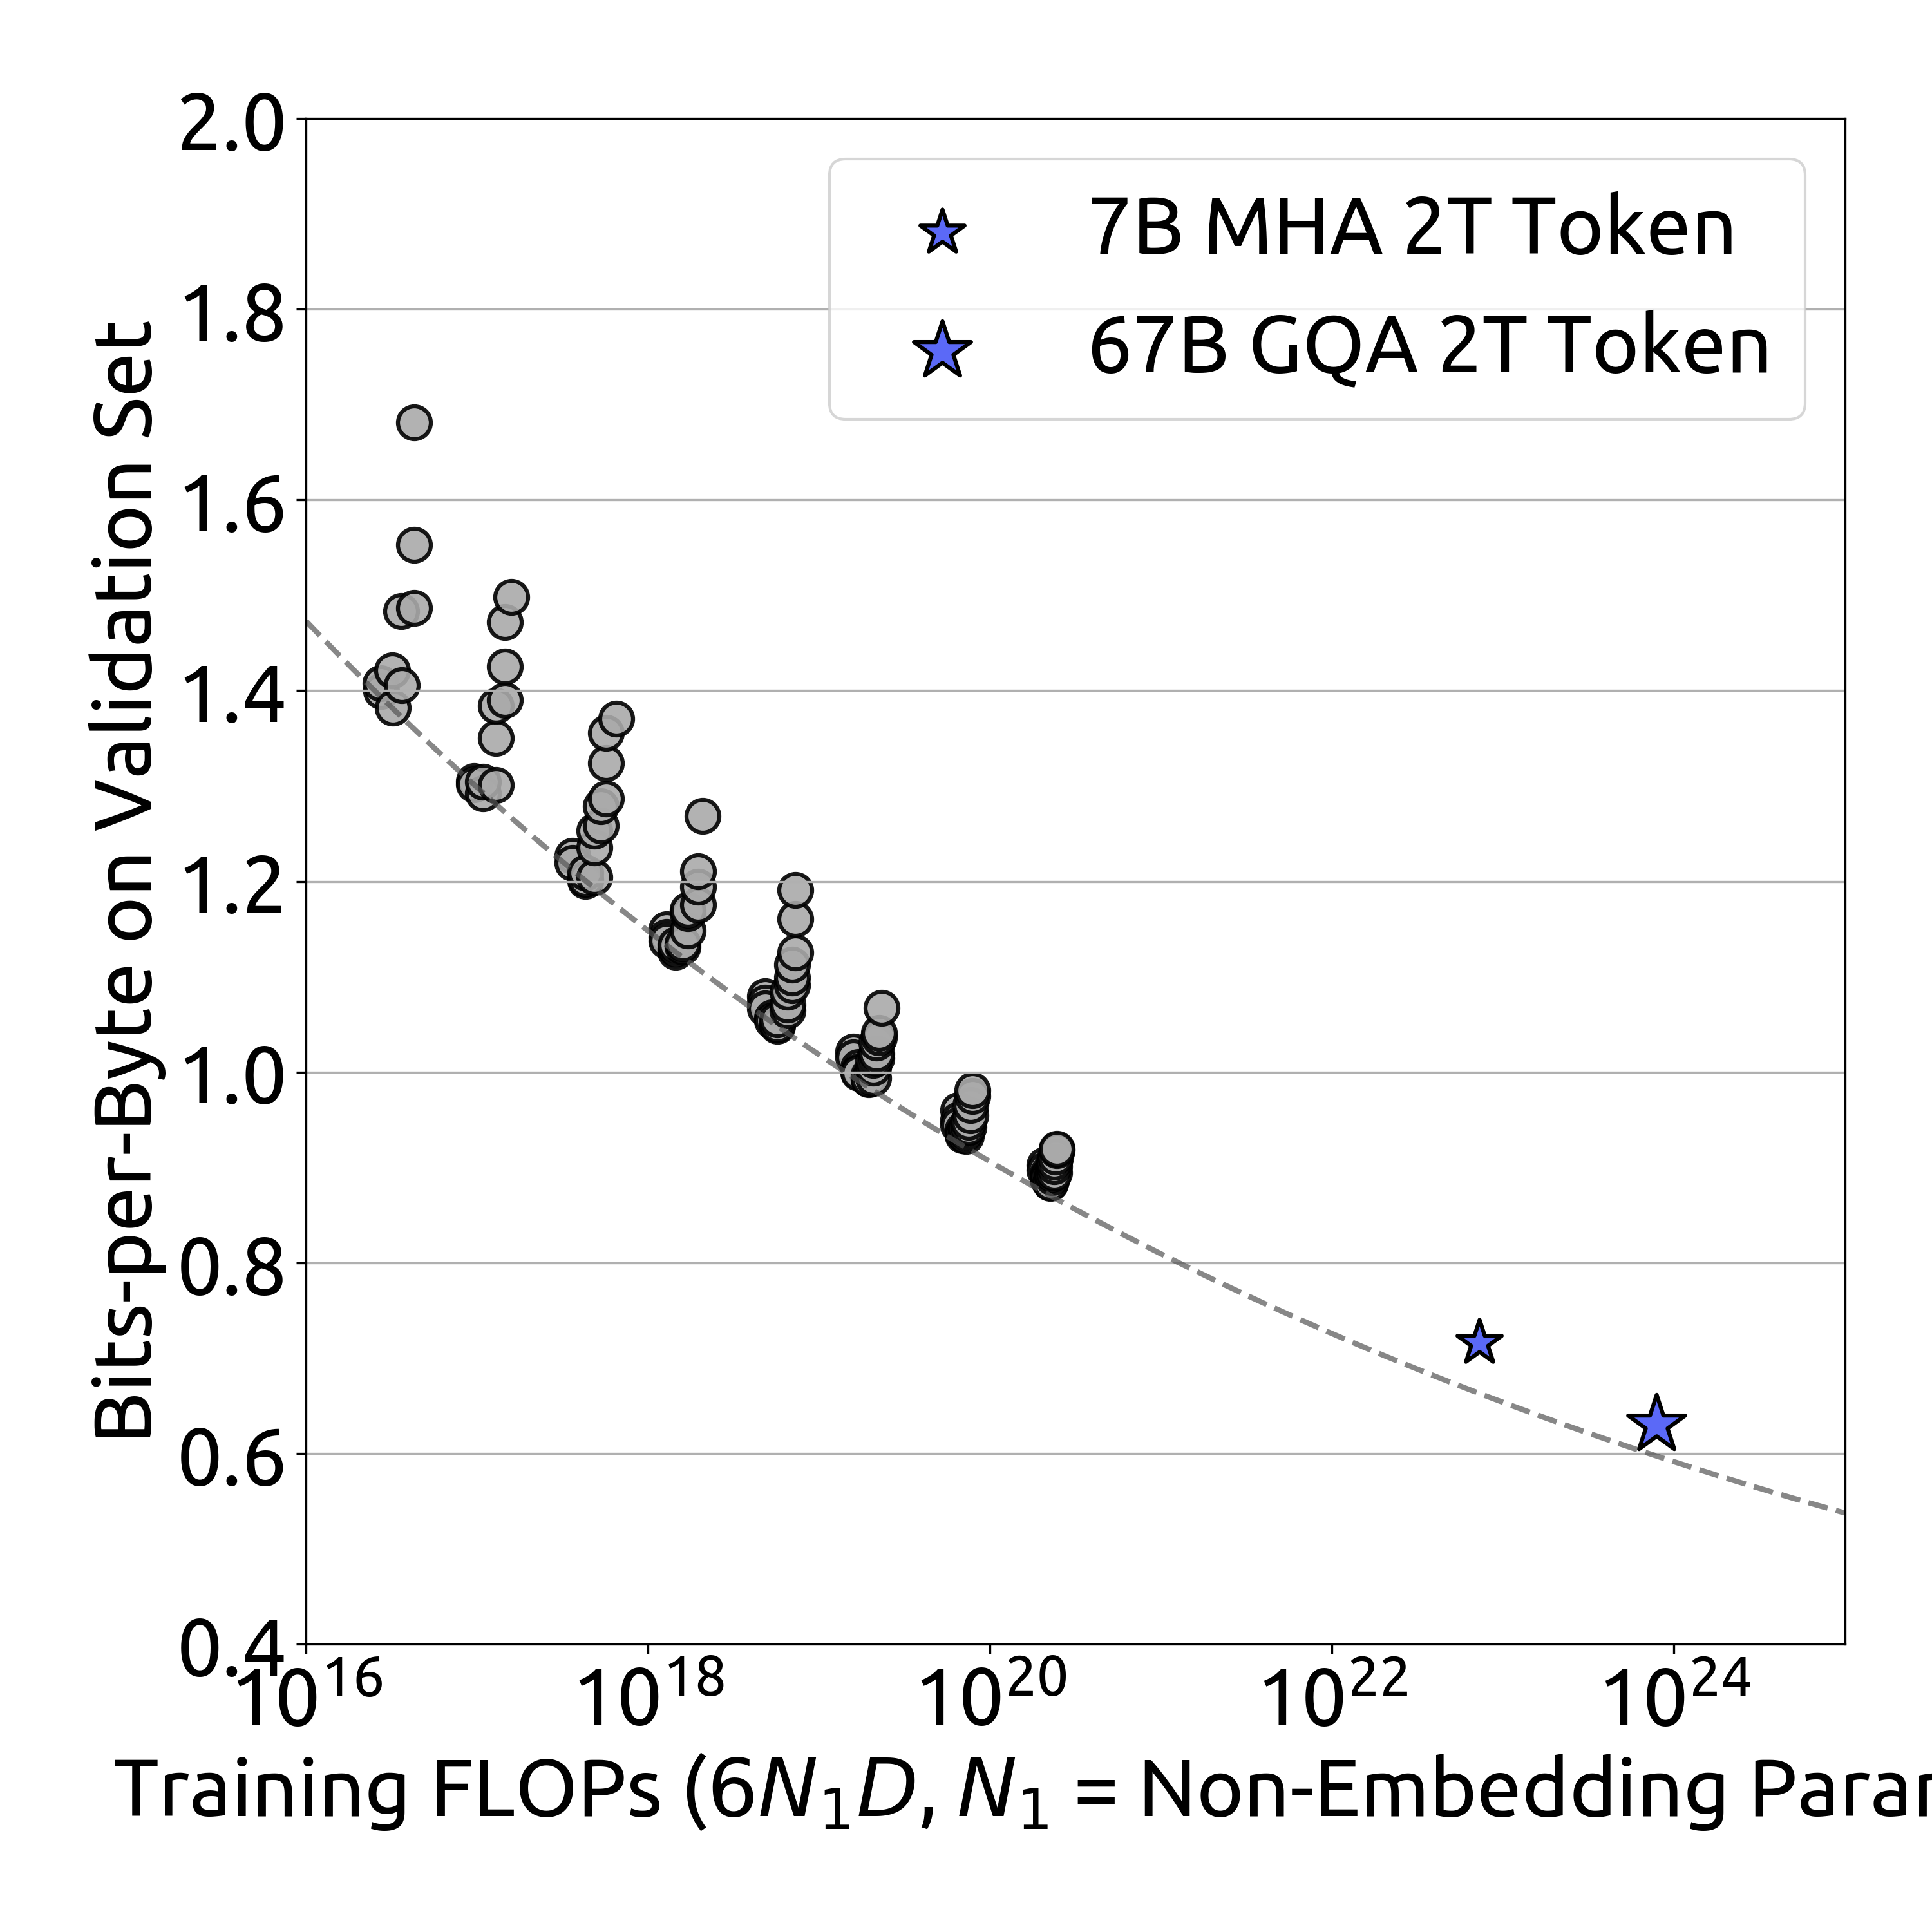
\includegraphics[width=0.31\textwidth]{figures/flops_bpb_6n1d.png}
        \label{fig:flops_bpb_6n1d}
    }
    \subfigure[Compute budget $C=6N_2D$]{
        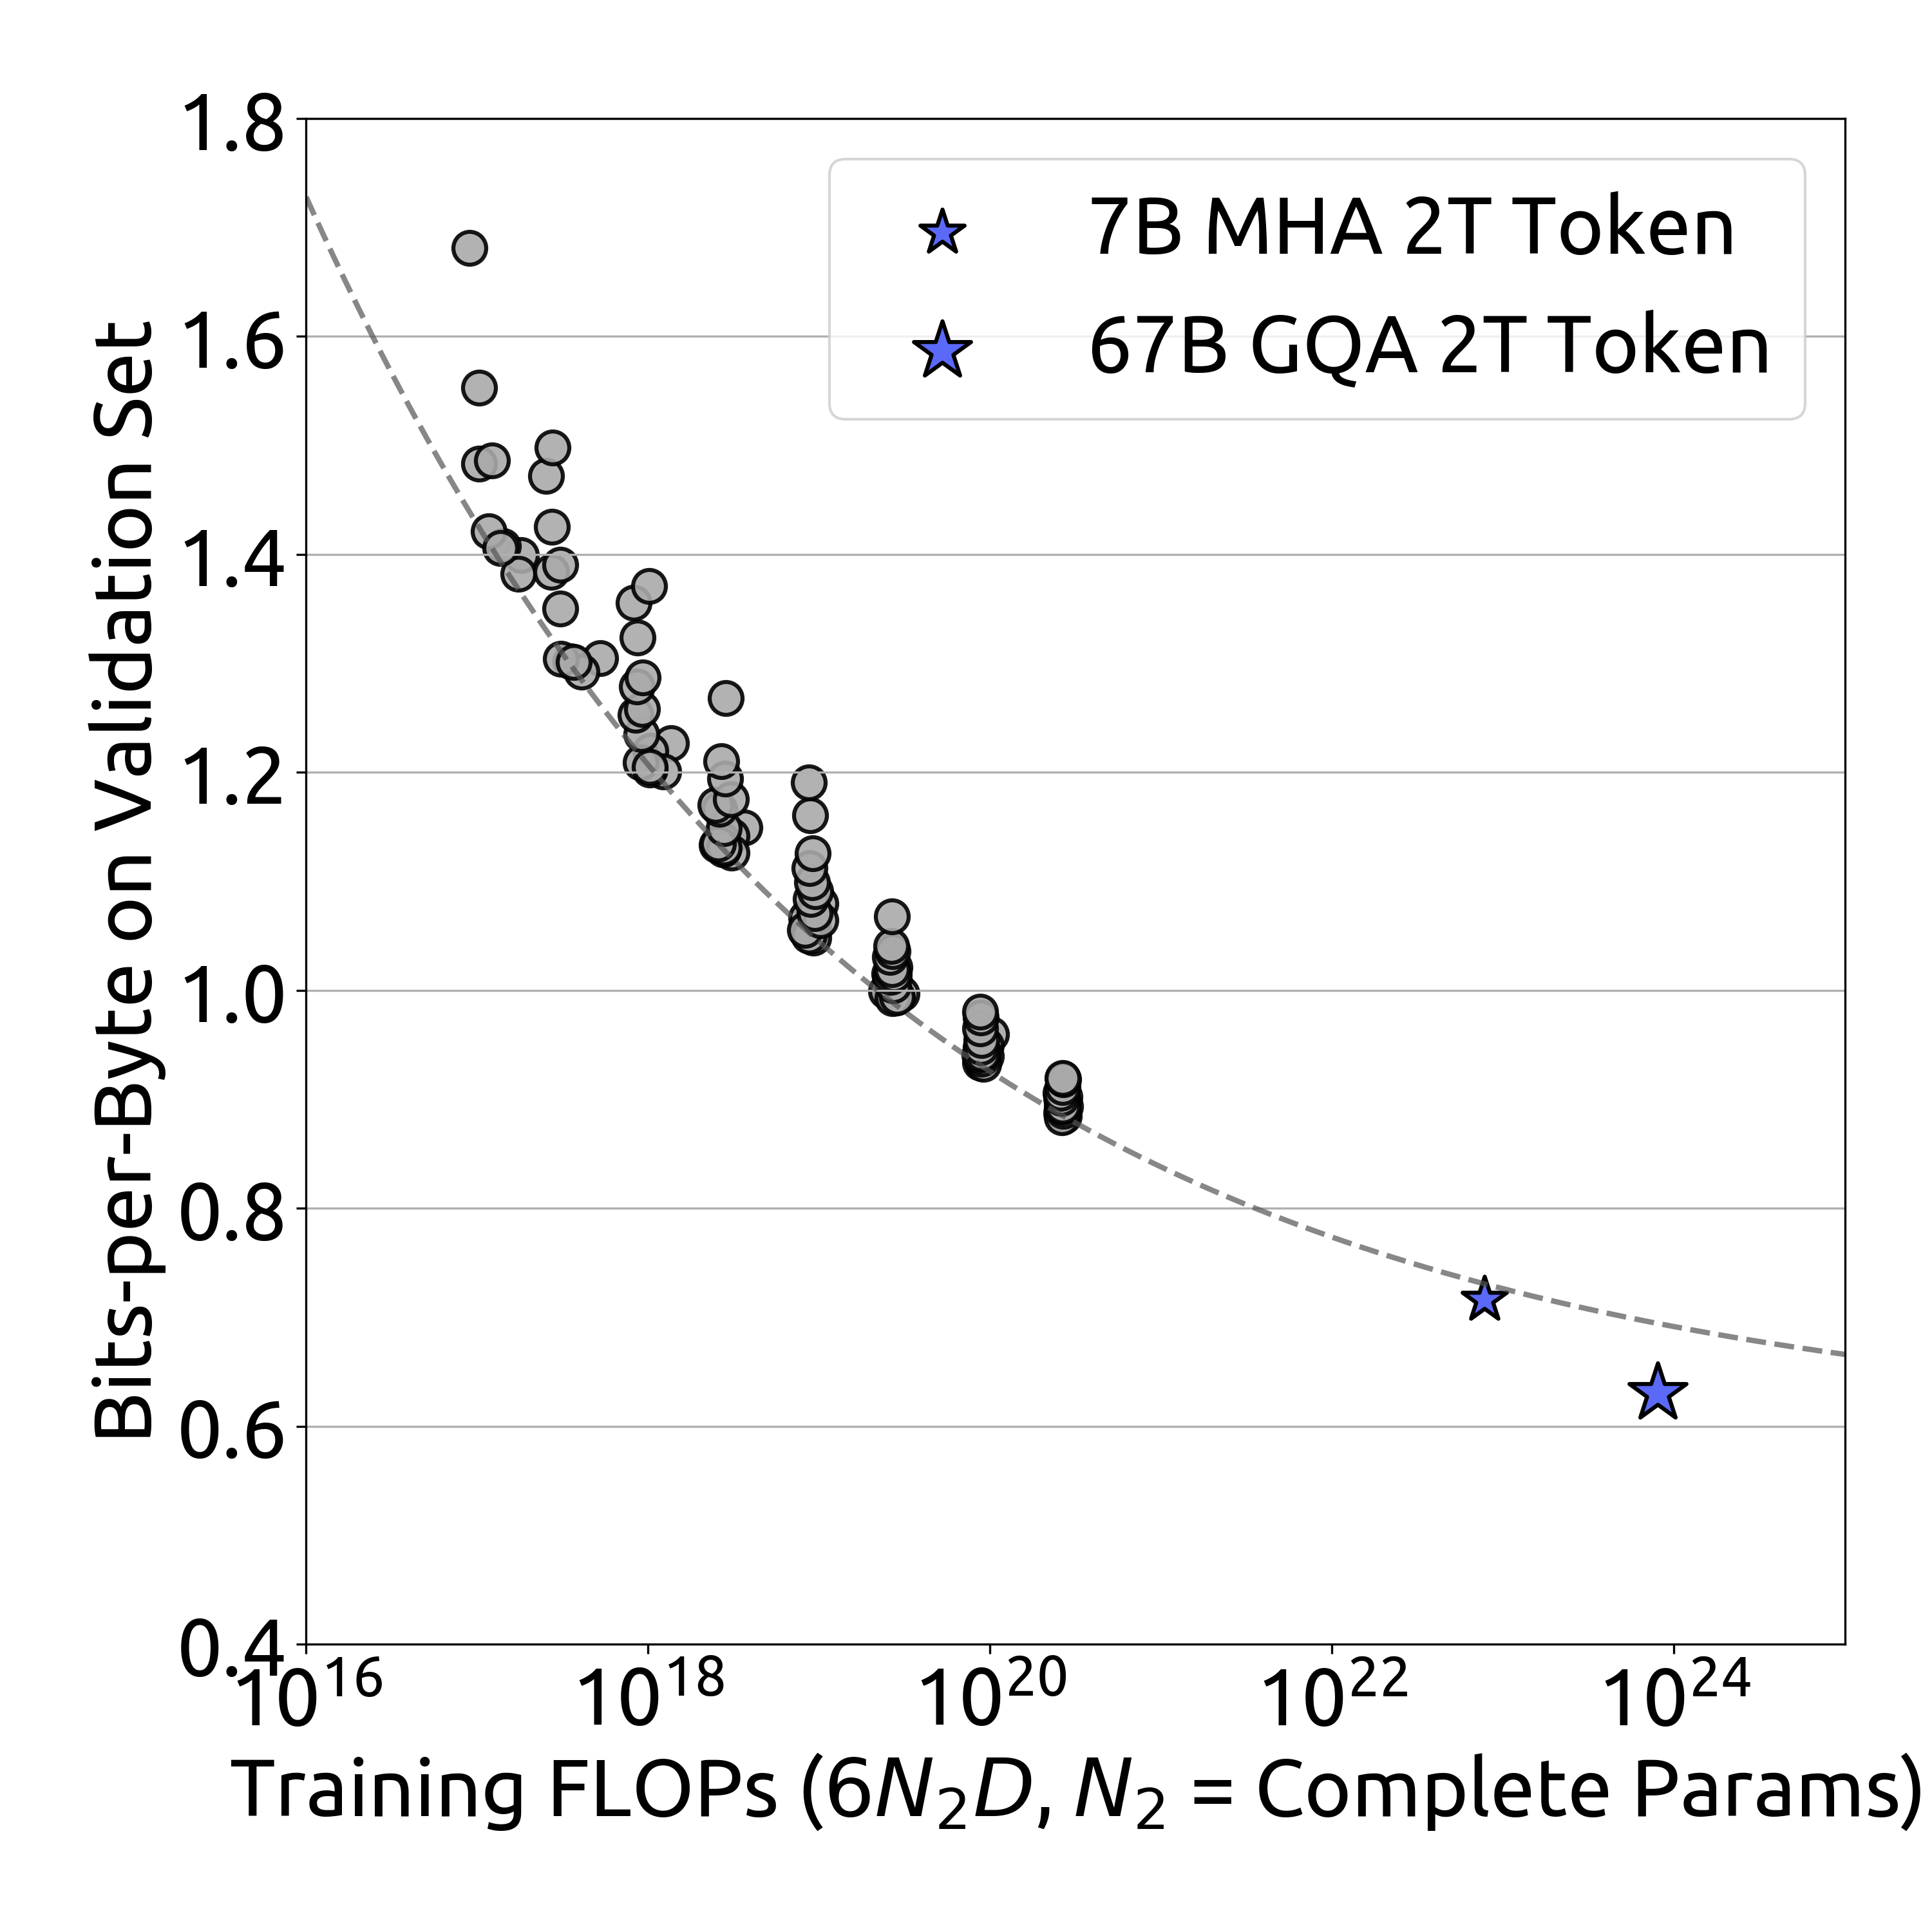
\includegraphics[width=0.31\textwidth]{figures/flops_bpb_6n2d.png}
        \label{fig:flops_bpb_6n2d}
    }
    \subfigure[Compute budget $C=MD$]{
        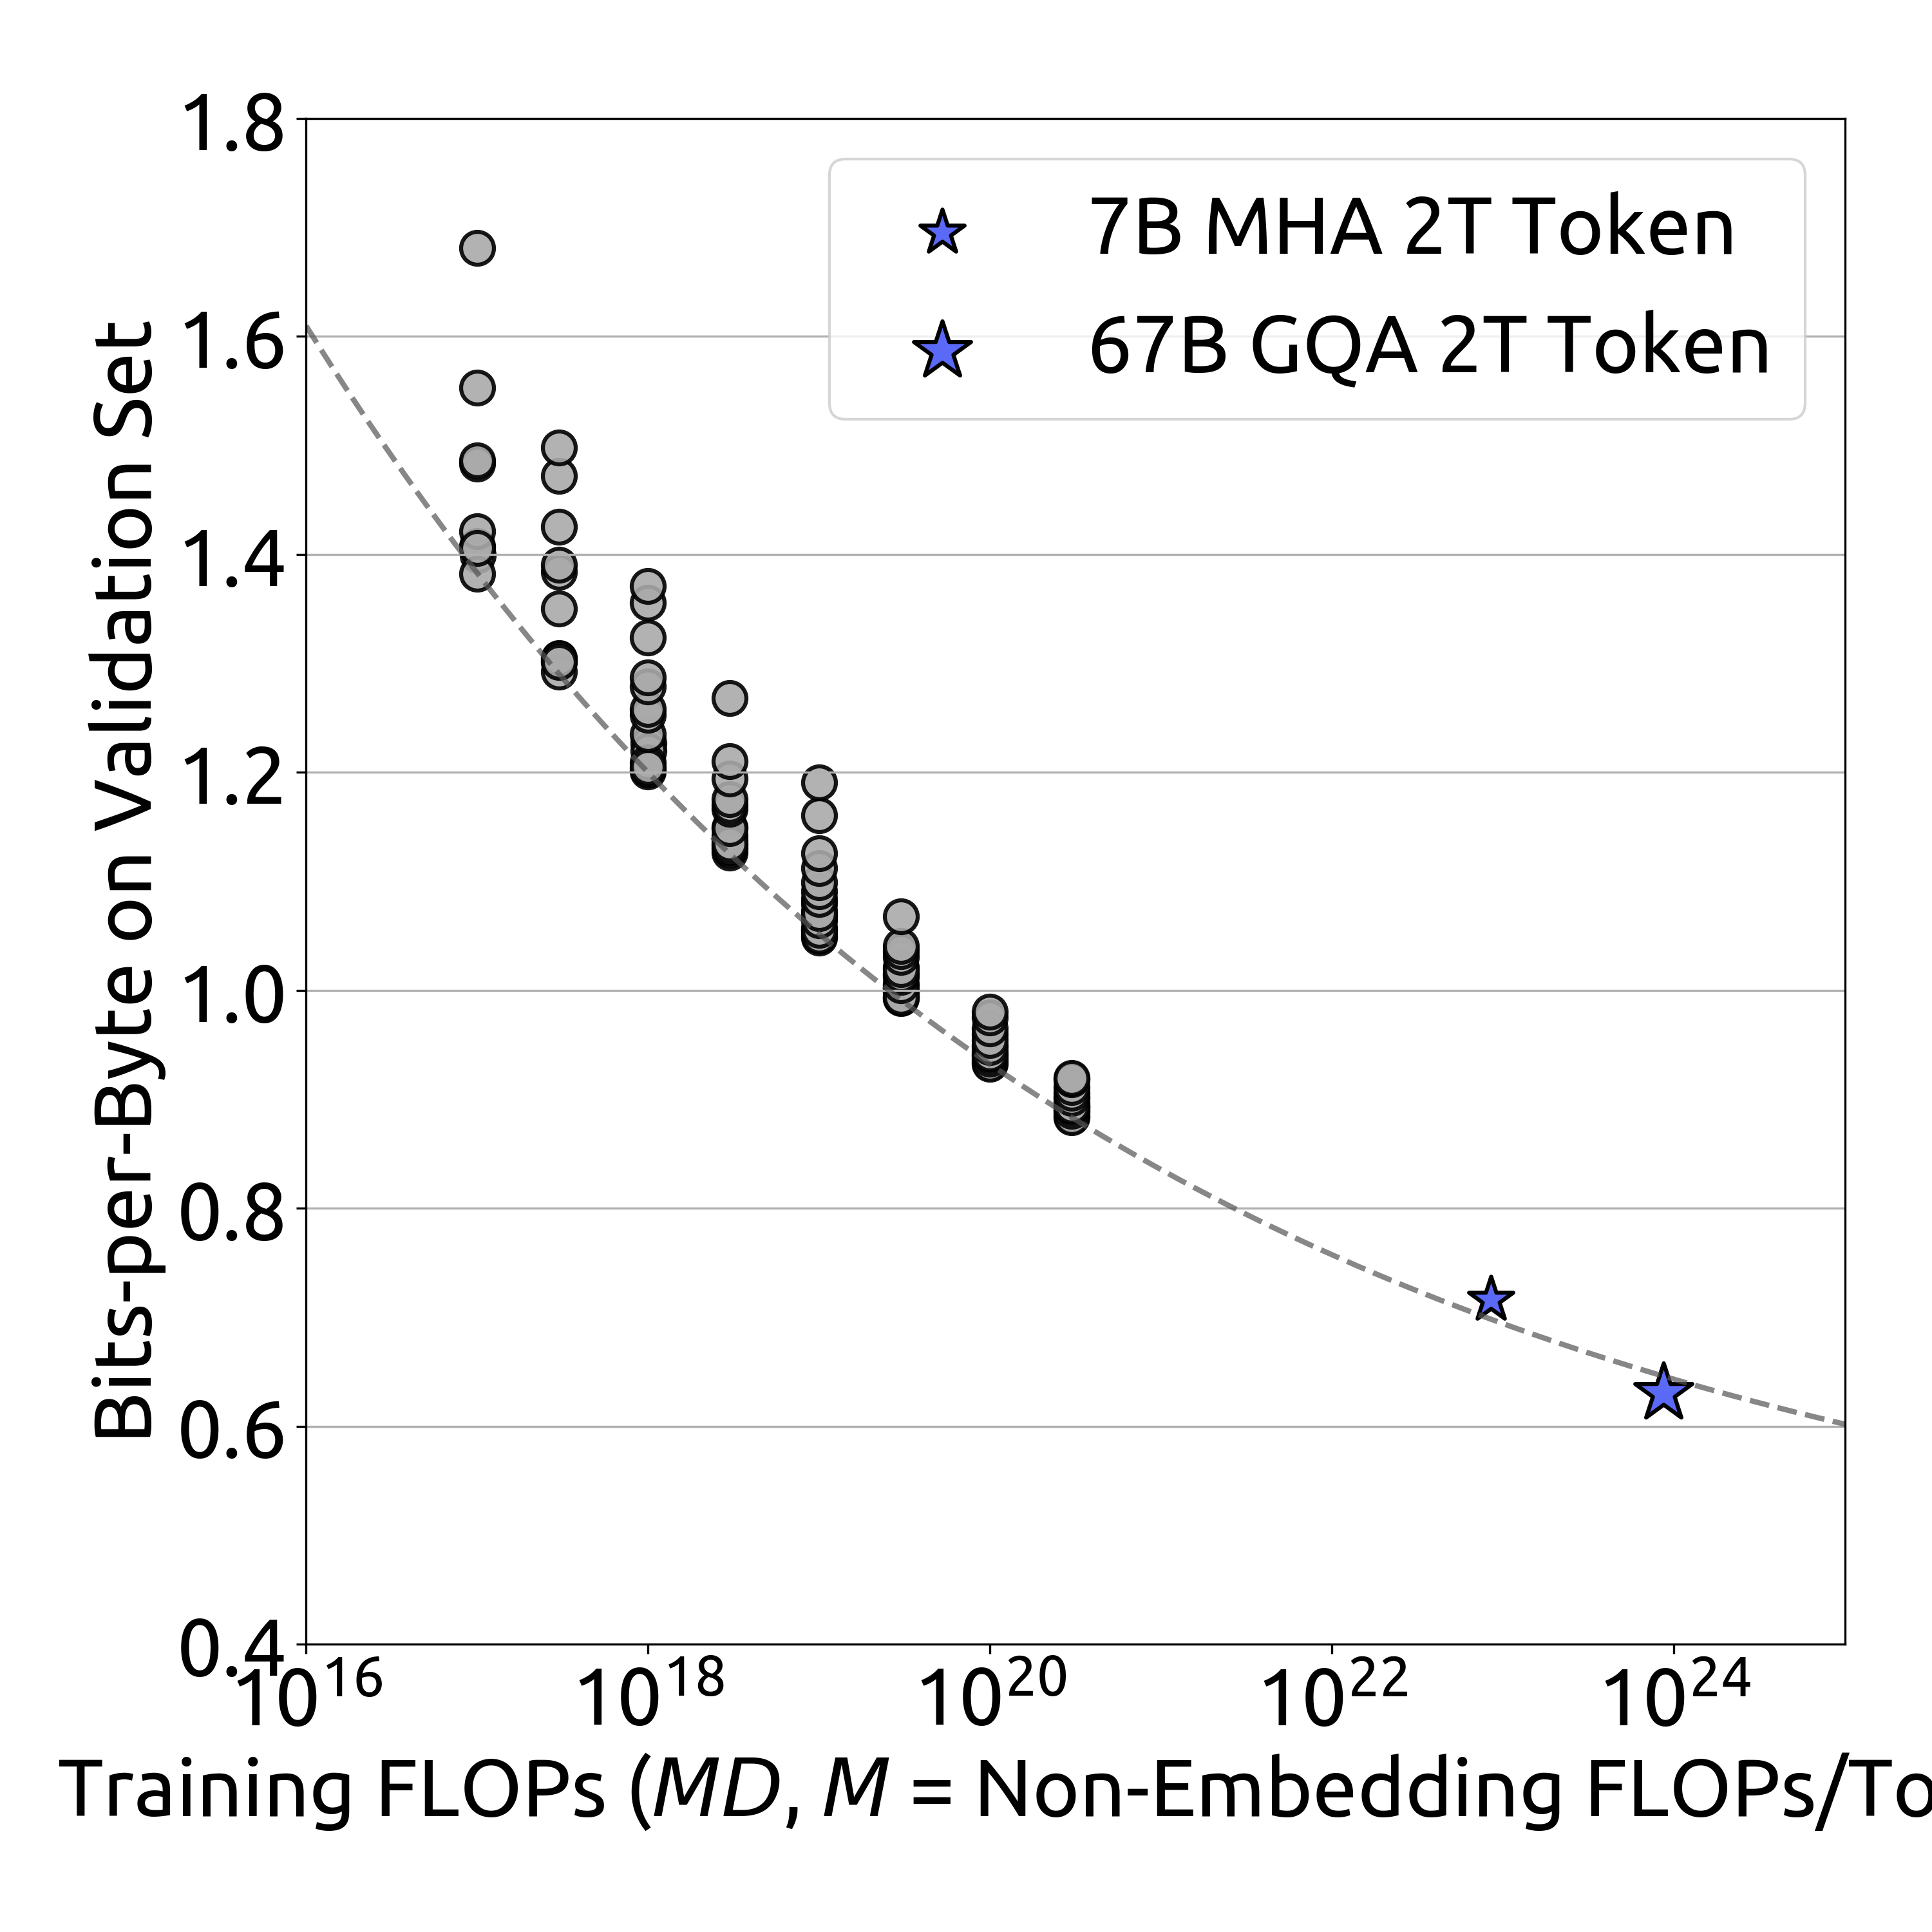
\includegraphics[width=0.31\textwidth]{figures/flops_bpb_md.png}
        \label{fig:flops_bpb_md}
    }
    \caption{Performance scaling curves using different model scale representations. The metric is the bits-per-byte on the validation set. The dotted line represents the power law fitting the smaller model (grey circles). The blue stars represent DeepSeek LLM 7B and 67B. $N_1$, $N_2$, and $M$ represent the non-embedding parameters, complete parameters, and non-embedding FLOPs/token of the model, respectively.}
    \label{fig:diff_model_scale}
\end{figure}

When using $6N_1$ as the model scale representation, the fitted performance scaling curve tends to overestimate the performance of large-scale models. Conversely, when using $6N_2$, the curve tends to underestimate their performance. Using $M$ as the model scale representation, however, achieves the most accurate predictions.



\subsection{Benchmark Metrics Curves}
\label{appendix:metric_curve}
\begin{figure}[h]
    \centering
    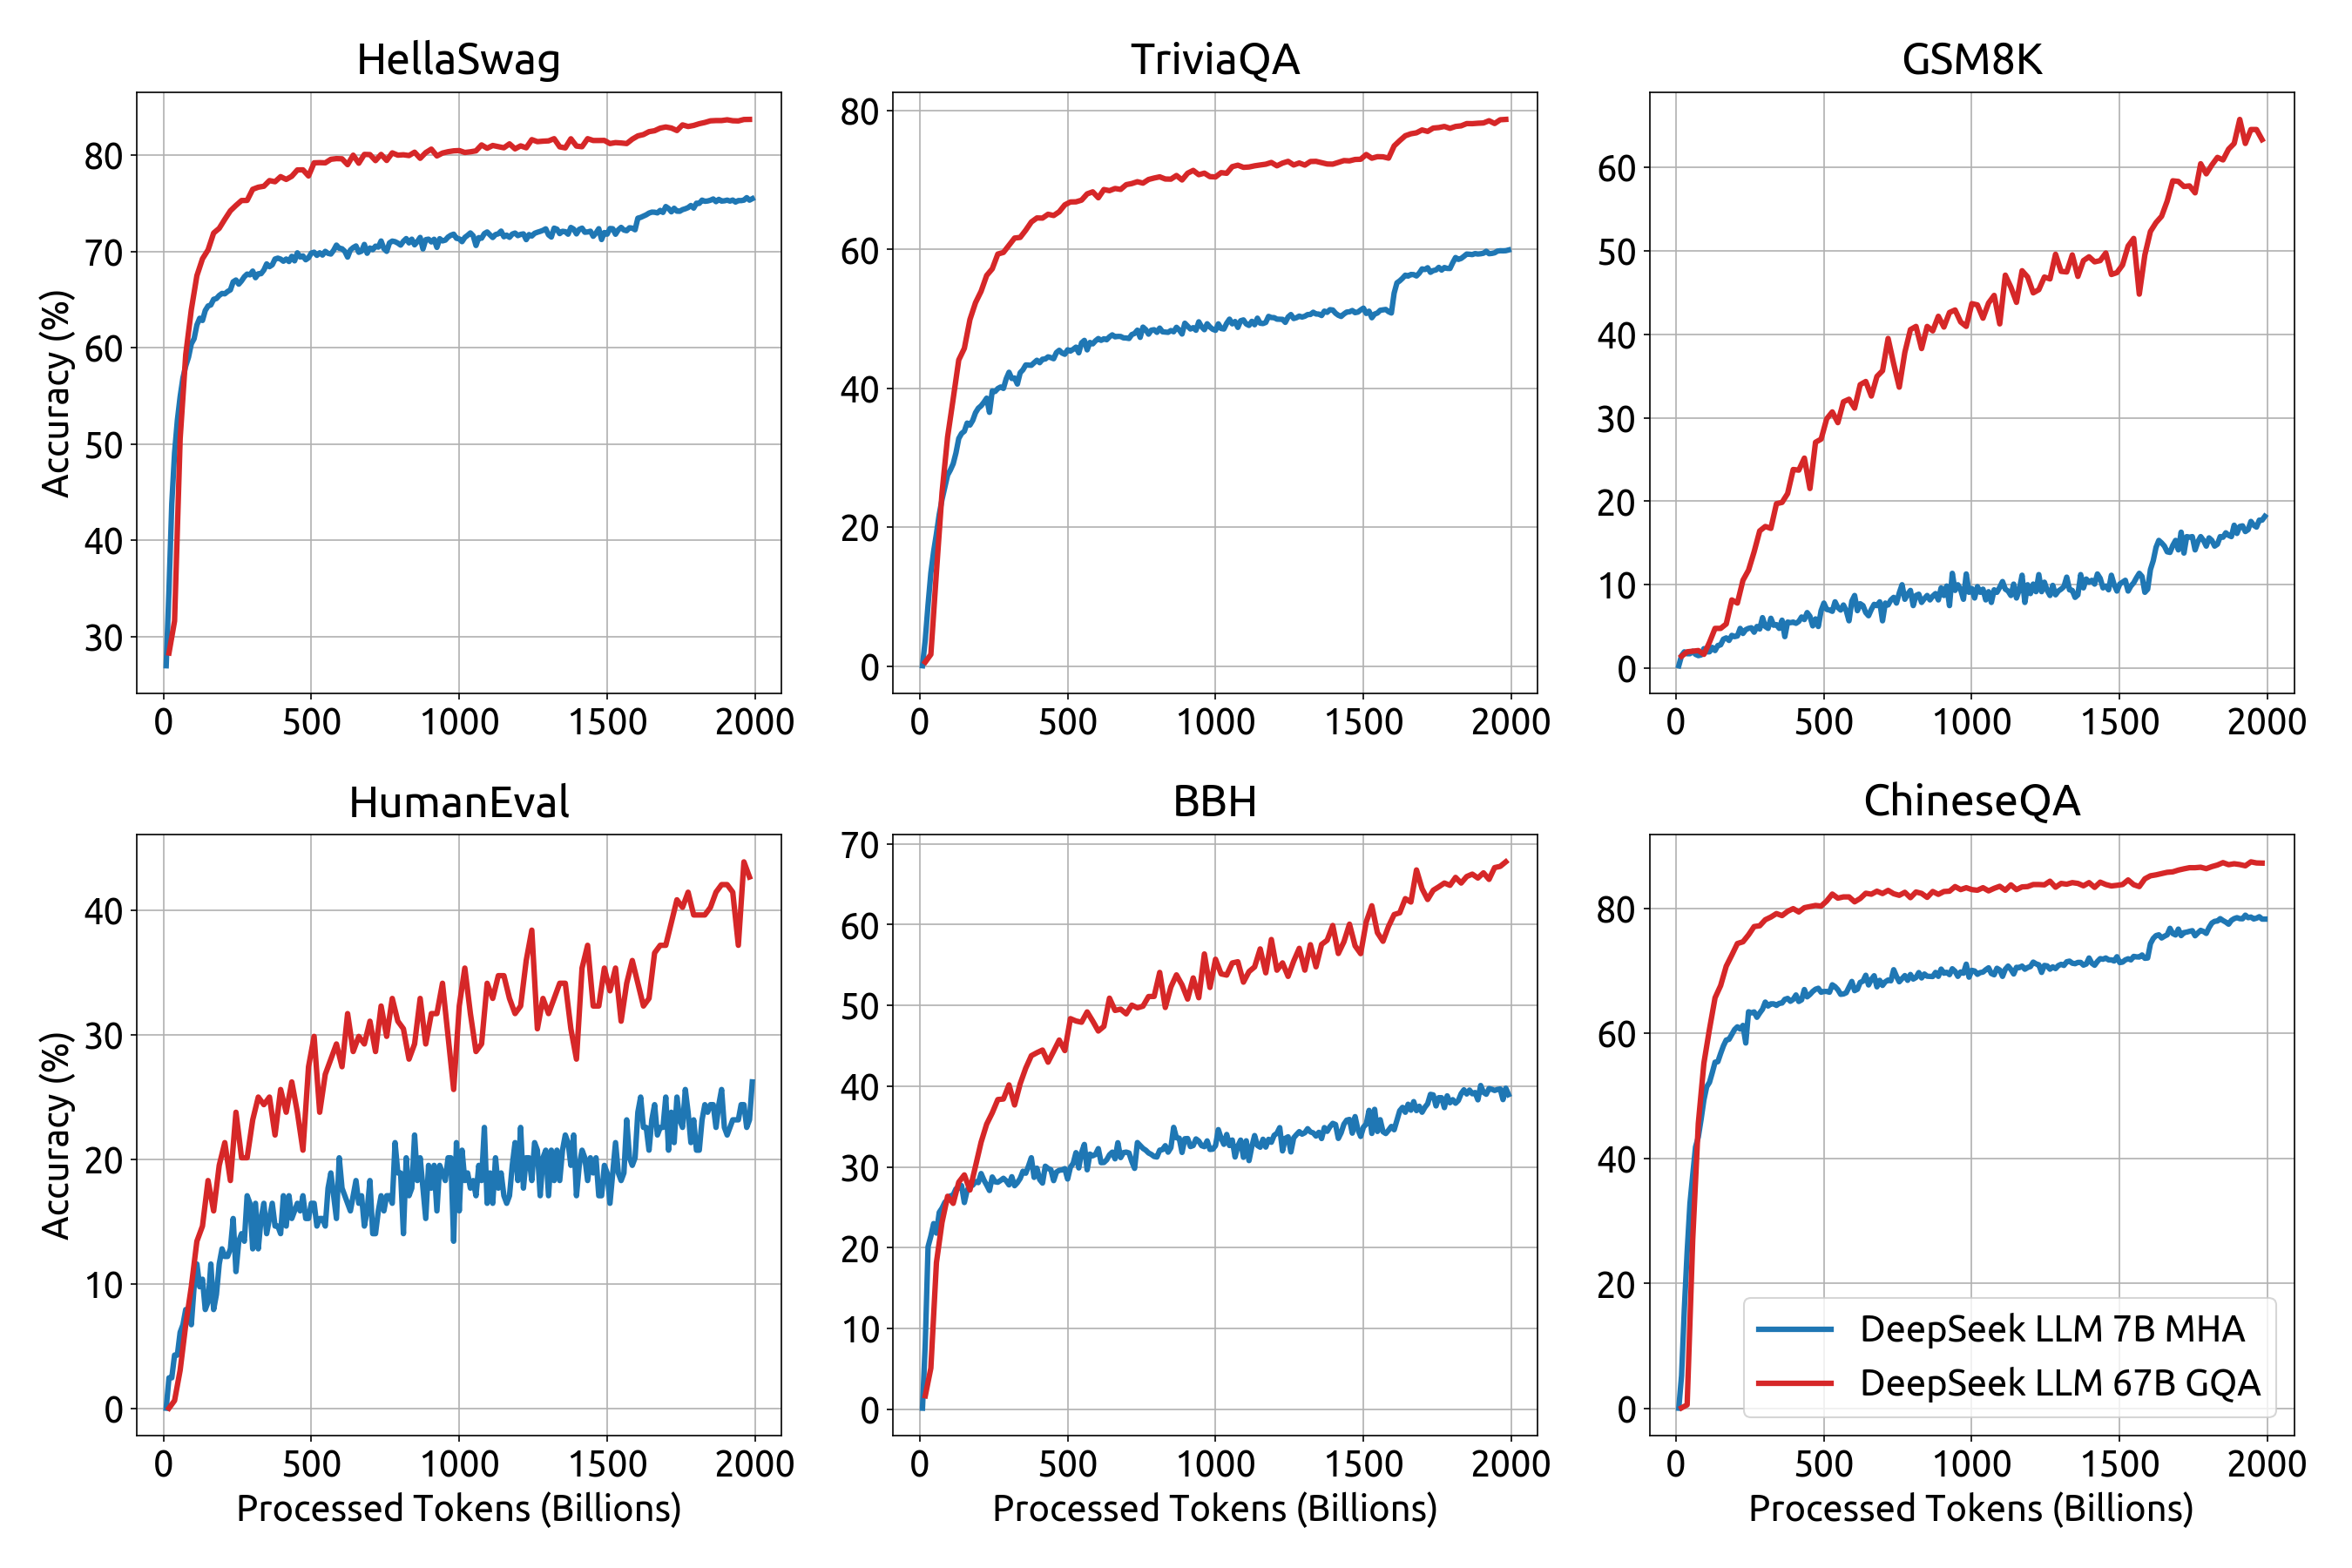
\includegraphics[width=0.8\textwidth]{figures/pretrain_metric.png}
    \caption{Benchmark metrics curves of DeepSeek LLM Base. ChineseQA is our in-house test set, constructed in a manner akin to TriviaQA.}
    \label{fig:bench_curve}
\end{figure}
Figure \ref{fig:bench_curve} shows benchmark metrics curves across different training steps. We can see consistent improvement on these benchmarks from the start to the end of training. We believe the performance will further be improved if the training continues. 

\begin{table}[h]
	%	\footnotesize
	
		\centering
        \small
        

            
		\begin{tabular}{lccccc}
			\toprule
                 \multirow{2}{*}{Model} & \multirow{2}{*}{Size} & \multicolumn{2}{c}{HumanEval} & \multirow{2}{*}{MBPP} \\
                 
                  & & Python & Multilingual & & \\
            \midrule
            \multicolumn{6}{c}{\bf{Pre-Trained Models}} \\
            \midrule
            Codex-001 & - & 33.5\% & 26.1\% & 45.9\%  \\
            StarCoder & 16B & 36.0\% & 28.7\% & 46.8\% \\
            CodeGeeX2 & 6B & 36.0\% & 24.5\% & 42.4\%  \\
            CodeLlama & 7B & 31.7\% & 29.2\% & 41.6\% \\
            CodeLlama & 13B & 36.0\% & 35.4\% & 48.4\%  \\
            CodeLlama & 34B & \textbf{48.2}\% & \textbf{41.0} \% & 55.2\% \\
           
            DeepSeek-LLM-Base & 67B & 42.7\% & 37.2\% & \textbf{57.4\%}  \\
            \midrule
            \multicolumn{6}{c}{\bf{Instruction-Tuned Models}} \\
            \midrule
            Wizard-Coder & 34B & 73.2\% & 48.8\% & 61.2\% \\
            DeepSeek-LLM-Chat & 67B & \textbf{73.8\%} & \textbf{53.3}\% & \textbf{61.4\%} &\\
		\bottomrule
		\end{tabular}
    
        	\caption{\centering Comparison with code-specific models. \label{table:compare-code}}
\end{table}

\subsection{Comparison with Code or Math Specific Models}
\label{sec:code-and-math}

We have conducted a comparison between our model and specific code and math language models (LLMs). Table \ref{table:compare-code} demonstrates that DeepSeek LLM 67B is capable of achieving similar performance to CodeLlama, despite having access to less code data. It is worth noting that DeepSeek LLM possesses greater capabilities in areas other than code. 

Likewise, Table \ref{table:math_results} presents the results obtained from various math-related benchmarks, such as GSM8K~\citep{gsm8k}, MATH~\citep{hendrycks2021measuring}, MGSM-zh~\citep{mgsm}, and CMath~\citep{wei2023cmath}. DeepSeek 67B exhibits exceptional performance on math-related tasks across different languages, showcasing its superiority in this domain. In addition, DeepSeek LLM can utilize programs to solve math problems, which demonstrates better performance than chain-of-thoughts. It is significantly better than the previous SOTA model, ToRA \citep{tora}, on the benchmarks. 

\begin{table}[h]
\centering
\small
\begin{tabular}{lccccc}
\toprule
&\textbf{Inference} & \textbf{GSM8K} & \textbf{MATH} & \textbf{MGSM-zh} & \textbf{CMath} \\
         \midrule
            \multicolumn{6}{c}{\bf{Chain-of-Thoughts}} \\
            \midrule
MetaMath 70B \citep{metamath} & CoT & 82.3\% & 26.6\% & 66.4\% & 70.9\% \\ 
WizardMath 70B \citep{wizardmath} & CoT  & 81.6\% & 22.7\% & 64.8\% & 65.4\% \\ 
DeepSeek LLM 67B Chat &CoT                & \textbf{84.1}\%         & \textbf{32.6} \%        & \textbf{74.0\%}           & \textbf{80.3\%}                    \\ 
            \midrule
            \multicolumn{6}{c}{\bf{Tool-Integrated Reasoning}} \\
            \midrule
ToRA-Code 34B \citep{tora} & Tool-Integrated & 80.7\% & 50.8\% & 41.2\% & 53.4\% \\ 
DeepSeek LLM 67B Chat  & Tool-Integrated & \textbf{86.7\%} & \textbf{51.1\%}        & \textbf{76.4\%}           & \textbf{85.4\%}                  \\ \bottomrule
\end{tabular}
\caption{\centering Comparison with math-specific models. \label{table:math_results}}

\end{table}



\subsection{Benchmark Results w/ DPO Stage}
Table \ref{tab: dpo} presents the benchmark results obtained with the DPO stage. Based on these results, we can conclude that the DPO stage does not significantly impact the fundamental capability of an LLM.
\begin{table}[h]
    \centering \small
\begin{tabular}{lcc}
\toprule
& DeepSeek 67B Chat & DeepSeek 67B Chat DPO \\ \midrule

HellaSwag & 75.7 & 76.1 \\

TriviaQA & 81.5 & 82.9 \\

NaturalQuestions & 47.0 & 48.8 \\

MMLU & 71.1 & 70.9 \\

GSM8K & 84.1 & 85.2 \\

MATH & 32.6 & 30.2 \\

HumanEval & 73.8 & 71.3 \\

BBH & 71.7 & 70.8 \\

AGIEval & 46.4 & 46.1 \\

CEval & 65.2 & 64.3 \\

CMMLU & 67.8 & 68.2 \\
\bottomrule
\end{tabular}
    \caption{\centering The benchmark metrics before and after DPO stage. }
    \label{tab: dpo}
\end{table}

\subsection{Evaluation Formats}
\label{appendix:eval_formats}
Table \ref{tab:agieval_eval_format_example}$\sim$Table \ref{tab:winogrande_eval_format_example} present examples of our evaluation formats on different benchmarks.
\input{tables/evaluation_formats}

\setcounter{figure}{0}
\makeatletter 
\renewcommand{\thefigure}{A\@arabic\c@figure}
\makeatother

\setcounter{table}{0}
\makeatletter 
\renewcommand{\thetable}{A\@arabic\c@table}
\makeatother

\end{CJK*}
\end{document} 